
\documentclass{article}
\usepackage[utf8]{inputenc}
\usepackage{mathtools}
\usepackage{amssymb}
\usepackage{amsmath}
\usepackage{listings}
\usepackage{braket}
\usepackage[toc,page]{appendix}

%%%THEOREM (ETC) ENVIRONMENTS
\newtheorem{definition}{Definition}
\newtheorem{claim}{Claim}
\newtheorem{conjecture}{Conjecture}
\newtheorem{corollary}{Corollary}
\newtheorem{example}{Example}
\newtheorem{problem}{Problem}
\newtheorem{idea}{Idea} 

\usepackage{proof}
\newtheorem{theorem}{Theorem}

\newtheorem{lemma}[theorem]{Lemma}
\newtheorem{proposition}[theorem]{Proposition}

\newenvironment{proof}[1][Proof]{\begin{trivlist}
\item[\hskip \labelsep {\bfseries #1}]}{\begin{flushright}$\blacksquare$\end{flushright} \end{trivlist}}
\newenvironment{remark}[1][Remark]{\begin{trivlist}
\item[\hskip \labelsep {\bfseries #1}]}{\end{trivlist}}

\newcommand{\cat}{\mathcal{C}}
\newcommand{\Tau}{\mathrm{T}}
\newcommand{\ham}{\mathcal{H}}
\title{Hopf Algebras in Quantum Computation}
\author{Giovanni de Felice}
\date{April 2017}

%%%TIKZ:
\usepackage{tikz,pgfplots}
\usetikzlibrary{shapes.geometric}
\usetikzlibrary{trees, patterns}
\usetikzlibrary{positioning}
\usepackage{tikz,ifthen,calc}
\usepackage{tkz-euclide}
\usetikzlibrary{shapes,snakes}
\usetikzlibrary{calc,intersections, fit, knots, hobby, positioning, patterns}
\usepackage{braids}

%%%categorical diagrams:
\tikzset{
	buffer/.style={
		draw,
		shape border rotate=180,
		regular polygon,
		regular polygon sides=3,
		node distance=2cm,
		minimum height=4em
	}
}
\tikzstyle{arr}=[markings,mark=at position 0.5 with {\arrow{<}}]
%%%HOPF ALGEBRAS:
\newcommand{\mult}{
	
\begin{tikzpicture}[scale=0.2, black/.style={scale=0.5,draw,shape=circle,fill=black}]
	\node[black] (0) at (0, 0) {};
	\draw (1,-1) to (0);
	\draw (-1,-1) to (0);
	\draw (0) to (0,1);
	\end{tikzpicture}
}
\newcommand{\unit}{
	
\begin{tikzpicture}[scale=0.2, black/.style={scale=0.5,draw,shape=circle,fill=black}]
	\node[black] (0) at (0, 0) {};
	\draw (0) to (0,1);
	\end{tikzpicture}
}
\newcommand{\comult}{
	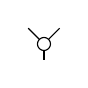
\begin{tikzpicture}[scale=0.2, black/.style={scale=0.5,draw,shape=circle,fill=white}]
	\node[black] (0) at (0, 0) {};
	\draw (1,1) to (0);
	\draw (-1,1) to (0);
	\draw (0) to (0,-1);
	\end{tikzpicture}
}

\newcommand{\counit}{
	\begin{tikzpicture}[scale=0.2, black/.style={scale=0.5,draw,shape=circle,fill=white}]
	\node[black] (0) at (0, 0) {};
	\draw (0) to (0,-1);
	\end{tikzpicture}
}

\newcommand{\antipode}{
	\begin{tikzpicture}[scale=0.2, black/.style={scale=0.5,draw,regular polygon,
		regular polygon sides=4,fill=white}]
	\node[scale=0.5, black] (0) at (0, 0) {$S$};
	\draw (0) to (0,-1);
	\draw (0) to (0,1);
	\end{tikzpicture}
}

\newcommand{\associativity}{
\begin{equation}
\begin{gathered}
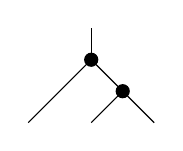
\begin{tikzpicture}[scale=0.8]
\node[scale=0.5,draw,circle,fill=black] (0) at (0,0.5) {};
\node[scale=0.5,draw,circle,fill=black] (1) at (0.5,0) {};
\draw (0) to (1);
\draw (-1,-0.5) to (0);
\draw (0,-0.5) to (1);
\draw (1,-0.5) to (1);
\draw (0) to (0,1);
\end{tikzpicture}
\end{gathered}
\, = \,
\begin{gathered}
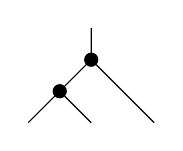
\begin{tikzpicture}[scale=0.8]
\node[scale=0.5,draw,circle,fill=black] (0) at (0.5,0.5) {};
\node[scale=0.5,draw,circle,fill=black] (1) at (0,0) {};
\draw (0) to (1);
\draw (-0.5,-0.5) to (1);
\draw (0.5,-0.5) to (1);
\draw (1.5,-0.5) to (0);
\draw (0) to (0.5,1);
\end{tikzpicture}
\end{gathered}
\end{equation}
}
\newcommand{\unitlaw}{
\begin{equation}
\begin{gathered}
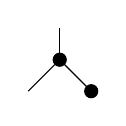
\begin{tikzpicture}[scale=0.8]
\node[scale=0.5,draw,circle,fill=black] (0) at (0,0.5) {};
\node[scale=0.5,draw,circle,fill=black] (1) at (0.5,0) {};
\draw (0) to (1);
\draw (-0.5,0) to (0);
\draw (0) to (0,1);
\end{tikzpicture}
\end{gathered}
\, = \,
\begin{gathered}
\begin{tikzpicture}[scale=0.8]
\draw (0,0) to (0,1);
\end{tikzpicture}
\end{gathered}
\, = \,
\begin{gathered}
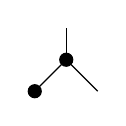
\begin{tikzpicture}[scale=0.8]
\node[scale=0.5,draw,circle,fill=black] (0) at (0,0.5) {};
\node[scale=0.5,draw,circle,fill=black] (1) at (-0.5,0) {};
\draw (0) to (1);
\draw (0.5,0) to (0);
\draw (0) to (0,1);
\end{tikzpicture}
\end{gathered}
\end{equation}
}
\newcommand{\coassociativity}{
\begin{equation}
\begin{gathered}
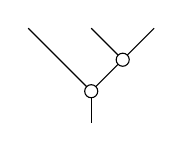
\begin{tikzpicture}[scale=0.8]
\node[scale=0.5,draw,circle,fill=white] (0) at (0,-0.5) {};
\node[scale=0.5,draw,circle,fill=white] (1) at (0.5,0) {};
\draw (0) to (1);
\draw (-1,0.5) to (0);
\draw (0,0.5) to (1);
\draw (1,0.5) to (1);
\draw (0) to (0,-1);
\end{tikzpicture}
\end{gathered}
\, = \,
\begin{gathered}
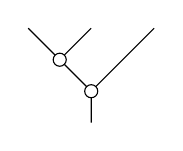
\begin{tikzpicture}[scale=0.8]
\node[scale=0.5,draw,circle,fill=white] (0) at (0.5,-0.5) {};
\node[scale=0.5,draw,circle,fill=white] (1) at (0,0) {};
\draw (0) to (1);
\draw (-0.5,0.5) to (1);
\draw (0.5,0.5) to (1);
\draw (1.5,0.5) to (0);
\draw (0) to (0.5,-1);
\end{tikzpicture}
\end{gathered}
\end{equation}
}
\newcommand{\counitlaw}{
\begin{equation}
\begin{gathered}
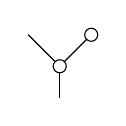
\begin{tikzpicture}[scale=0.8]
\node[scale=0.5,draw,circle,fill=white] (0) at (0,-0.5) {};
\node[scale=0.5,draw,circle,fill=white] (1) at (0.5,0) {};
\draw (0) to (1);
\draw (-0.5,0) to (0);
\draw (0) to (0,-1);
\end{tikzpicture}
\end{gathered}
\, = \,
\begin{gathered}
\begin{tikzpicture}[scale=0.8]
\draw (0,0) to (0,1);
\end{tikzpicture}
\end{gathered}
\, = \,
\begin{gathered}
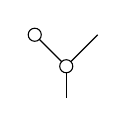
\begin{tikzpicture}[scale=0.8]
\node[scale=0.5,draw,circle,fill=white] (0) at (0,-0.5) {};
\node[scale=0.5,draw,circle,fill=white] (1) at (-0.5,0) {};
\draw (0) to (1);
\draw (0.5,0) to (0);
\draw (0) to (0,-1);
\end{tikzpicture}
\end{gathered}
\end{equation}
}

\newcommand{\bialgebralaw}{
\begin{equation}
\begin{gathered}
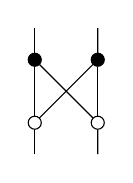
\begin{tikzpicture}[scale=0.8]
\node[scale=0.5,draw,circle,fill=white] (0) at (0,0) {};
\node[scale=0.5,draw,circle,fill=white] (1) at (1,0) {};
\node[scale=0.5,draw,circle,fill=black] (2) at (0,1) {};
\node[scale=0.5,draw,circle,fill=black] (3) at (1,1) {};
\draw (0) to (2);
\draw (0) to (3);
\draw (1) to (2);
\draw (1) to (3);
\draw (0,-0.5) to (0);
\draw (1,-0.5) to (1);
\draw (0,1.5) to (2);
\draw (1,1.5) to (3);
\end{tikzpicture}
\end{gathered}
\, = \,
\begin{gathered}
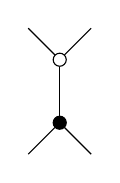
\begin{tikzpicture}[scale=0.8]
\node[scale=0.5,draw,circle,fill=black] (0) at (0.5,0) {};
\node[scale=0.5,draw,circle,fill=white] (1) at (0.5,1) {};
\draw (0) to (1);
\draw (0,-0.5) to (0);
\draw (1,-0.5) to (0);
\draw (0,1.5) to (1);
\draw (1,1.5) to (1);
\end{tikzpicture}
\end{gathered}
\end{equation}
}
\newcommand{\copylaw}{
\begin{equation}
\begin{gathered}
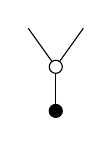
\begin{tikzpicture}[scale=0.7, squr/.style={scale=0.5,draw,regular polygon,
	regular polygon sides=4,fill=white}, black/.style={scale=0.5,draw,shape=circle,fill=black}, whit/.style={scale=0.5,draw,shape=circle,fill=white}]
\node[black] (0) at (0, 0) {};
\node[whit] (1) at  (0, 0.8) {};
\draw (0) to (1);
\draw (1) to (0.5,1.5);
\draw (1) to (-0.5,1.5);
\end{tikzpicture}
\end{gathered}
\, = \,
\begin{gathered}
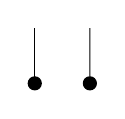
\begin{tikzpicture}[scale=0.7, black/.style={scale=0.5,draw,shape=circle,fill=black}]
\node[black] (0) at (0,0) {};
\node[black] (1) at (1,0) {};
\draw (0) to (0,1);
\draw (1) to (1,1);
\end{tikzpicture}
\end{gathered}
\end{equation}
}
\newcommand{\cocopylaw}{
	\begin{equation}
	\begin{gathered}
	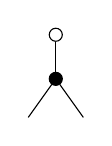
\begin{tikzpicture}[scale=0.7, squr/.style={scale=0.5,draw,regular polygon,
		regular polygon sides=4,fill=white}, black/.style={scale=0.5,draw,shape=circle,fill=black}, whit/.style={scale=0.5,draw,shape=circle,fill=white}]
	\node[whit] (0) at (0, 0) {};
	\node[black] (1) at  (0, -0.8) {};
	\draw (0) to (1);
	\draw (1) to (0.5,-1.5);
	\draw (1) to (-0.5,-1.5);
	\end{tikzpicture}
	\end{gathered}
	\, = \,
	\begin{gathered}
	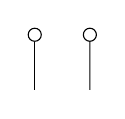
\begin{tikzpicture}[scale=0.7, black/.style={scale=0.5,draw,shape=circle,fill=white}]
	\node[black] (0) at (0,0) {};
	\node[black] (1) at (1,0) {};
	\draw (0) to (0,-1);
	\draw (1) to (1,-1);
	\end{tikzpicture}
	\end{gathered}
	\end{equation}
}
\newcommand{\hopflaw}{
	\begin{equation}
	\begin{gathered}
	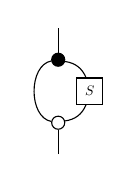
\begin{tikzpicture}[scale=0.8, squr/.style={scale=0.5,draw,regular polygon,
		regular polygon sides=4,fill=white}]
	\node[scale=0.5,draw,circle,fill=white] (0) at (0,0) {};
	\node[scale=0.5,draw,circle,fill=black] (1) at (0,1) {};
	\node[squr] (2) at (0.5,0.5) {$S$};
	\draw[bend left=80] (0) to (1);
	\draw[bend right] (0) to (2);
	\draw[bend right] (2) to (1);
	\draw (0,-0.5) to (0);
	\draw (0,1.5) to (1);
	\end{tikzpicture}
	\end{gathered}
	\, = \,
	\begin{gathered}
	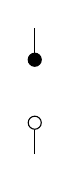
\begin{tikzpicture}[scale=0.8, squr/.style={draw,regular polygon,
		regular polygon sides=4,fill=white}]
	\node[scale=0.5,draw,circle,fill=white] (0) at (0,0) {};
	\node[scale=0.5,draw,circle,fill=black] (1) at (0,1) {};
	\draw (0,-0.5) to (0);
	\draw (0,1.5) to (1);
	\end{tikzpicture}
	\end{gathered}
	\, = \,
	\begin{gathered}
	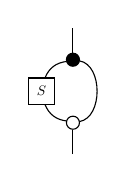
\begin{tikzpicture}[scale=0.8, squr/.style={scale=0.5,draw,regular polygon,
		regular polygon sides=4,fill=white}]
	\node[scale=0.5,draw,circle,fill=white] (0) at (0,0) {};
	\node[scale=0.5,draw,circle,fill=black] (1) at (0,1) {};
	\node[squr] (2) at (-0.5,0.5) {$S$};
	\draw[bend right=80] (0) to (1);
	\draw[bend left] (0) to (2);
	\draw[bend left] (2) to (1);
	\draw (0,-0.5) to (0);
	\draw (0,1.5) to (1);
	\end{tikzpicture}
	\end{gathered}
	\end{equation}
}
\newcommand{\modulelaw}{
	\begin{equation}
	\begin{gathered}
	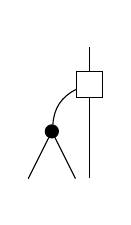
\begin{tikzpicture}[scale=0.6, squr/.style={draw,regular polygon,
		regular polygon sides=4,fill=white}, black/.style={scale=0.5,draw,shape=circle,fill=black}]
	\node (0) at (0, -2.2) {};
	\node[squr] (1) at (0, 0) {};
	\node (2) at (0, 1) {};
	\node[black] (3) at (-0.8, -1) {};
	\draw (0) to (1);
	\draw (1) to (2);
	\draw[bend left] (3) to (1);
	\draw (-1.3, -2) to (3);
	\draw (-0.3, -2) to (3);
	\end{tikzpicture}
	\end{gathered}
	\, = \,
	\begin{gathered}
	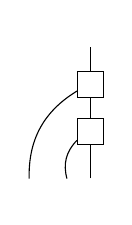
\begin{tikzpicture}[scale=0.6, squr/.style={draw,regular polygon,
		regular polygon sides=4,fill=white}, black/.style={draw,shape=circle,fill=black}]
	\node (0) at (0, -2.2) {};
	\node[squr] (1) at (0, 0) {};
	\node (2) at (0, 1) {};
	\node[squr] (3) at (0, -1) {};
	\draw (0) to (3);
	\draw (3) to (1);
	\draw (1) to (2);
	\draw (3) to (1);
	\draw[bend left] (-1.3, -2) to (1);
	\draw[bend left] (-0.5, -2) to (3);
	\end{tikzpicture}
	\end{gathered}
	\end{equation}
}
\newcommand{\comodulelaw}{
	\begin{equation}
	\begin{gathered}
	\begin{tikzpicture}[scale=0.6, squr/.style={draw,regular polygon,
		regular polygon sides=4,fill=white}, black/.style={scale=0.5,draw,shape=circle,fill=white}]
	\node (0) at (0, 2.2) {};
	\node[squr] (1) at (0, 0) {};
	\node (2) at (0, -2) {};
	\node[black] (3) at (-0.8, 1) {};
	\draw (0) to (1);
	\draw (1) to (2);
	\draw[bend right] (3) to (1);
	\draw (-1.3, 2) to (3);
	\draw (-0.3, 2) to (3);
	\end{tikzpicture}
	\end{gathered}
	\, = \,
	\begin{gathered}
	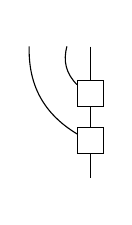
\begin{tikzpicture}[scale=0.6, squr/.style={draw,regular polygon,
		regular polygon sides=4,fill=white}, black/.style={draw,shape=circle,fill=black}]
	\node (0) at (0, 2.2) {};
	\node[squr] (1) at (0, 0) {};
	\node (2) at (0, -1) {};
	\node[squr] (3) at (0, 1) {};
	\draw (0) to (3);
	\draw (3) to (1);
	\draw (1) to (2);
	\draw (3) to (1);
	\draw[bend right] (-1.3, 2) to (1);
	\draw[bend right] (-0.5, 2) to (3);
	\end{tikzpicture}
	\end{gathered}
	\end{equation}
}
\newcommand{\intertwinerlaw}{
\begin{equation}
\begin{gathered}
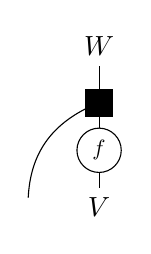
\begin{tikzpicture}[scale=0.6, squr/.style={draw,regular polygon,
	regular polygon sides=4,fill=black}]
\node (0) at (0, -2.2) {$V$};
\node[squr] (1) at (0, 0) {};
\node (2) at (0, 1.2) {$W$};
\node[scale=0.8,draw,circle] (3) at (0, -1) {$f$};
\draw (0) to (3);
\draw (3) to (1);
\draw (1) to (2);
\draw (3) to (1);
\draw[bend left] (-1.5, -2) to (1);
\end{tikzpicture}	
\end{gathered}
\, = \,
\begin{gathered}
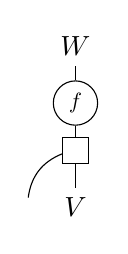
\begin{tikzpicture}[scale=0.6, squr/.style={draw,regular polygon,
	regular polygon sides=4,fill=white}]
\node (0) at (0, -2.2) {$V$};
\node[scale=0.8,draw,circle] (1) at (0, 0) {$f$};
\node (2) at (0, 1.2) {$W$};
\node[squr] (3) at (0, -1) {};
\draw (0) to (3);
\draw (3) to (1);
\draw (1) to (2);
\draw (3) to (1);
\draw[bend left] (-1, -2) to (3);
\end{tikzpicture}	
\end{gathered}
\end{equation}
}
\newcommand{\symAB}{
	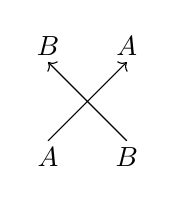
\begin{tikzpicture}[decoration={markings,mark=at position 0.5 with {\arrow{>}}}]
	\node (0) at (-0.5, -0.7) {$A$};
	\node (0) at (-0.5, 0.7) {$B$};
	\node (1) at (0.5, -0.7) {$B$};
	\node (1) at (0.5, 0.7) {$A$};
	\draw [->] (-0.5, -0.5) to (0.5, 0.5);
	\draw [->] (0.5, -0.5) to (-0.5, 0.5);
	\end{tikzpicture}
}

\newcommand{\symequation}{
	\begin{equation*}
	\begin{gathered}
	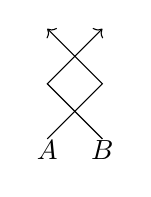
\begin{tikzpicture}[scale=0.7]
	\node (0) at (-1, -1.2) {$A$};
	\node (0) at (0, -1.2) {$B$};
	\draw [->] (-1, -1)--(0,0)--(-1,1);
	\draw [->] (0, -1)--(-1,0)--(0,1);
	\end{tikzpicture}
	\end{gathered}
	\, = \,
	\begin{gathered}
	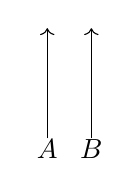
\begin{tikzpicture}[scale=0.7]
	\node (0) at (-0.8, -1.2) {$A$};
	\node (0) at (0, -1.2) {$B$};
	\draw [->] (-0.8, -1)--(-0.8,1);
	\draw [->] (0, -1)--(0,1);
	\end{tikzpicture}
	\end{gathered}
	\end{equation*}
}

\newcommand{\cupA}{	
	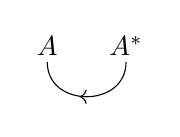
\begin{tikzpicture}[decoration={markings,mark=at position 0.5 with {\arrow{<}}}]
	\node (0) at (0, 0.2) {$A$};
	\node (1) at (1, 0.2) {$A^*$};
	\draw [bend right=90, looseness=1.5, postaction=decorate] (0,0) to (1,0);
	\end{tikzpicture}}

\newcommand{\capA}{	
	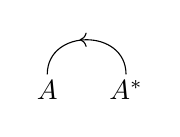
\begin{tikzpicture}[decoration={markings,mark=at position 0.5 with {\arrow{<}}}]
	\node (0) at (0, -0.2) {$A$};
	\node (1) at (1, -0.2) {$A^*$};
	\draw [bend left=90, looseness=1.5, postaction=decorate] (0,0) to (1,0);
	\end{tikzpicture}}

\newcommand{\snake}{
	\begin{equation*}
	\begin{gathered}
	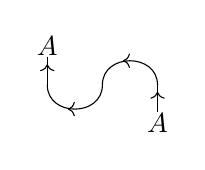
\begin{tikzpicture}[scale=0.7,decoration={markings,mark=at position 0.5 with {\arrow{<}}}]
	\node (0) at (0, 0.7) {$A$};
	\node (4) at (2, -0.7){$A$};
	\draw [bend right=90, looseness=1.5, postaction=decorate] (0, 0) to (1, 0);
	\draw [bend left=90, looseness=1.5, postaction=decorate] (1, 0) to (2, 0);
	\draw [postaction=decorate] (2, 0) to (2, -0.5);
	\draw [postaction=decorate] (0, 0.5) to (0, 0);
	\end{tikzpicture}
	\end{gathered}
	\, = \,
	\begin{gathered}
	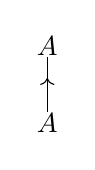
\begin{tikzpicture}[scale=0.7,decoration={markings,mark=at position 0.5 with {\arrow{<}}}]
	\node (0) at (0, 0.7) {$A$};
	\node (4) at (0, -0.7){$A$};
	\draw [postaction=decorate] (0, 0.5) to (0, -0.5);
	\end{tikzpicture}
	\end{gathered}
	\end{equation*}}

\newcommand{\snakestar}{
	\begin{equation*}
	\begin{gathered}
	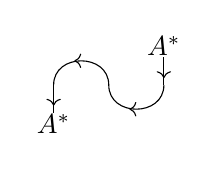
\begin{tikzpicture}[scale=0.7,decoration={markings,mark=at position 0.5 with {\arrow{<}}}]
	\node (0) at (0, -0.7) {$A^*$};
	\node (4) at (2, 0.7){$A^*$};
	\draw [bend left=90, looseness=1.5, postaction=decorate] (0, 0) to (1, 0);
	\draw [bend right=90, looseness=1.5, postaction=decorate] (1, 0) to (2, 0);
	\draw [postaction=decorate] (2, 0) to (2, 0.5);
	\draw [postaction=decorate] (0, -0.5) to (0, 0);
	\end{tikzpicture}
	\end{gathered}
	\, = \,
	\begin{gathered}
	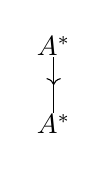
\begin{tikzpicture}[scale=0.7,decoration={markings,mark=at position 0.5 with {\arrow{>}}}]
	\node (0) at (0, 0.7) {$A^*$};
	\node (4) at (0, -0.7){$A^*$};
	\draw [postaction=decorate] (0, 0.5) to (0, -0.5);
	\end{tikzpicture}
	\end{gathered}
	\end{equation*}
}

\newcommand{\fusionijk}{
	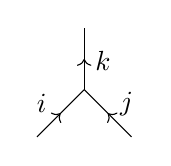
\begin{tikzpicture}[scale=0.6,decoration={markings,mark=at position 0.5 with {\arrow{>}}}]
	\node (0) at (-0.9, -0.3) {$i$};
	\node (1) at (0.9, -0.3) {$j$};
	\node (2) at (0.4, 0.6) {$k$};
	\draw [postaction=decorate] (-1, -1) to(0,0);
	\draw [postaction=decorate] (1,-1) to (0,0);
	\draw [postaction=decorate] (0,0) to (0,1.3);
	\end{tikzpicture}}
%%%%%%%%%%%%%%%%%%%%%%%%%%%%%%%%%%%%%%%%%%%%%%%%%%%%%%%%%%%%%%%%%%%%%%%%%%%%%%%%%%%%%%%%%%%%%%%%%%%%%%%%%%%%%%%%%%%%%%%%%%%%%%%%%%%%%%%%%%%%%%%%%%%%%%%%%%%%%%%%%%%%%%%%%%%%%%%%%%%%


\begin{document}
\maketitle
\tableofcontents

\pagebreak
\section{Introduction}
Categories and diagrams \\
Symmetry, quantization and categorification \\
Categorification = replacing equalities with isomorphisms \cite{Baez98}.\\
For an account of the relationships between categorification and quantization consider \cite{Rowell17}.\\
Mathematically: from groups to quasitriangular hopf algebras, G to DG\\
Categorically: from symmetric fusion categories to modular categories\\
Physically: fermions/bosons to anyons, local symmetries to topological symmetries, 3D to 2D\\
Computation: from PQC to TQC, complexity theory\\
Logic: mirror the relationship, all statements about RepDG are statements in RepG, a modality, programming language
%%%%%%%%%%%%%%%%%%%%%%%%%%%%%%%%%%%%%%%%%%%%%%%%%%%%%%%%%%%%%%%%%%%%%%%%%%%%%%%%%%%%%%%%%%%%%%%%%%%%%%%%%%%%%%%%%%%%%%%%%%%%%%%%%%%%%%%%%%%%%%%%
%%%%%%%%%%%%%%%%%%%%%%%%%%%%%%%%%%%%%%%%%%%%%%%%%%%%%%%%%%%%%%%%%%%%%%%%%%%%%%%%%%%%%%%%%%%%%%%%%%%%%%%%%%%%%%%%%%%%%%%%%%%%%%%%%%%%%%%%%%%%%%%%
%%%%%%%%%%%%%%%%%%%%%%%%%%%%%%%%%%%%%%%%%%%%%%%%%%%%%%%%%%%%%%%%%%%%%%%%%%%%%%%%%%%%%%%%%%%%%%%%%%%%%%%%%%%%%%%%%%%%%%%%%%%%%%%%%%%%%%%%%%%%%%%%
%%%%%%%%%%%%%%%%%%%%%%%%%%%%%%%%%%%%%%%%%%%%%%%%%%%%%%%%%%%%%%%%%%%%%%%%%%%%%%%%%%%%%%%%%%%%%%%%%%%%%%%%%%%%%%%%%%%%%%%%%%%%%%%%%%%%%%%%%%%%%%%%

\section{Diagrams and Hopf Algebras}



\subsection{Monoidal categories}
In this section, we set in place the basic definitions and diagrammatic  intuitions which we will use throughout the thesis. The standard reference about basic category theory results is \cite{MacLane71}. Many of the definitions are taken from \cite{Abramsky11}. A more detailed and up to date survey on monoidal categories can be found in \cite{Etingof15}. For an introduction to diagrammatic reasoning in monoidal categories consider the first two chapters of \cite{Coecke17}. Many of the results in this section and their relationship to quantum mechanics can be found in \cite{Vicary12}. \\
%%CATEGORIES:
Recall the definition of a category.
\begin{definition}
	A category $\cat$ consists of the data:
	\begin{itemize}
		\item a collection of objects $obj(\cat)$ 
		\item a collection of morphisms (or arrows) $arr(\cat)$
		\item domain and codomain assignments $dom, cod: arr(\cat) \rightarrow obj(\cat)$. For any two objects $a,b \in obj(\cat)$ we define the hom-set 
		$$ \cat (a,b) := \{ f \in arr(\cat) : a= dom(f), b=cod(f) \}$$
		\item for any triple of objects $a,b,c$ a composition map 
		$$c_{a,b,c}: \cat (a,b) \times \cat (b,c) \rightarrow \cat (a,c)$$
		We denote the composition by $g \circ f$, diagrammatically:
		\begin{center}
			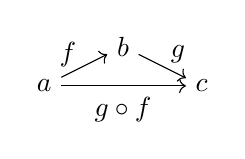
\begin{tikzpicture}
			\node (0) at (-1, 0) {$a$};
			\node (1) at (0, 0.5) {$b$};
			\node (2) at (1, 0) {$c$};
			\node (3) at (-0.7, 0.4) {$f$};
			\node (3) at (0.7, 0.4) {$g$};
			\node (3) at (0, -0.3) {$g\circ f$};
			\draw [->] (0) to (1);
			\draw [->] (1) to (2);
			\draw [->] (0) to (2);
			\end{tikzpicture}
		\end{center}
		\item For any object $a$ an identity morphism $id_a: a \rightarrow a$ 
	\end{itemize}
	Satisfying the following axioms:
	\begin{equation*}
		h \circ (g \circ f) = (h \circ g) \circ f \quad f \circ id_a = f = id_b \circ f
	\end{equation*}
	
\end{definition}
\begin{center}
	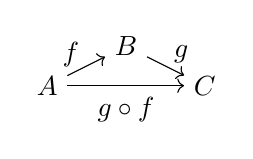
\begin{tikzpicture}
	\node (0) at (-1, 0) {$A$};
	\node (1) at (0, 0.5) {$B$};
	\node (2) at (1, 0) {$C$};
	\node (3) at (-0.7, 0.4) {$f$};
	\node (3) at (0.7, 0.4) {$g$};
	\node (3) at (0, -0.3) {$g\circ f$};
	\draw [->] (0) to (1);
	\draw [->] (1) to (2);
	\draw [->] (0) to (2);
	\end{tikzpicture}
\end{center}
The commutativity of the above diagram is a statement about $\cat$, and it has exactly the same information to its dual diagram. Where objects are one-dimensional wires and morphisms are (zero dimensional) boxes:
\begin{center}
	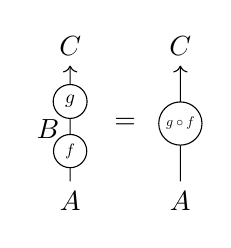
\begin{tikzpicture}[scale=0.7]
	\node (0) at (-1, -1.4) {$A$};
	\node (1) at (-1.4, -0.1) {$B$};
	\node (2) at (-1, 1.4) {$C$};
	\node (3) at (1, -1.4) {$A$};
	\node (4) at (1, 1.4) {$C$};
	\node[scale=0.6,draw,circle] (5) at (-1, -0.5) {$f$};
	\node[scale=0.7,draw,circle] (6) at (-1, 0.4) {$g$};
	\node[scale=0.5,draw,circle] (7) at (1, 0) {$g\circ f$};
	\node (8) at (0, 0) {$=$};
	\draw (0) to (5);
	\draw (5) to (6);
	\draw [->] (6) to (2);
	\draw (3) to (7);
	\draw [->] (7) to (4);
	\end{tikzpicture}
\end{center}
We will mainly use this second diagrammatic language in this work. When $\cat$ is just a category we only have one way of composing morphisms and the language is one dimensional.
\begin{example}
	Examples of categories are: $Sets$ of sets and functions, $FSets$ of finite sets and functions, $Rel$ of sets and relations, $Vect_k$ of vector spaces over $k$ and linear maps and $FVect_k$ of finite dimensional vector spaces and linear maps.
\end{example}
Category theory is a really good language for talking about equivalences and relationships between structures. This is achieved with the following tools.
\begin{definition}[Functor]
	A functor $F:\mathcal{C} \rightarrow \mathcal{D}$ is a mapping that
	\begin{itemize}
		\item associates an object $F(X)$ of $\mathcal{D}$ to each object $X$ of $\mathcal{C}$.
		\item associates to each morphism $f:X \rightarrow Y$ a morphism $F(f): F(X) \rightarrow F(Y)$ such that $F(id_X)=id_Y$ and $F(g\circ f)= F(g)\circ F(f)$ for all morphisms $f:X \rightarrow Y$ and $g:Y \rightarrow Z$.
	\end{itemize}
\end{definition}
For instance there is a functor $Q: Sets \rightarrow Vect_k$ called `1st quantization' and taking a set to the free vector space generated by that set.
Given two functors with matching source and target we can have natural transformations between them
\begin{definition}[Natural Transformation]
	Given categories $\cat$ and $\mathcal{D}$ and functors $F,G:\cat \rightarrow \mathcal{D}$ a natural transformation $\alpha: F \Rightarrow G$ is an assignment to every object $a$ in $\cat$ of a morphism $\alpha_a:F(a) \rightarrow G(a)$ in $\mathcal{D}$ such that for each morphism $f:a \rightarrow b$, the following commutes:
	\begin{center}
		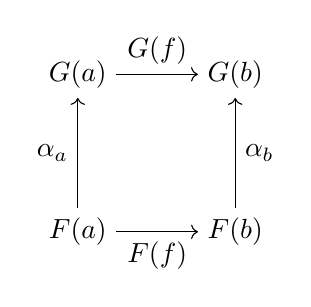
\begin{tikzpicture}[scale=2]
		\node (0) at (0,0) {$F(a)$};
		\node (1) at (0,1) {$G(a)$};
		\node (3) at (1,0) {$F(b)$};
		\node (4) at (1,1) {$G(b)$};
		\draw [->] (0)--(1) node[midway,left] {$\alpha_a$};
		\draw [->] (3)--(4) node[midway,right] {$\alpha_b$};
		\draw [->] (0)--(3) node[midway,below] {$F(f)$};
		\draw [->] (1)--(4) node[midway,above] {$G(f)$};
		\end{tikzpicture}
	\end{center}
	A natural isomorphism is a natural transformation such that all components are isomorphisms.
\end{definition}
%%%MONOIDAL CATEGORIES:
Recall that a monoid is a triple $(X, \times, 1)$ where $X$ is a set, $1 \in X$ and $\times$ is an associative and unital multiplication on $X$. The notion of a monoidal category is the categorification of a monoid. Elements of the set are replaced by objects in a category $\mathcal{C}$, multiplication by a bifunctor $\otimes: \mathcal{C} \times \mathcal{C} \rightarrow \mathcal{C}$ and the equalities in the unit and association axioms are replaced by natural isomorphisms. In order for this new structure to be well-behaved we will also need to impose compatibility conditions. We obtain the following definition:
\begin{definition}[Monoidal category]
A monoidal category is a category $\mathcal{C}$ equipped with a bifunctor $\otimes: \mathcal{C} \times \mathcal{C} \rightarrow \mathcal{C}$ called tensor product, an object $1$ called unit object, a natural isomorphism
$$ a : -\otimes(- \otimes -) \xRightarrow{\sim} (-\otimes -) \otimes -$$ called associator, a natural isomorphism 
$$\lambda: 1 \otimes (-) \Rightarrow (-)$$ called left unitor and a natural isomorphism
$$ \rho: (-) \otimes 1 \Rightarrow (-)$$
called right unitor. Subject to the following coherence conditions holding for all objects $a,b,c,d$ in $\mathcal{C}$:
\begin{enumerate}
    \item Pentagon axiom: the following diagram commutes
    \begin{center}
    	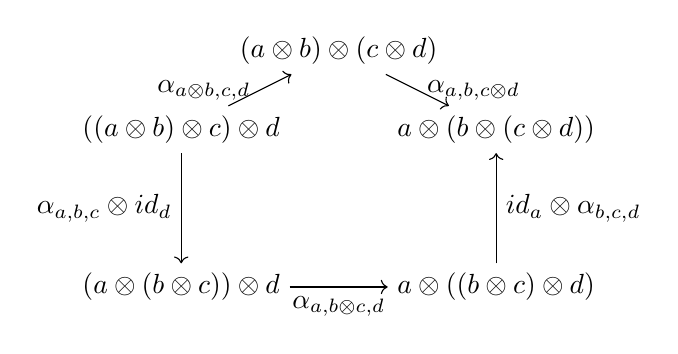
\begin{tikzpicture}[scale=2]
    	\node (0) at (0,0) {$(a\otimes (b \otimes c)) \otimes d$};
    	\node (1) at (0,1) {$((a\otimes b) \otimes c) \otimes d$};
    	\node (2) at (1,1.5) {$(a\otimes b) \otimes (c \otimes d)$};
    	\node (3) at (2,1) {$a\otimes (b \otimes (c \otimes d))$};
    	\node (4) at (2,0) {$a\otimes ((b \otimes c) \otimes d)$};
    	\draw [->] (1)--(2) node[midway,left] {$\alpha_{a \otimes b,c,d}$};
    	\draw [->] (2)--(3) node[midway,right] {$\alpha_{a, b,c \otimes d}$};
    	\draw [->] (1)--(0) node[midway,left] {$\alpha_{a, b,c} \otimes id_d$};
    	\draw [->] (0)--(4) node[midway,below] {$\alpha_{a,b \otimes c,d}$};
    	\draw [->] (4)--(3) node[midway,right] {$id_a \otimes \alpha_{b,c,d}$};
    	\end{tikzpicture}
    \end{center}
    \item Triangle identity: the following diagram commutes
    \begin{center}
    	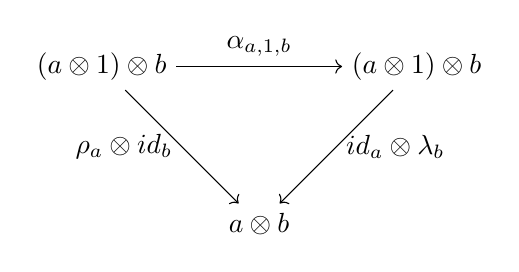
\begin{tikzpicture}[scale=2]
    	\node (0) at (0,0) {$(a\otimes 1) \otimes b$};
    	\node (1) at (2,0) {$(a\otimes 1) \otimes b$};
    	\node (2) at (1,-1) {$a\otimes b$};
    	\draw [->] (0)--(1) node[midway,above] {$\alpha_{a ,1,b}$};
    	\draw [->] (1)--(2) node[midway,right] {$id_a \otimes \lambda_b$};
    	\draw [->] (0)--(2) node[midway,left] {$\rho_a \otimes id_b$};
    	\end{tikzpicture}
    \end{center}
\end{enumerate}
\end{definition}
Let us give three important examples of monoidal categories.
\begin{example}
The category $Sets$ of sets and functions is monoidal with the cartesian product $\times$ as bifunctor and the singleton set as unit object.\\
The category $Vect_k$ of finite dimensional vector spaces over a field $k$ is monoidal with the usual tensor product $\otimes$ and the one dimensional vector space $k$ as unit object.\\
The category $Rel$ of sets and relations is monoidal with the cartesian product $\times$ and the singleton as unit object.
\end{example}
The more structure comes with a category the more complicated diagrams we can draw. Monoidal categories have a two-dimensional diagrammatic language. The presence of unitors and associators and the conditions they satisfy make sure that this graphical language is well behaved. This is known as the coherence theorem for monoidal categories and can be found in \cite{MacLane71}. It says that any well formed diagram in a monoidal category, made up of associators and unitors commutes. When the associators are trivial morphisms (i.e identity morphisms) we say the category is strict monoidal. It is known that every monoidal category is equivalent to a strict one \cite{MacLane71}, but it is sometimes useful to take associators into account as we will see in our discussion on permutational quantum computation.\\
We write the tensor of two morphisms $f \otimes g : A \otimes B \rightarrow C \otimes D$ simply putting them side by side:
\begin{center}
	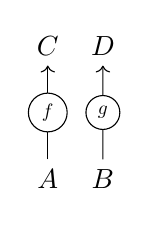
\begin{tikzpicture}[scale=0.7]
	\node (0) at (0, -1.2) {$A$};
	\node (1) at (1, -1.2) {$B$};
	\node (2) at (0, 1.2) {$C$};
	\node (3) at (1, 1.2) {$D$};
	\node[scale=0.7,draw,circle] (5) at (0, 0) {$f$};
	\node[scale=0.7,draw,circle] (6) at (1, 0) {$g$};
	\draw (0) to (5);
	\draw [->] (5) to (2);
	\draw (1) to (6);
	\draw [->] (6) to (3);
	\end{tikzpicture}
\end{center}
In our diagrams we can picture the unit $I$ of the tensor as the plane on which we are drawing. Indeed we could imagine drawing as many copies as we wanted of $id_I$ on the previous diagram to obtain obtain an equivalent diagram as $id_I \otimes f = f$ for any morphism $f$. So really the identity on $I$ is just the empty diagram which we can stick next to any diagram we like.
\begin{definition}[States and costates]
	Given a system $A$, a state of is a morphism $1 \rightarrow A$. A costate (or effect) of $A$ is a morphism $A \rightarrow 1$. In the diagrammatic language we draw states and costates respectively:
	\begin{center}
		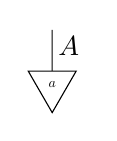
\begin{tikzpicture}[scale=0.7]
		\node[scale=0.5,buffer] (1) {$a$}; 
		\node (2) at (0.3,0.7) {$A$};
		\draw (1)--(0,1);
		\end{tikzpicture}
		\quad \quad
		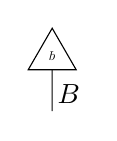
\begin{tikzpicture}[scale=0.7]
		\node[scale=0.5,buffer,rotate=180] (1) at (0,0) {$q$}; 
		\node (2) at (0.3,-0.7) {$B$};
		\draw (1)--(0,-1);
		\end{tikzpicture}
	\end{center}
			
	
\end{definition}


%%%DIAGRAMS:
\begin{remark}
	It is perhaps useful to understand monoidal categories as degenerate 2-categories. Although this viewpoint requires one additional initial step of abstraction (the definition of a 2-category), it gives us the diagrammatic language for monoidal categories for free. For the rigorous definition of a 2-category we refer to [BAEZ], for our purposes we will only need the intuition. A 2-category is a collection of objects with 1-arrows between them and 2-arrows between the 1-arrows. Note that there are two ways of composing the 2-arrows:
	\begin{itemize}
		\item vertical composition:
		\begin{center}
			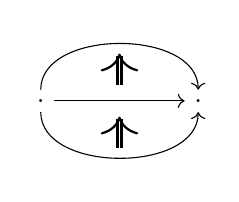
\begin{tikzpicture}
			\node (0) at (0,0) {.};
			\node (1) at (2,0) {.};
			\draw[->] (0) to (1);
			\draw[->, bend right=90] (0) to (1);
			\draw[->, bend left=90] (0) to (1);
			\draw[double, thick, ->] (1,-0.6) to (1,-0.2);
			\draw[double, thick, ->] (1,0.2) to (1,0.6);
			\end{tikzpicture}
		\end{center}
		\item parallel composition:
		\begin{center}
			\begin{tikzpicture}
			\node (0) at (0,0) {.};
			\node (1) at (2,0) {.};
			\node (2) at (4,0) {.};
			\draw[->, bend right=40] (0) to (1);
			\draw[->, bend left=40] (0) to (1);
			\draw[->, bend right=40] (1) to (2);
			\draw[->, bend left=40] (1) to (2);
			\draw[double, thick, ->] (1,-0.2) to (1,0.2);
			\draw[double, thick, ->] (3,-0.2) to (3,0.2);
			\end{tikzpicture}
		\end{center}
	\end{itemize}
	Taking the dual of the above diagrams we obtain the diagrammatic language. Monoidal categories are 2-categories with only one 0-object called $1$. We can think of the 0-object as the underlying plane, wires carry systems (1-arrows), boxes are morphisms (2-arrows). We recover the given definition of monoidal category by calling 1-arrow objects, and 2-arrows morphisms. The unit object $1$ is then the identity 1-arrow $1 \rightarrow 1$ which is simply denoted $1$.
\end{remark}
 
\begin{example}
The cartesian product in $Sets$ $A \times B$ of sets $A$ and $B$, satisfies the universal properties of a categorical product, in the sense that we have projections $p_1$ and $p_2$ such that if $f$ and $g$ are maps from some set $C$ there is a unique function $h$ making the following diagram commute:
\begin{center}
	\begin{tikzpicture}
	\node (0) at (-1, 0) {$A$};
	\node (1) at (1, 0) {$B$};
	\node (2) at (0, 1) {$A \times B$};
	\node (3) at (0, -1) {$C$};
	\node (4) at (0.2, 0) {$h$};
	\node (5) at (-0.8, 0.6) {$p_1$};
	\node (6) at (0.8, 0.6) {$p_2$};
	\node (7) at (-0.8, -0.6) {$f$};
	\node (8) at (0.8, -0.6) {$g$};
	\draw [->] (2) to (0);
	\draw [->] (2) to (1);
	\draw [->] (3) to (1);
	\draw [->] (3) to (0);
	\draw [->] (3) to (2);
	\end{tikzpicture}
\end{center}
Because of this property all states of $(Sets,\times)$ are separable. This category is the ambient Cartesian world of classical physics.
\end{example}
\begin{example}
In $Vect_k$ states are vectors and costates are functionals. Note that the diagrammatic notation provides a two-dimensional generalisation of Dirac's notation. The category $Hilb$ of Hilbert spaces and linear maps is monoidal when equipped with the usual tensor product $\otimes$. Note that $\otimes$ is not a categorical product, and in fact we can have entangled states. Quantum mechanics is based on $(Hilb, \otimes)$ \cite{Vicary12}.
\end{example}
\begin{definition}[Scalars]
Scalars in a monoidal category are morphisms $1 \rightarrow 1$.
\end{definition}
The category $Sets$ has only one scalar. $Rel$ has two scalars forming the cyclic group $\mathbb{Z}_2$ under composition. $Vect_k$ has scalars from $k$. Given a vector and a functional we obtain a scalar by composing them analogously to Dirac's formalism.
\begin{definition}[BMC]
	A braided monoidal category is a monoidal category $\mathcal{C}$ equipped with a natural isomorphism $B_{a,b} : a \otimes b \rightarrow b \otimes a$ called braiding, subject to the following compatibility conditions (called hexagon equations):
	\begin{center}
		\begin{tikzpicture}[scale=2]
		\node (0) at (-1,0) {$(a\otimes b) \otimes c$};
		\node (1) at (-0.5,1) {$a\otimes (b \otimes c)$};
		\node (2) at (1.5,1) {$(b\otimes c)\otimes a$};
		\node (3) at (2,0) {$b\otimes (c\otimes a)$};
		\node (4) at (-0.5,-1) {$(b\otimes a)\otimes c$};
		\node (5) at (1.5,-1) {$b\otimes (a\otimes c)$};
		\draw [->] (0)--(1) node[midway,left] {$\alpha_{a,b,c}$};
		\draw [->] (1)--(2) node[midway,above] {$B_{a,b \otimes c}$};
		\draw [->] (2)--(3) node[midway,right] {$\alpha_{b,c,a}$};
		\draw [->] (0)--(4) node[midway,left] {$B_{a,b} \otimes id_c$};
		\draw [->] (4)--(5) node[midway,below] {$\alpha_{b,a,c}$};
		\draw [->] (5)--(3) node[midway,right] {$id_b \otimes B_{a,c}$};
		\end{tikzpicture}
	\end{center}
	\begin{center}
		\begin{tikzpicture}[scale=2]
		\node (0) at (-1,0) {$a\otimes (b \otimes c)$};
		\node (1) at (-0.5,1) {$(a\otimes b) \otimes c$};
		\node (2) at (1.5,1) {$c\otimes (a\otimes b)$};
		\node (3) at (2,0) {$(c\otimes a)\otimes b$};
		\node (4) at (-0.5,-1) {$a\otimes (c\otimes b)$};
		\node (5) at (1.5,-1) {$(a\otimes c)\otimes b$};
		\draw [->] (0)--(1) node[midway,left] {$\alpha_{a,b,c}$};
		\draw [->] (1)--(2) node[midway,above] {$B_{a\otimes b,c}$};
		\draw [->] (2)--(3) node[midway,right] {$\alpha_{c,a,b}$};
		\draw [->] (0)--(4) node[midway,left] {$id_a \otimes B_{b,c}$};
		\draw [->] (4)--(5) node[midway,below] {$\alpha_{a,c,b}$};
		\draw [->] (5)--(3) node[midway,right] {$B_{a,c} \otimes id_b$};
		\end{tikzpicture}
	\end{center}
	
\end{definition}
In the diagrammatic language this means we have braidings:
\begin{center}
	\begin{tikzpicture}[scale=0.9, whit/.style={draw,regular polygon,
		regular polygon sides=4,fill=white}, black/.style={draw,regular polygon, regular polygon sides=4,fill=black}]
	\node (0) at (0.5,0.5) {};
	\node (1) at (-0.1,-0.4) {$A$};
	\node (2) at (1.1,-0.4) {$B$};
	\draw (0,1) to (1,0);
	\draw (0,0) to (0);
	\draw (0) to (1,1);
	\end{tikzpicture}
	\begin{tikzpicture}[scale=0.9, whit/.style={draw,regular polygon,
		regular polygon sides=4,fill=white}, black/.style={draw,regular polygon, regular polygon sides=4,fill=black}]
	\node (0) at (0.5,0.5) {};
	\node (1) at (-0.1,-0.4) {$B$};
	\node (2) at (1.1,-0.4) {$A$};
	\draw (0,0) to (1,1);
	\draw (0,1) to (0);
	\draw (0) to (1,0);
	\end{tikzpicture}
\end{center}
for any $A$ and $B$, satifying:
\begin{equation}
\begin{gathered}
\begin{tikzpicture}[scale=0.6, whit/.style={draw,regular polygon,
	regular polygon sides=4,fill=white}, black/.style={draw,regular polygon, regular polygon sides=4,fill=black}]
\node (0) at (0.5,0.5) {};
\node (1) at (-0.1,-0.4) {$A$};
\node (2) at (1.1,-0.4) {$B$};
\node (3) at (0.5,1.5) {};
\draw (1,0)--(0,1)--(1,2);
\draw (0,0)--(0)--(1,1)--(3)--(0,2);
\end{tikzpicture}
\end{gathered}
\, = \,
\begin{gathered}
\begin{tikzpicture}[scale=0.6, whit/.style={draw,regular polygon,
	regular polygon sides=4,fill=white}, black/.style={draw,regular polygon, regular polygon sides=4,fill=black}]
\node (1) at (0,-0.4) {$A$};
\node (2) at (0.9,-0.4) {$B$};
\draw (0.8,0)--(0.8,2);
\draw (0.1,0)--(0.1,2);
\end{tikzpicture}
\end{gathered}
\quad;\quad
\begin{gathered}
\begin{tikzpicture}[scale=0.6, whit/.style={draw,regular polygon,
	regular polygon sides=4,fill=white}, black/.style={draw,regular polygon, regular polygon sides=4,fill=black}]
\node (0) at (0.5,0.5) {};
\node (1) at (-0.1,-0.4) {$B$};
\node (2) at (1.1,-0.4) {$A$};
\node (3) at (0.5,1.5) {};
\draw (1,0)--(0)--(0,1)-- (3)--(1,2);
\draw (0,0)--(1,1)--(0,2);
\end{tikzpicture}
\end{gathered}
\, = \,
\begin{gathered}
\begin{tikzpicture}[scale=0.6, whit/.style={draw,regular polygon,
	regular polygon sides=4,fill=white}, black/.style={draw,regular polygon, regular polygon sides=4,fill=black}]
\node (1) at (0,-0.4) {$B$};
\node (2) at (0.9,-0.4) {$A$};
\draw (0.8,0)--(0.8,2);
\draw (0.1,0)--(0.1,2);
\end{tikzpicture}
\end{gathered}
\end{equation}
The compatibility conditions are obvious statements in the diagrammatic calculus, for instance the first hexagon equation just says:
\begin{equation}
\begin{gathered}
\begin{tikzpicture}[scale=0.6]
\node (0) at (0.5,0.5) {};
\node (1) at (-0.1,-0.4) {$A$};
\node (2) at (1.1,-0.4) {$B$};
\node (3) at (2.1,-0.4) {$C$};
\node (4) at (1.5,2.5) {};
\draw (0,0)--(1,1)--(1,2)--(2,3);
\draw (1,0)--(0)--(0,1)--(0,3);
\draw (2,0)--(2,2)--(4)--(1,3);
\end{tikzpicture}
\end{gathered}
\, = \,
\begin{gathered}
\begin{tikzpicture}[scale=0.6]
\node (0) at (1.3,2.2) {};
\node (1) at (0.4,-0.4) {$A$};
\node (2) at (1.5,-0.4) {$B$};
\node (3) at (2.2,-0.4) {$C$};
\node (4) at (1.5,2.5) {};
\draw (0.5,0)--(0.5,1.5)--(1,2)--(2,3);
\draw (1.7,0)--(1.7,1.7)--(0)--(0.5,3);
\draw (2,0)--(2,2)--(4)--(1,3);
\end{tikzpicture}
\end{gathered}
\end{equation}
Both $Sets$ and $Hilb$ are examples of symmetric monoidal categories in the following sense.
\begin{definition}[SMC]
	A braided monoidal category is symmetric if the braiding $B_{a,b}$ satisfies $$B_{a,b} \circ B_{b,a} = id_{a\otimes b}$$
	For all objects $a,b$
\end{definition}
In a SMC the braiding is called symmetry morphism and is denoted
\begin{center}
	\symAB	
\end{center}
It satisfies:
\symequation
We will now describe some new classes of examples of monoidal categories. These are of a different nature to the categories we have seen so far.
\begin{definition}[PROPs]
	A $PROP$ (products and permutations category) is a strict symmetric monoidal category where every object is of the form $x^{\otimes n}$ for a single object $x$ and $n \geq 0$.
\end{definition}
This means that we are only allowed one type of wire when drawing diagrams about $PROPs$ but we can use as many copies as we like and we can make swaps with them. Categories satisfying these properties are useful syntactic tools as we will see.
One way to think of a $PROP$ $A$ is as an abstract algebraic structure carrying some axioms, we can then instantiate those axioms in some other symmetric monoidal category $\mathcal{C}$ by considering symmetric monoidal functors $F: A \rightarrow \mathcal{C}$. We call such functors algebras or models of $A$ in $\mathcal{C}$. If $A$ is defined in terms of generators and relations (as is most often done), the choice of such functor corresponds to the choice of one object from $\mathcal{C}$ and morphisms on that object respecting the defining relations of $A$. On its own $A$ has no clear interpretation, it just defines a syntax, but if $\mathcal{C}$ is a semantic category (i.e one with a clear interpretation) then $F$ is a `filling' of the syntax with meaning. This reasoning was first proposed in Lawvere's Phd thesis in 1963 \cite{Lawvere63}.\\
It will sometimes be useful to drop the `permutational' structure of $PROPs$.
\begin{definition}[PRO]
	A $PRO$ (products category) is a strict monoidal category where every object is of the form $x^{\otimes n}$ for a single object $x$ and $n \geq 0$.
\end{definition}
The semantic categories we will consider the most are $Sets$ and $Hilb$. One important difference between them is that $Hilb$ exhibits duality.
\begin{definition}[Rigidity]
	Let $\mathcal{C}$ be a monoidal category and $A\in obj(\mathcal{C})$. A left-dual of $A$ is an object $A^*$ with morphisms
	\begin{center}
		\cupA \, \capA
	\end{center}
	Satisfying the snake equations:
	\snake
	\snakestar
	If every object has a left-dual, we say that $\mathcal{C}$ is left-rigid.
	Similarly we can define right-duals and right-rigid categories by interchanging the roles of $A$ and $A^\star$ in the definition.
\end{definition}
Given a (left/right) rigid structure we can define (left/right)transpose as follows.
\begin{definition}[Transpose]
	Given a (left/right) rigid category $\cat$ and any process $f:A \rightarrow B$ the (left/right) transpose $f^*$ (or left transpose $f^l$, right transpose $f^r$ if it is not clear from context) is:
	\begin{equation}
	\begin{gathered}
	\begin{tikzpicture}
		\node[draw, trapezium, trapezium angle=70, shape border rotate=180] (0) at (0,0) {$f$};
		\draw[->] (0) to (0,-0.7);
		\draw[->] (0,0.7) to (0);
	\end{tikzpicture}
	\end{gathered}
	\, = \,
	\begin{gathered}
	\begin{tikzpicture}
	\node[draw, trapezium, trapezium angle=70,] (0) at (0,0) {$f$};
	\draw[->] (0,-0.7)--(0)--(0,0.7);
	\draw[bend right=90] (0,0.7) to (-0.7,0.7);
	\draw[->] (-0.7,0.7) to (-0.7,-0.7);
	\draw[bend right=90] (0,-0.7) to (0.7,-0.7);
	\draw[->] (0.7,0.7) to (0.7,-0.7);
	\end{tikzpicture}
	\end{gathered}	
	\end{equation}
\end{definition}
\begin{definition}[Trace]
	In a symmetric monoidal category $\cat$, if $A$ has a left dual $A^\star$, the trace of some morphism $f:A \rightarrow A$ is defined as the following scalar:
	\begin{center}
	\begin{tikzpicture}[scale=0.7]
	\node[scale=0.7, draw, trapezium, trapezium angle=70,] (0) at (0,0) {$f$};
	\draw[->] (0,-0.7)--(0)--(0,0.7);
	\draw[bend right=90] (0,0.7) to (-0.7,0.7);
	\draw[->] (-0.7,0.7) to (-0.7,-0.7);
	\draw[bend left=90] (0,-1.3) to (-0.7,-1.3);
	\draw[->] (-0.7,-0.7) to (0,-1.3);
	\draw[->] (0,-0.7) to (-0.7,-1.3);
	\end{tikzpicture}	
	\end{center}
\end{definition}

%%%%%%%%%%%%%%%%%%%%%%%%%%%%%%%%%%%%%%%%%%%%%%%%%%%%%%%%%%%%%%%%%%%%%%%%%%%%%%%%%%%%%%%%%%%%%%%%%%%%%%%%%%%%%%%%%%%%%%%%%%%%%%%%%%%%%%%%%%%%%%%%%%%%%%%%%%%%%%%%%%%%%%%%%%%%%%%%%%%%%%%%%%%%%%%%%%%%%%%%%%%%%%%%%%%%%%%%%%%%%%%%%%%%%%%%%%%%%%%%%%%%%%%%%%%%%%%%%%%%%%%%%%%%%%%%%%%%%%%%%%%%%%%%%%%%%%%%%%%%%%%%%%%%%%%%%%%%%%%%%%%%%%%%%%%%%%%%%%%%%%%%%%%%%%%%%%%%%%%%%%

\subsection{Hopf Algebras}
Now that we have set in place a diagrammatic machinery based on monoidal categories, let us make use of it. In this section we will meet some mathematical structures which have been used by mathematicians to describe symmetry. The notion of Hopf algebras is a powerful generalization of that of a group. Since their discovery in the 1940s, Hopf algebras have been used in various fields of pure mathematics (such as number theory, algebraic geometry, and representation theory) and have found applications in Quantum mechanics. Most of the results of this section can be found in \cite{Majid95}. 
\begin{definition}[Monoid]
	$\Delta$ is a $PRO$ generated by morphisms (\mult, \unit) satisfying associativity: \associativity
	and the unit law: \unitlaw
\end{definition}
Models of $\Delta$ in monoidal categories are called monoids and they are very well known, examples include the natural numbers under addition, lists of some alphabet under concatenation and any group. Taking the opposite category $\Delta^{op}$ corresponds to flipping all the diagrams.
\begin{definition}[Comonoid]
	$\Delta^{op}$ is a $PRO$ generated (\comult, \counit) satisfying coassociativity: \coassociativity and the counit law: \counitlaw
\end{definition}
Models of these are comonoids, the most common example is the copy map on any set with `delete' as counit.
Monoids and comonoids are simple structures that we can stick together to form more complicated ones. Bialgebras arise from one type of interaction of a monoid and comonoid.
\begin{definition}[Bialg]
	$Bialg$ is a $PROP$ generated by (\mult, \unit, \comult, \counit), where \mult and \unit form a monoid, \comult and \counit a comonoid and the morphisms additionally satisfy the following laws:
	\bialgebralaw
	\copylaw
	\cocopylaw
	\begin{equation}
		\begin{gathered}
		\begin{tikzpicture}[scale=0.7]
			\node[scale=0.5,draw,circle,fill=black] (0) at (0,0) {};
			\node[scale=0.5,draw,circle,fill=white] (1) at (0,1) {};
			\draw (0) to (1);
		\end{tikzpicture}
		\end{gathered}
		\, = \,
	\end{equation}
	Where the empty diagram is the identity on the tensor unit.
\end{definition}
Models of $Bialg$ in $Vect$ are bialgebras. We leave examples for later as we are now ready to introduce one of the main topics of this thesis.
\begin{definition}[Hopf]
	$Hopf$ is a $PROP$ generated by (\mult , \unit , \comult , \counit , \antipode). Where (\mult, \unit, \comult, \counit) is a bialgebra and the antipode $S$ satisfies the Hopf law:
	\hopflaw
\end{definition}
We will argue that $Hopf$ is a good syntax to talk about symmetry. Let us start by  instantiating $G: Hopf \rightarrow Sets$. This corresponds to choosing a set $G$, with a binary function $G \times G \rightarrow G$ (or multiplication) with a unit. Using the counit rule it is easy to see that the comultiplication in $Sets$ must be the copy map $g \mapsto (g,g)$ so that the antipode is the morphism $g \mapsto g^{-1}$ and $G$ forms a group. Since the $19^{th}$ century groups have been used by mathematicians and physicists to describe symmetry.
\begin{example}[Finite groups]
	We will only make use of the following classes of finite groups:
	\begin{itemize}
		\item $\mathbb{Z}_n$ the cyclic group with $n$ elements.
		\item $S_n$ the symmetric group, can be seen as the group of permutations of a set with $n$ elements, has order $n!$. $S_3$ is the smallest non-abelian group up to isomorphism.  
	\end{itemize}
\end{example}
\begin{example}[Groups of matrices]
	Here we will fix some notation on the infinite groups of matrices we will meet. All matrices we will consider are over the complex numbers. $GL(n)$ is the group of invertible $n$ by $n$ complex matrices. $U(n)$ is the group of unitary $n \times n$ matrices (i.e such that $U^{\dagger}U = UU^\dagger = I$). The special unitary group $SU(n)$ is the subgroup of $U(n)$ consisting of matrices with determinant $1$. The representation theory of $SU(n)$ is widely used in particle physics, for instance representations of $SU(2)$ model the behaviour of spin-$\frac{1}{2}$ particles. 
\end{example}
If we take a model of $H:Hopf \rightarrow Vect$ we obtain what is known as a Hopf Algebra.
\begin{example}[Group algebras]
	If $G$ is a group with unit $e$, the group algebra $\mathbb{C}G$ (of dimension $|G|$) is a hopf algebra with multiplication linearly generated by $\ket{g}\otimes \ket{h} \rightarrow \ket{gh}$, unit $\ket{e}$, comultplication generated by $\ket{g} \rightarrow \ket{g} \otimes \ket{g}$ and counit $\sum_g \bra{g}$.
\end{example}
The previous example gives the usual definition of a group algebra which, for finite sets and finite dimensional vector spaces is just the composition $Q \circ G$ (as shown in the diagram) where $Q$ is the 1st quantization functor. It is easy to see that $Q$ preserves the monoidal structure as well as the symmetry morphisms (we say $Q$ is a symmetric monoidal functor) so that the composition is also symmetric monoidal and $Q \circ G$ is a model of $Hopf$.
\begin{center}
	\begin{tikzpicture}
	\node (0) at (-1, 0) {$FSets$};
	\node (1) at (1, 0) {$FVect$};
	\node (2) at (0, 1) {$Hopf$};
	\node (5) at (-0.8, 0.6) {$G$};
	\node (6) at (0.8, 0.6) {$\mathbb{C}G$};
	\node (7) at (0, -0.3) {$Q$};
	\draw [->] (2) to (0);
	\draw [->] (2) to (1);
	\draw [->] (0) to (1);
	\end{tikzpicture}
\end{center}
In this case the comultiplication in $Hilb$ is the linearisation of the copy map (the copy map on some basis extended linearly to the whole Hilbert space) which is co-commutative. For a general $H:Hopf \rightarrow Vect$ this doesn't have to be the case. Hopf algebras provide a broader framework to talk about symmetry, as we can have non co-commutative Hopf algebras. We can see it as a quantization of the notion of symmetry, it will allow us to describe symmetries of quantum systems. Physically we will see that Hopf algebras allow to talk about local symmetries and exchange statistics on the same footing \cite{Slingerland02}. In particular if the Hopf algebra is not cocommutative the exchange statistics can be highly non-trivial, in which case they will describe the symmetries of anyons.
The following two propositions are simple but important results about the antipode of a hopf algebra.
\begin{proposition}
	The antipode of a Hopf algebra is unique. It follows that being a Hopf algebra is a property of bialgebras. 
\end{proposition}
\begin{proof}
	Suppose $S$ and $S'$ are two antipodes for some Hopf algebra, then:
	\begin{equation}
	\begin{gathered}
	\begin{tikzpicture}[squr/.style={draw,regular polygon,
		regular polygon sides=4,fill=white}]
	\node[squr,scale=0.5] (0) at (0,0.5) {$S$};
	\draw (0,-0.5) to (0);
	\draw (0,1.5) to (0);
	\end{tikzpicture}
	\end{gathered}
	\, = \,
	\begin{gathered}
	\begin{tikzpicture}[squr/.style={scale=0.5,draw,regular polygon,
		regular polygon sides=4,fill=white}]
	\node[scale=0.5,draw,circle,fill=white] (0) at (0,0) {};
	\node[scale=0.5,draw,circle,fill=black] (1) at (0,1) {};
	\node[squr] (2) at (0.5,0.5) {$S$};
	\node[scale=0.5,draw,circle,fill=white] (3) at (-0.3,0.3) {};
	\node[scale=0.5,draw,circle,fill=black] (4) at (-0.3,0.7) {};
	\draw[bend left] (0) to (3);
	\draw[bend left] (4) to (1);
	\draw[bend right] (0) to (2);
	\draw[bend right] (2) to (1);
	\draw (0,-0.5) to (0);
	\draw (0,1.5) to (1);
	\end{tikzpicture}
	\end{gathered}
	\, = \,
	\begin{gathered}
	\begin{tikzpicture}[squr/.style={scale=0.5,draw,regular polygon,
		regular polygon sides=4,fill=white}]
	\node[scale=0.5,draw,circle,fill=white] (0) at (0,0) {};
	\node[scale=0.5,draw,circle,fill=black] (1) at (0,1) {};
	\node[squr] (2) at (0.5,0.5) {$S$};
	\node[scale=0.5,draw,circle,fill=white] (3) at (-0.3,0.2) {};
	\node[scale=0.5,draw,circle,fill=black] (4) at (-0.3,0.8) {};
	\node[squr, scale=0.5] (5) at (-0.5,0.5) {$S'$};
	\draw[bend left] (0) to (3);
	\draw[bend left] (4) to (1);
	\draw[bend right] (0) to (2);
	\draw[bend right] (2) to (1);
	\draw[bend left] (3) to (5);
	\draw[bend left] (5) to (4);
	\draw[bend right=70] (3) to (4);
	\draw (0,-0.5) to (0);
	\draw (0,1.5) to (1);
	\end{tikzpicture}
	\end{gathered}
	\, = \,
	\begin{gathered}
	\begin{tikzpicture}[squr/.style={scale=0.5,draw,regular polygon,
		regular polygon sides=4,fill=white}]
	\node[scale=0.5,draw,circle,fill=white] (0) at (0,0) {};
	\node[scale=0.5,draw,circle,fill=black] (1) at (0,1) {};
	\node[squr,scale=0.8] (2) at (-0.5,0.5) {$S'$};
	\node[scale=0.5,draw,circle,fill=white] (3) at (0.3,0.2) {};
	\node[scale=0.5,draw,circle,fill=black] (4) at (0.3,0.8) {};
	\node[squr, scale=0.5] (5) at (0.5,0.5) {$S$};
	\draw[bend right] (0) to (3);
	\draw[bend right] (4) to (1);
	\draw[bend left] (0) to (2);
	\draw[bend left] (2) to (1);
	\draw[bend right] (3) to (5);
	\draw[bend right] (5) to (4);
	\draw[bend left=70] (3) to (4);
	\draw (0,-0.5) to (0);
	\draw (0,1.5) to (1);
	\end{tikzpicture}
	\end{gathered}
	\, = \,
	\begin{gathered}
	\begin{tikzpicture}[squr/.style={scale=0.5,draw,regular polygon,
		regular polygon sides=4,fill=white}]
	\node[scale=0.5,draw,circle,fill=white] (0) at (0,0) {};
	\node[scale=0.5,draw,circle,fill=black] (1) at (0,1) {};
	\node[squr,scale=0.8] (2) at (-0.5,0.5) {$S'$};
	\node[scale=0.5,draw,circle,fill=white] (3) at (0.3,0.3) {};
	\node[scale=0.5,draw,circle,fill=black] (4) at (0.3,0.7) {};
	\draw[bend right] (0) to (3);
	\draw[bend right] (4) to (1);
	\draw[bend left] (0) to (2);
	\draw[bend left] (2) to (1);
	\draw (0,-0.5) to (0);
	\draw (0,1.5) to (1);
	\end{tikzpicture}
	\end{gathered}
	\, = \,
	\begin{gathered}
	\begin{tikzpicture}[squr/.style={draw,regular polygon,
		regular polygon sides=4,fill=white}]
	\node[squr,scale=0.4] (0) at (0,0.5) {$S'$};
	\draw (0,-0.5) to (0);
	\draw (0,1.5) to (0);
	\end{tikzpicture}
	\end{gathered}
	\end{equation}
\end{proof}

\begin{proposition}
	The antipode is an anti-(co)algebra homomorphism.
	\begin{equation}
	\begin{gathered}
	\begin{tikzpicture}[scale=0.7, squr/.style={draw,regular polygon,
		regular polygon sides=4,fill=white}]
		\node[scale=0.5, draw, circle, fill=white] (0) at (0,0) {};
		\node[scale=0.5, squr] (1) at (0, -0.6) {$S$};
		\draw (1) to (0);
		\draw (0,-1) to (1);
		\draw[bend left] (0) to (-0.5,1);
		\draw[bend right] (0) to (0.5,1);
	\end{tikzpicture}
	\end{gathered}
	\, = \,
	\begin{gathered}
	\begin{tikzpicture}[scale=0.7, squr/.style={draw,regular polygon,
		regular polygon sides=4,fill=white}]
	\node[scale=0.5, draw, circle, fill=white] (0) at (0,-0.3) {};
	\node[scale=0.5, squr] (1) at (-0.5, 0.6) {$S$};
	\node[scale=0.5, squr] (2) at (0.5, 0.6) {$S$};
	\draw[bend left=70] (0) to (0,0.1);
	\draw[bend right=70] (0) to (0,0.1);
	\draw (0,-1) to (0);
	\draw (1) to (-0.5,1);
	\draw (2) to (0.5,1);
	\draw[bend left] (0,0.1) to (1);
	\draw[bend right] (0,0.1) to (2);
	\end{tikzpicture}
	\end{gathered}
	\quad ; \quad
	\begin{gathered}
	\begin{tikzpicture}[scale=0.7, squr/.style={draw,regular polygon,
		regular polygon sides=4,fill=white}]
	\node[scale=0.5, draw, circle, fill=black] (0) at (0,0) {};
	\node[scale=0.5, squr] (1) at (0, 0.6) {$S$};
	\draw (1) to (0);
	\draw (0,1) to (1);
	\draw[bend right] (0) to (-0.5,-1);
	\draw[bend left] (0) to (0.5,-1);
	\end{tikzpicture}
	\end{gathered}
	\, = \,
	\begin{gathered}
	\begin{tikzpicture}[scale=0.7, squr/.style={draw,regular polygon,
		regular polygon sides=4,fill=white}]
	\node[scale=0.5, draw, circle, fill=black] (0) at (0,0.3) {};
	\node[scale=0.5, squr] (1) at (-0.5, -0.6) {$S$};
	\node[scale=0.5, squr] (2) at (0.5, -0.6) {$S$};
	\draw[bend left=70] (0) to (0,-0.1);
	\draw[bend right=70] (0) to (0,-0.1);
	\draw (0,1) to (0);
	\draw (1) to (-0.5,-1);
	\draw (2) to (0.5,-1);
	\draw[bend right] (0,-0.1) to (1);
	\draw[bend left] (0,-0.1) to (2);
	\end{tikzpicture}
	\end{gathered}
	\end{equation}
\end{proposition}
\begin{proof}
	First note that:
	\begin{equation}
	\begin{gathered}
	\begin{tikzpicture}[scale=0.8, squr/.style={draw,regular polygon,
		regular polygon sides=4,fill=white}]
	\node[scale=0.5, draw, circle, fill=white] (0) at (0,-1) {};
	\node[scale=0.5, draw, circle, fill=white] (1) at (-1,0) {};
	\node[scale=0.5, draw, circle, fill=white] (2) at (1,0) {};
	\node[scale=0.5, draw, circle, fill=black] (3) at (-1,0.5) {};
	\node[scale=0.5, draw, circle, fill=black] (4) at (1,0.5) {};
	\node[scale=0.5, squr] (5) at (-0.7, -0.6) {$S$};
	\draw (0,-1.3) to (0);
	\draw[bend left] (0) to (5);
	\draw[bend right] (0) to (2);
	\draw (5)--(1)--(3)--(-1,1);
	\draw (2)--(4)--(1,1);
	\draw (1) to (4);
	\draw (2) to (3);
	\end{tikzpicture}
	\end{gathered}
	\, = \,
	\begin{gathered}
	\begin{tikzpicture}[scale=0.8, squr/.style={draw,regular polygon,
		regular polygon sides=4,fill=white}]
	\node[scale=0.5, draw, circle, fill=white] (0) at (0,-1) {};
	\node[scale=0.5, draw, circle, fill=white] (1) at (0,0.5) {};
	\node[scale=0.5, draw, circle, fill=black] (2) at (0,0) {};
	\node[scale=0.5, squr] (S) at (-0.5, -0.5) {$S$};
	\draw (0,-1.3) to (0);
	\draw[bend left] (0) to (S);
	\draw[bend left] (S) to (2);
	\draw[bend right=70] (0) to (2);
	\draw (2) to (1);
	\draw[bend left] (1) to (-0.5,1);
	\draw[bend right] (1) to (0.5,1);
	\end{tikzpicture}
	\end{gathered}
	\, = \,
	\begin{gathered}
	\begin{tikzpicture}[scale=0.8, squr/.style={draw,regular polygon,
		regular polygon sides=4,fill=white}]
	\node[scale=0.5, draw, circle, fill=white] (0) at (0,-0.6) {};
	\node[scale=0.5, draw, circle, fill=white] (1) at (0,0.5) {};
	\node[scale=0.5, draw, circle, fill=black] (2) at (0,0) {};
	\draw (0,-1.3) to (0);
	\draw (2) to (1);
	\draw[bend right] (1) to (0.5,1);
	\draw[bend left] (1) to (-0.5,1);
	\end{tikzpicture}
	\end{gathered}
	\, = \,
	\begin{gathered}
	\begin{tikzpicture}[scale=0.8, squr/.style={draw,regular polygon,
		regular polygon sides=4,fill=white}]
	\node[scale=0.5, draw, circle, fill=white] (0) at (0,-0.6) {};
	\node[scale=0.5, draw, circle, fill=black] (1) at (-0.5,0.3) {};
	\node[scale=0.5, draw, circle, fill=black] (2) at (0.5,0.3) {};
	\draw (0,-1.3) to (0);
	\draw (2) to (0.5,1);
	\draw (1) to (-0.5,1);
	\end{tikzpicture}
	\end{gathered}
	\end{equation}
	So that 
	\begin{tikzpicture}[scale=0.4, squr/.style={draw,regular polygon,
		regular polygon sides=4,fill=white}]
	\node[scale=0.5, draw, circle, fill=white] (0) at (0,0) {};
	\node[scale=0.2, squr] (1) at (0, -0.6) {$S$};
	\draw (1) to (0);
	\draw (0,-1) to (1);
	\draw[bend left] (0) to (-0.5,0.5);
	\draw[bend right] (0) to (0.5,0.5);
	\end{tikzpicture}
	is a left convolution inverse to 
	\begin{tikzpicture}[scale=0.4, squr/.style={draw,regular polygon,
		regular polygon sides=4,fill=white}]
	\node[scale=0.5, draw, circle, fill=white] (0) at (0,0) {};
	\draw (0,-1) to (0);
	\draw[bend left] (0) to (-0.5,0.5);
	\draw[bend right] (0) to (0.5,0.5);
	\end{tikzpicture}.\\
	Also:
	\begin{equation}
	\begin{gathered}
	\begin{tikzpicture}[scale=0.8, squr/.style={draw,regular polygon,
		regular polygon sides=4,fill=white}]
	\node[scale=0.5, draw, circle, fill=white] (0) at (0,-1) {};
	\node[scale=0.5, draw, circle, fill=white] (1) at (0.6,-0.8) {};
	\node[scale=0.5, draw, circle, fill=white] (2) at (-0.6,-0.4) {};
	\node[scale=0.5, draw, circle, fill=black] (3) at (0.6,0.7) {};
	\node[scale=0.5, draw, circle, fill=black] (4) at (-0.6,0.7) {};
	\node[scale=0.4, squr] (5) at (0.2, 0) {$S$};
	\node[scale=0.4, squr] (6) at (0.7, 0) {$S$};
	\draw (0,-1.3)--(0)--(1);
	\draw (0)--(2)--(4);
	\draw[bend right, looseness=1.3] (1) to (5);
	\draw[bend left, looseness=1.3] (1) to (6);
	\draw[bend left] (2) to (3);
	\draw (5)--(4)--(-0.6,1);
	\draw (6)--(3)--(0.6,1);
	\end{tikzpicture}
	\end{gathered}
	\, = \,
	\begin{gathered}
	\begin{tikzpicture}[scale=0.8, squr/.style={draw,regular polygon,
		regular polygon sides=4,fill=white}]
	\node[scale=0.5, draw, circle, fill=white] (0) at (0,-1) {};
	\node[scale=0.5, draw, circle, fill=white] (1) at (0,-0.5) {};
	\node[scale=0.5, draw, circle, fill=white] (2) at (-0.6,-0.8) {};
	\node[scale=0.5, draw, circle, fill=black] (3) at (0.6,0.7) {};
	\node[scale=0.5, draw, circle, fill=black] (4) at (-0.6,0.7) {};
	\node[scale=0.4, squr] (5) at (0.2, 0) {$S$};
	\node[scale=0.4, squr] (6) at (0.7, 0) {$S$};
	\draw (0,-1.3)--(0)--(2)--(1);
	\draw (2)--(4);
	\draw[bend right=60, looseness=1.3] (1) to (6);
	\draw[bend right=60, looseness=1.3] (0) to (5);
	\draw[bend left=50] (1) to (3);
	\draw (5)--(4)--(-0.6,1);
	\draw (6)--(3)--(0.6,1);
	\end{tikzpicture}
	\end{gathered}
	\, = \,
	\begin{gathered}
	\begin{tikzpicture}[scale=0.8, squr/.style={draw,regular polygon,
		regular polygon sides=4,fill=white}]
	\node[scale=0.5, draw, circle, fill=white] (0) at (0,-1) {};
	\node[scale=0.5, draw, circle, fill=white] (1) at (0.4,-0.2) {};
	\node[scale=0.5, draw, circle, fill=white] (2) at (-0.4,-0.6) {};
	\node[scale=0.5, draw, circle, fill=black] (3) at (0.6,0.7) {};
	\node[scale=0.5, draw, circle, fill=black] (4) at (-0.6,0.7) {};
	\node[scale=0.4, squr] (5) at (-0.1, -0.1) {$S$};
	\node[scale=0.4, squr] (6) at (0.7, 0.3) {$S$};
	\draw (0,-1.3)--(0)--(2);
	\draw[bend right] (2) to (1);
	\draw (2)--(4);
	\draw[bend right] (1) to (6);
	\draw[bend right] (0) to (5);
	\draw[bend left=50] (1) to (3);
	\draw (5)--(4)--(-0.6,1);
	\draw (6)--(3)--(0.6,1);
	\end{tikzpicture}
	\end{gathered}
	\, = \,
	\begin{gathered}
	\begin{tikzpicture}[scale=0.8, squr/.style={draw,regular polygon,
		regular polygon sides=4,fill=white}]
	\node[scale=0.5, draw, circle, fill=white] (0) at (0,-1) {};
	\node[scale=0.5, draw, circle, fill=black] (3) at (0.6,0.7) {};
	\node[scale=0.5, draw, circle, fill=black] (4) at (-0.6,0.7) {};
	\node[scale=0.4, squr] (5) at (-0.1, -0.1) {$S$};
	\draw (0,-1.3)--(0);
	\draw [bend left] (0) to (4);
	\draw[bend right] (0) to (5);
	\draw (5)--(4)--(-0.6,1);
	\draw (3)--(0.6,1);
	\end{tikzpicture}
	\end{gathered}
	\, = \,
	\begin{gathered}
	\begin{tikzpicture}[scale=0.8, squr/.style={draw,regular polygon,
		regular polygon sides=4,fill=white}]
	\node[scale=0.5, draw, circle, fill=white] (0) at (0,-0.6) {};
	\node[scale=0.5, draw, circle, fill=black] (1) at (-0.5,0.3) {};
	\node[scale=0.5, draw, circle, fill=black] (2) at (0.5,0.3) {};
	\draw (0,-1.3) to (0);
	\draw (2) to (0.5,1);
	\draw (1) to (-0.5,1);
	\end{tikzpicture}
	\end{gathered}
	\end{equation}
	So that 
	\begin{tikzpicture}[scale=0.4, squr/.style={draw,regular polygon,
		regular polygon sides=4,fill=white}]
	\node[scale=0.5, draw, circle, fill=white] (0) at (0,-0.3) {};
	\node[scale=0.3, squr] (1) at (-0.5, 0.6) {$S$};
	\node[scale=0.3, squr] (2) at (0.5, 0.6) {$S$};
	\draw[bend left=70] (0) to (0,0.1);
	\draw[bend right=70] (0) to (0,0.1);
	\draw (0,-1) to (0);
	\draw (1) to (-0.5,1);
	\draw (2) to (0.5,1);
	\draw[bend left] (0,0.1) to (1);
	\draw[bend right] (0,0.1) to (2);
	\end{tikzpicture}
	is a right convolution inverse to 
	\begin{tikzpicture}[scale=0.4, squr/.style={draw,regular polygon,
		regular polygon sides=4,fill=white}]
	\node[scale=0.5, draw, circle, fill=white] (0) at (0,0) {};
	\draw (0,-1) to (0);
	\draw[bend left] (0) to (-0.5,0.5);
	\draw[bend right] (0) to (0.5,0.5);
	\end{tikzpicture}.
	And it is easy to see using associativity and co-associativity that right and left convolution inverses must coincide. We deduce that the antipode is an anti-coalgebra homomorphism. For a proof that the antipode is an anti-algebra morphism simply flip all the diagrams and interchange white with black. 
\end{proof}


\begin{definition}[Quasitriangularity]
	A Hopf algebra $H$ is quasitriangular if there is an invertible element $R \in H \otimes H$ satisfying the following equations:
	\begin{equation}
		\begin{gathered}
		\begin{tikzpicture}
		\node[scale=0.5, draw, circle, fill=white] (0) at (0,-0.2) {};
		\node[scale=0.5, buffer] (1) at (-0.7,-0.4) {$R$};
		\node[scale=0.5, draw, circle, fill=black] (2) at (-0.3,0.3) {};
		\node[scale=0.5, draw, circle, fill=black] (3) at (0.3,0.3) {};
		\draw (0) to (2);
		\draw (0) to (3);
		\draw[bend left] (1) to (2);
		\draw[bend left=10] (1) to (3);
		\draw (0, -0.8) to (0);
		\draw (2) to (-0.4,0.6);
		\draw (3) to (0.4,0.6);
		\end{tikzpicture}
		\end{gathered}
		\, = \, 
		\begin{gathered}
		\begin{tikzpicture}
		\node[scale=0.5, draw, circle, fill=white] (0) at (0,-0.3) {};
		\node[scale=0.5, buffer] (1) at (0.7,-0.4) {$R$};
		\node[scale=0.5, draw, circle, fill=black] (2) at (-0.3,0.4) {};
		\node[scale=0.5, draw, circle, fill=black] (3) at (0.3,0.4) {};
		\draw[bend left=70] (0) to (0, 0.1);
		\draw[bend right=70] (0) to (0, 0.1);
		\draw[bend left] (0, 0.1) to (2);
		\draw[bend right] (0, 0.1) to (3);
		\draw[bend right=10] (1) to (2);
		\draw[bend right] (1) to (3);
		\draw (0, -0.8) to (0);
		\draw (2) to (-0.4,0.6);
		\draw (3) to (0.4,0.6);
		\end{tikzpicture}
		\end{gathered}
	\end{equation}
	\begin{equation}
	\begin{gathered}
	\begin{tikzpicture}
	\node[scale=0.5, buffer] (0) at (0,0) {$R$};
	\node[scale=0.5, draw, circle, fill=white] (1) at (-0.2,0.6) {};
	\draw (-0.2, 0.168) to (1);
	\draw[bend left] (1) to (-0.4, 1);
	\draw[bend right] (1) to (0, 1);
	\draw (0.2, 0.168) to (0.2,1); 
	\end{tikzpicture}
	\end{gathered}
	\, = \, 
	\begin{gathered}
	\begin{tikzpicture}
	\node[scale=0.4, buffer] (0) at (0,0) {$R$};
	\node[scale=0.6, buffer] (1) at (0,-0.7) {$R$};
	\node[scale=0.5, draw, circle, fill=black] (2) at (0.3,0.6) {};
	\draw[bend left=10] (0) to (2);
	\draw[bend left=20] (1) to (-0.4, 1);
	\draw[bend right] (1) to (2);
	\draw[bend left=20] (0) to (-0.2,1);
	\draw (2) to (0.3,1);
	\end{tikzpicture}
	\end{gathered}
	\end{equation}
	\begin{equation}
	\begin{gathered}
	\begin{tikzpicture}
	\node[scale=0.5, buffer] (0) at (0,0) {$R$};
	\node[scale=0.5, draw, circle, fill=white] (1) at (0.2,0.6) {};
	\draw (0.2, 0.168) to (1);
	\draw[bend right] (1) to (0.4, 1);
	\draw[bend left] (1) to (0, 1);
	\draw (-0.2, 0.168) to (-0.2,1); 
	\end{tikzpicture}
	\end{gathered}
	\, = \, 
	\begin{gathered}
	\begin{tikzpicture}
	\node[scale=0.4, buffer] (0) at (0,0) {$R$};
	\node[scale=0.6, buffer] (1) at (0,-0.7) {$R$};
	\node[scale=0.5, draw, circle, fill=black] (2) at (-0.3,0.6) {};
	\draw[bend right=10] (0) to (2);
	\draw[bend right=20] (1) to (0.4, 1);
	\draw[bend left] (1) to (2);
	\draw[bend right=20] (0) to (0.2,1);
	\draw (2) to (-0.3,1);
	\end{tikzpicture}
	\end{gathered}
	\end{equation}
\end{definition}
$R$ is called the `universal $R$-matrix', and it can be thought as controlling the non-cocommutativity of the Hopf algebra. Quasitriangular hopf-algebras are sometimes called Quantum groups. We will see that they exhibit topological behaviour, as the following proposition hints to.
\begin{proposition}
	The universal $R$-matrix satisfies the Quantum Yang-Baxter equation:
	\begin{equation}
	\begin{gathered}
	\begin{tikzpicture}
	\node[scale=0.3, buffer] (0) at (-0.5,0) {$R$};
	\node[scale=0.3, buffer] (1) at (0.5,0) {$R$};
	\node[scale=0.3, buffer] (2) at (0,0) {$R$};
	\node[scale=0.5, draw, circle, fill=black] (3) at (-0.5,0.6) {};
	\node[scale=0.5, draw, circle, fill=black] (4) at (0,0.6) {};
	\node[scale=0.5, draw, circle, fill=black] (5) at (0.5,0.6) {};
	\draw[bend left] (0) to (3);
	\draw (0) to (4);
	\draw (1) to (4);
	\draw[bend right] (1) to (5);
	\draw (2) to (3);
	\draw (2) to (5);
	\draw (3) to (-0.5,1);
	\draw (4) to (0,1);
	\draw (5) to (0.5,1);
	\end{tikzpicture}
	\end{gathered}
	\, = \, 
	\begin{gathered}
	\begin{tikzpicture}
	\node[scale=0.3, buffer] (0) at (-0.5,0) {$R$};
	\node[scale=0.3, buffer] (1) at (0.5,0) {$R$};
	\node[scale=0.3, buffer] (2) at (0,0) {$R$};
	\node[scale=0.5, draw, circle, fill=black] (3) at (-0.5,0.6) {};
	\node[scale=0.5, draw, circle, fill=black] (4) at (0,0.6) {};
	\node[scale=0.5, draw, circle, fill=black] (5) at (0.5,0.6) {};
	\draw (1) to (3);
	\draw[bend left] (0) to (4);
	\draw[bend right] (1) to (4);
	\draw (0) to (5);
	\draw (2) to (3);
	\draw (2) to (5);
	\draw (3) to (-0.5,1);
	\draw (4) to (0,1);
	\draw (5) to (0.5,1);
	\end{tikzpicture}
	\end{gathered}
	\end{equation}
\end{proposition}
\begin{proof}
	First using isotopy invariance and the second rule of quaitriangularity we get:
	\begin{equation}
	\begin{gathered}
	\begin{tikzpicture}
	\node[scale=0.3, buffer] (0) at (-0.5,0) {$R$};
	\node[scale=0.3, buffer] (1) at (0.5,0) {$R$};
	\node[scale=0.3, buffer] (2) at (0,0) {$R$};
	\node[scale=0.5, draw, circle, fill=black] (3) at (-0.5,0.6) {};
	\node[scale=0.5, draw, circle, fill=black] (4) at (0,0.6) {};
	\node[scale=0.5, draw, circle, fill=black] (5) at (0.5,0.6) {};
	\draw[bend left] (0) to (3);
	\draw (0) to (4);
	\draw (1) to (4);
	\draw[bend right] (1) to (5);
	\draw (2) to (3);
	\draw (2) to (5);
	\draw (3) to (-0.5,1);
	\draw (4) to (0,1);
	\draw (5) to (0.5,1);
	\end{tikzpicture}
	\end{gathered}
	\, = \,
	\begin{gathered}
	\begin{tikzpicture}
	\node[scale=0.3, buffer] (0) at (-0.5,0) {$R$};
	\node[scale=0.3, buffer] (1) at (0.4,-0.5) {$R$};
	\node[scale=0.3, buffer] (2) at (0.4,0) {$R$};
	\node[scale=0.5, draw, circle, fill=black] (3) at (-0.5,0.6) {};
	\node[scale=0.5, draw, circle, fill=black] (4) at (0,0.6) {};
	\node[scale=0.5, draw, circle, fill=black] (5) at (0.5,0.6) {};
	\draw[bend left] (0) to (3);
	\draw (0) to (4);
	\draw[bend left] (1) to (4);
	\draw[bend right] (1) to (5);
	\draw (2) to (3);
	\draw (2) to (5);
	\draw (3) to (-0.5,1);
	\draw (4) to (0,1);
	\draw (5) to (0.5,1);
	\end{tikzpicture}
	\end{gathered}
	\, = \,
	\begin{gathered}
	\begin{tikzpicture}
	\node[scale=0.3, buffer] (0) at (-0.5,0) {$R$};
	\node[scale=0.4, buffer] (1) at (0.4,-0.5) {$R$};
	\node[scale=0.5, draw, circle, fill=black] (3) at (-0.5,0.6) {};
	\node[scale=0.5, draw, circle, fill=black] (4) at (0,0.6) {};
	\node[scale=0.5, draw, circle, fill=white] (5) at (0.2,-0.2) {};
	\draw[bend left] (0) to (3);
	\draw (0) to (4);
	\draw (1) to (5);
	\draw[bend right] (5) to (3);
	\draw[bend left] (5) to (4);
	\draw (3) to (-0.5,1);
	\draw (4) to (0,1);
	\draw (1) to (0.5,1);
	\end{tikzpicture}
	\end{gathered}
	\end{equation}
	Then using the first rule:
	\begin{equation}
	\, = \,
	\begin{gathered}
	\begin{tikzpicture}
	\node[scale=0.3, buffer] (0) at (0.1,0) {$R$};
	\node[scale=0.5, buffer] (1) at (0,-0.5) {$R$};
	\node[scale=0.5, draw, circle, fill=black] (3) at (-0.5,0.6) {};
	\node[scale=0.5, draw, circle, fill=black] (4) at (0,0.6) {};
	\node[scale=0.5, draw, circle, fill=white] (5) at (-0.4,0) {};
	\draw[bend right] (0) to (3);
	\draw[bend right] (0) to (4);
	\draw (1) to (5);
	\draw[bend left] (5) to (3);
	\draw[bend right] (5) to (4);
	\draw (3) to (-0.5,1);
	\draw (4) to (0,1);
	\draw[bend right] (1) to (0.5,1);
	\end{tikzpicture}
	\end{gathered}
	\, = \,
	\begin{gathered}
	\begin{tikzpicture}
	\node[scale=0.3, buffer] (0) at (0.6,-0.2) {$R$};
	\node[scale=0.5, buffer] (1) at (-0.2,-0.5) {$R$};
	\node[scale=0.3, buffer] (2) at (-0.3,0) {$R$};
	\node[scale=0.5, draw, circle, fill=black] (3) at (-0.5,0.6) {};
	\node[scale=0.5, draw, circle, fill=black] (4) at (0,0.7) {};
	\node[scale=0.5, draw, circle, fill=black] (5) at (0,0.3) {};
	\draw[bend right] (0) to (3);
	\draw[bend right=60] (0) to (4);
	\draw[bend right] (1) to (5);
	\draw[bend left] (1) to (3);
	\draw[bend left] (2) to (4);
	\draw (2) to (5);
	\draw (3) to (-0.5,1);
	\draw (4) to (0,1);
	\draw (5) to (0.5,1);
	\end{tikzpicture}
	\end{gathered}
	\, = \, 
	\begin{gathered}
	\begin{tikzpicture}
	\node[scale=0.3, buffer] (0) at (-0.5,0) {$R$};
	\node[scale=0.3, buffer] (1) at (0.5,0) {$R$};
	\node[scale=0.3, buffer] (2) at (0,0) {$R$};
	\node[scale=0.5, draw, circle, fill=black] (3) at (-0.5,0.6) {};
	\node[scale=0.5, draw, circle, fill=black] (4) at (0,0.6) {};
	\node[scale=0.5, draw, circle, fill=black] (5) at (0.5,0.6) {};
	\draw (1) to (3);
	\draw[bend left] (0) to (4);
	\draw[bend right] (1) to (4);
	\draw (0) to (5);
	\draw (2) to (3);
	\draw (2) to (5);
	\draw (3) to (-0.5,1);
	\draw (4) to (0,1);
	\draw (5) to (0.5,1);
	\end{tikzpicture}
	\end{gathered}
	\end{equation}
\end{proof}
\begin{example}
	The most trivial example of quasitriangular hopf algebras are the cocommutative ones. It is easy to check that if $H$ is cocommutative, it is quasitriangular with
	\begin{tikzpicture}[scale=0.3]
	\node[scale=0.5,draw,circle, fill=black] (0) at (0,0) {};
	\node[scale=0.5,draw,circle, fill=black] (1) at (1,0) {};
	\draw (0) to (0,1);
	\draw (1) to (1,1);
	\end{tikzpicture}
	as $R$-matrix. 
\end{example}
We will only be considering finite dimensional Hopf Algebras, as for finite dimensional vector spaces, these always have duals.
\begin{definition}[Dual Hopf Algebra]
	For a finite dimensional Hopf Algebra $H$ the dual Hopf algebra is the vector space $H^{\star}$ of linear functionals on $H$ with Hopf Algebra structure given by transposing all of the structure.
\end{definition}
Given any finite dimensional hopf algebra $H$ with invertible antipode there is a standard way of constructing a Quasitriangular Hopf Algebra first introduced by Drinfeld \cite{Drinfeld87}. It will be implicit from now on that all Hopf algebras (and vector spaces) are finite-dimensional unless stated otherwise.
\begin{definition}[Quantum double of a Hopf algebra]
	The quantum double of a Hopf algebra $(H,\mu, 1, \Delta, \epsilon, S)$ with invertible antipode is the vector space $H \otimes H^\star, $ with the following structure:
	\begin{itemize}
		\item multiplication and unit:
		\begin{center}
			\begin{tikzpicture}[scale=0.7, squr/.style={draw,regular polygon,
				regular polygon sides=4,fill=white}]
			\node [scale=0.5, draw, circle, fill=black] (0) at (-0.5,0.6) {};
			\node [scale=0.5,draw, circle, fill=white] (1) at (0.5,0.6) {};
			\node [scale=0.5,draw, circle, fill=black] (2) at (-0.5,0) {};
			\node [scale=0.5,draw, circle, fill=white] (3) at (0.5,0) {};
			\node [scale=0.3, squr] (S) at (0.2,0) {$S$};
			\draw (2)--(S)--(3);
			\draw[bend left=90] (2) to (-0.5,0.3);
			\draw (-0.5,0.3)--(0.5,-0.4);
			\draw[bend left=90] (3) to (0.5,-0.4);
			\draw (-0.5,-0.5)--(2)--(1)--(0.5,1);
			\draw (0.5,-0.5)--(3)--(0)--(-0.5,1);
			\draw (-1.5,-0.5) to (0);
			\draw (1.5,-0.5) to (1);
			\end{tikzpicture}
			\quad ; \quad
			\begin{tikzpicture}[scale=0.7]
				\node [scale=0.5, draw, circle, fill=black] (0) at (0,0) {};
				\node [scale=0.5, draw, circle, fill=white] (1) at (0.5,0) {};
				\draw (0) to (0,0.5);
				\draw (1) to (0.5,0.5);
			\end{tikzpicture}
		\end{center}
		\item comultiplication and counit:
		\begin{center}
			\begin{tikzpicture}[scale=0.7, squr/.style={draw,regular polygon,
				regular polygon sides=4,fill=white}]
			\node [scale=0.5, draw, circle, fill=white] (0) at (-0.5,-0.6) {};
			\node [scale=0.5,draw, circle, fill=black] (1) at (0.5,-0.6) {};
			\draw (-0.5,-1)--(0)--(0.5,0);
			\draw (0.5,-1)--(1)--(-0.5,0);
			\draw (0) to (-1,0);
			\draw (1) to (1,0);
			\end{tikzpicture}
			\quad ; \quad
			\begin{tikzpicture}[scale=0.7]
			\node [scale=0.5, draw, circle, fill=white] (0) at (0,0) {};
			\node [scale=0.5, draw, circle, fill=black] (1) at (0.5,0) {};
			\draw (0) to (0,-0.5);
			\draw (1) to (0.5,-0.5);
			\end{tikzpicture}
		\end{center}
		\item antipode:
		\begin{center}
			\begin{tikzpicture}[scale=0.7, squr/.style={draw,regular polygon,
				regular polygon sides=4,fill=white}]
			\node [scale=0.4, draw, trapezium, trapezium angle=70] (0) at (0,0) {$S$};
			\node [scale=0.4, draw, trapezium, trapezium angle=70 , shape border rotate=180] (1) at (0.5,0) {$S$};
			\draw (0,-0.5)--(0)--(0,0.5);
			\draw (0.5,-0.5)--(1)--(0.5,0.5);
			\end{tikzpicture}
		\end{center}
	\end{itemize}
	
\end{definition}
It is easy to check this is indeed a Hopf algebra and that it is quasitriangular with universal $R$-matrix:
\begin{center}
	\begin{tikzpicture}[scale=0.7]
		\node [scale=0.5, draw, circle, fill=white] (0) at (0,-0.3) {};
		\node [scale=0.5, draw, circle, fill=black] (1) at (1,-0.3) {};
		\draw [bend right=90,looseness=1.5] (-0.5,0) to (1.5,0);
		\draw (0) to (0,0);
		\draw (1) to (1,0);
	\end{tikzpicture}
\end{center}

%%%%%%%%%%%%%%%%%%%%%%%%%%%%%%%%%%%%%%%%%%%%%%%%%%%%%%%%%%%%%%%%%%%%%%%%%%%%%%%%%%%%%%%%%%%%%%%%%%%%%%%%%%%%%%%%%%%%%%%%%%%%%%%%%%%%%%%%%%%%%%%%%%%%%%%%%%%%%%%%%%%%%%%%%%%%%%%%%%%%%%%%%%%%%%%%%%%%%%%%%%%%%%%%%%%%%%%%%%%%%%%%%%%%%%%%%%%%%%%%%%%%%%%%%%%%%%%%%%%%%%%%%%%%%%%%%%%%%%%%%%%%%%%%%%%%%%%%%%%%%%%%%%%%%%%%%%%%%%%%%%%%%%%%%%%%%%%%%%%%%%%%%%%%%%%%

\subsection{Representations of Hopf algebras}
Recall that a group describes the symmetries of some space $X$ when it acts on it (e.g crystals, classical symmetries= symmetries of sets). If we apply the same reasoning to Hopf Algebras we have to make $H$ act on some quantum state space (i.e Hilbert space). So our object of study is not $H$ on its own but rather a module (or representation) of $H$.

Where $V$ is a finite dimensional vector space. Note that the above diagram represents a linear map, all diagrams we will be drawing in this section are diagrams in $Hilb$. In order for $V$ to be a representation the following must hold.
\begin{definition}[Module]
	Let $H$ be bialgebra, a (left) $H$-module (or representation of $H$) is a vector space $V$ together with a (left) action of $H$ on $V$.
	\begin{center}
		\begin{tikzpicture}[scale=0.9, black/.style={draw,regular polygon,
			regular polygon sides=4,fill=white}]
		\node (0) at (0, -1.2) {$V$};
		\node[black] (1) at (0, 0) {};
		\node (2) at (0, 1) {};
		\node (3) at (-0.7, -1.2) {$H$};
		\draw (0) to (1);
		\draw (1) to (2);
		\draw[bend left] (3) to (1);
		\end{tikzpicture}
	\end{center}
	Satisfying the following conditions:
	\modulelaw
\begin{equation}
	\begin{gathered}
	\begin{tikzpicture}[scale=0.8, black/.style={draw,regular polygon,
		regular polygon sides=4,fill=white}]
	\node (0) at (0, -1.2) {};
	\node[black] (1) at (0, 0) {};
	\node[scale=0.6,draw,circle,fill=black] (3) at (-0.7, -0.6) {};
	\draw (0) to (1);
	\draw (1) to (0, 1);
	\draw[bend left] (3) to (1);
	\end{tikzpicture}
	\end{gathered}
	\quad = \,
	\begin{gathered}
	\begin{tikzpicture}[scale=0.8, black/.style={draw,regular polygon,
		regular polygon sides=4,fill=white}]
	\node (0) at (0, -1.2) {};
	\draw (0) to (0, 1);
	\end{tikzpicture}
	\end{gathered}
\end{equation}
	A right $H$-module is defined similarly with a right $H$-action.
\end{definition}

Suppose $V$ and $W$ are representations of $H$, then we say $f:V \rightarrow W$ (a linear map) is a $H$-module homomorphism (or intertwiner) if:
\intertwinerlaw
Where the black square denotes the action of $H$ on $W$. \\
Dually we can define $H$-comodules and $H$-comodule homorphisms as follows.
\begin{definition}[Comodule]
	Let $H$ be bialgebra, an $H$-comodule is a vector space $V$ together with a coaction of $H$ on $V$.
	\begin{center}
		\begin{tikzpicture}[scale=0.9, black/.style={draw,regular polygon,
			regular polygon sides=4,fill=white}]
		\node (0) at (0, -1.2) {$V$};
		\node[black] (1) at (0, 0) {};
		\node (2) at (0, 1) {};
		\node (3) at (-0.7, 1.2) {$H$};
		\draw (0) to (1);
		\draw (1) to (2);
		\draw[bend left] (1) to (3);
		\end{tikzpicture}
	\end{center}
	Satisfying the following conditions:
	\comodulelaw
	\begin{equation}
	\begin{gathered}
	\begin{tikzpicture}[scale=0.8, black/.style={draw,regular polygon,
		regular polygon sides=4,fill=white}]
	\node (0) at (0, 1.2) {};
	\node[black] (1) at (0, 0) {};
	\node[scale=0.6,draw,circle,fill=white] (3) at (-0.7, 0.6) {};
	\draw (0) to (1);
	\draw (1) to (0, -1);
	\draw[bend right] (3) to (1);
	\end{tikzpicture}
	\end{gathered}
	\, = \,
	\begin{gathered}
	\begin{tikzpicture}[scale=0.8, black/.style={draw,regular polygon,
		regular polygon sides=4,fill=white}]
	\draw (0,-1) to (0, 1);
	\end{tikzpicture}
	\end{gathered}
	\end{equation}
	A right $H$-comodule is defined similarly with a right $H$-coaction. And $H$-comodule homomorphisms are linear maps which commute with the $H$-coaction.
\end{definition}
Let us consider, the category $Rep(H)$ where objects are representations of $H$ and morphisms intertwiners. It is easy to see that the axioms of a category are satisfied, composition is just lifted from vector spaces. This category has really nice structure induced from the defining axioms of hopf algebras.
\begin{proposition}
	$Rep(H)$ is a monoidal category for any bialgebra $H$ with tensor unit the trivial one-dimensional representation $(\mathbb{C}, \counit)$.
\end{proposition}
\begin{proof}
	Given $H$-modules $V$ and $W$ (with white and black actions respectively), $V\otimes W$ has natural $H$-module structure induced by the comultiplication:
	\begin{center}
		\begin{tikzpicture}[scale=0.9, whit/.style={draw,regular polygon,
			regular polygon sides=4,fill=white}, black/.style={draw,regular polygon, regular polygon sides=4,fill=black}]
		\node (0) at (0, -0.2) {$V$};
		\node[whit] (1) at (0, 1.3) {};
		\node[black] (2) at (1, 1.3) {};
		\node[scale=0.8,draw,circle, fill=white] (3) at (-0.7, 0.5) {};
		\node (4) at (-0.7, -0.2) {$H$};
		\node (5) at (1, -0.2) {$W$};
		\draw (4) to (3);
		\draw (0) to (1);
		\draw (5) to (2);
		\draw (1) to (0,2);
		\draw (2) to (1,2);
		\draw[bend left] (3) to (1);
		\draw[bend right] (3) to (2);
		\end{tikzpicture}
	\end{center}
	And $V\otimes W$ with this action is indeed a module as:
	\begin{equation}
		\begin{gathered}
		\begin{tikzpicture}[scale=0.7, whit/.style={draw,regular polygon,
			regular polygon sides=4,fill=white}, black/.style={draw,regular polygon, regular polygon sides=4,fill=black}]
		\node (0) at (0, -1.2) {};
		\node[whit, scale=0.7] (1) at (0, 1.3) {};
		\node[black, scale=0.7] (2) at (1, 1.3) {};
		\node[scale=0.5,draw,circle, fill=white] (3) at (-0.7, 0.5) {};
		\node (5) at (1, -1.2) {};
		\node[scale=0.8,draw,circle, fill=black] (6) at (-0.7, -0.2) {};
		\draw (0) to (1);
		\draw (5) to (2);
		\draw (1) to (0,2);
		\draw (2) to (1,2);
		\draw[bend left] (3) to (1);
		\draw[bend right] (3) to (2);
		\draw (6) to (3);
		\draw[bend left] (-1.2,-1) to (6);
		\draw[bend right] (-0.3,-1) to (6);
		\end{tikzpicture}
		\end{gathered}
		\, = \,	
		\begin{gathered}
		\begin{tikzpicture}[scale=0.7, whit/.style={draw,regular polygon,
			regular polygon sides=4,fill=white}, black/.style={draw,regular polygon, regular polygon sides=4,fill=black}]
		\node (0) at (0, -1.2) {};
		\node[whit, scale=0.7] (1) at (0, 1.3) {};
		\node[black, scale=0.7] (2) at (1, 1.3) {};
		\node[scale=0.5,draw,circle, fill=black] (3) at (-1.2, 0.5) {};
		\node[scale=0.5,draw,circle, fill=black] (7) at (-0.3, 0.5) {};
		\node (5) at (1, -1.2) {};
		\node[scale=0.5,draw,circle, fill=white] (6) at (-1.2, -0.2) {};
		\node[scale=0.5,draw,circle, fill=white] (8) at (-0.3, -0.2) {};
		\draw (0) to (1);
		\draw (5) to (2);
		\draw (1) to (0,2);
		\draw (2) to (1,2);
		\draw[bend left] (3) to (1);
		\draw (7) to (2);
		\draw (6) to (3);
		\draw (6) to (7);
		\draw (8) to (3);
		\draw (8) to (7);
		\draw (-1.2,-1) to (6);
		\draw (-0.3,-1) to (8);
		\end{tikzpicture}
		\end{gathered}
		\, =\,
		\begin{gathered}
		\begin{tikzpicture}[scale=0.7, whit/.style={draw,regular polygon,
			regular polygon sides=4,fill=white}, black/.style={draw,regular polygon, regular polygon sides=4,fill=black}]
		\node (0) at (0, -1.2) {};
		\node[whit, scale=0.7] (1) at (0, 0.1) {};
		\node[black, scale=0.7] (2) at (1, 0.1) {};
		\node[whit, scale=0.7] (3) at (0, 1.3) {};
		\node[black, scale=0.7] (4) at (1, 1.3) {};
		\node (5) at (1, -1.2) {};
		\node[scale=0.5,draw,circle, fill=white] (6) at (-1.2, -0.4) {};
		\node[scale=0.5,draw,circle, fill=white] (8) at (-0.3, -0.4) {};
		\draw (0) to (1);
		\draw (1) to (3);
		\draw (5) to (2);
		\draw (2) to (4);
		\draw (3) to (0,2);
		\draw (4) to (1,2);
		\draw[bend left] (6) to (3);
		\draw (6) to (4);
		\draw[bend left] (8) to (1);
		\draw[bend right] (8) to (2);
		\draw (-1.2,-1) to (6);
		\draw (-0.3,-1) to (8);
		\end{tikzpicture}
		\end{gathered}
	\end{equation}
	Also:
	\begin{equation}
	\begin{gathered}
	\begin{tikzpicture}[scale=0.7, whit/.style={draw,regular polygon,
		regular polygon sides=4,fill=white}, black/.style={draw,regular polygon, regular polygon sides=4,fill=black}]
	\node (0) at (0, -0.4) {};
	\node[whit, scale=0.7] (1) at (0, 1.3) {};
	\node[black, scale=0.7] (2) at (1, 1.3) {};
	\node[scale=0.5,draw,circle, fill=white] (3) at (-0.7, 0.5) {};
	\node (5) at (1, -0.4) {};
	\node[scale=0.5,draw,circle, fill=black] (6) at (-0.7, 0) {};
	\draw (0) to (1);
	\draw (5) to (2);
	\draw (1) to (0,2);
	\draw (2) to (1,2);
	\draw[bend left] (3) to (1);
	\draw[bend right] (3) to (2);
	\draw (6) to (3);
	\end{tikzpicture}
	\end{gathered}
	\, = \,
	\begin{gathered}
	\begin{tikzpicture}[scale=0.7, whit/.style={draw,regular polygon,
		regular polygon sides=4,fill=white}, black/.style={draw,regular polygon, regular polygon sides=4,fill=black}]
	\node (0) at (0, -0.4) {};
	\node[whit, scale=0.7] (1) at (0, 1.3) {};
	\node[black, scale=0.7] (2) at (1, 1.3) {};
	\node[scale=0.5,draw,circle, fill=black] (3) at (-0.9, 0.2) {};
	\node (5) at (1, -0.4) {};
	\node[scale=0.5,draw,circle, fill=black] (6) at (-0.3, 0.2) {};
	\draw (0) to (1);
	\draw (5) to (2);
	\draw (1) to (0,2);
	\draw (2) to (1,2);
	\draw[bend left] (3) to (1);
	\draw[bend left=20] (6) to (2);
	\end{tikzpicture}
	\end{gathered}
	\, = \,
	\begin{gathered}
	\begin{tikzpicture}[scale=0.7, whit/.style={draw,regular polygon,
		regular polygon sides=4,fill=white}, black/.style={draw,regular polygon, regular polygon sides=4,fill=black}]
	\node (0) at (0, -0.4) {};
	\node (1) at (1, -0.4) {};
	\draw (0) to (0,2);
	\draw (1) to (1,2);
	\end{tikzpicture}
	\end{gathered}
	\end{equation}	
	Using the bialgebra law and the fact that $V$ and $W$ are $H$-modules. Showing that $(\mathbb{C}, \counit)$ is the tensor unit is a trivial application of the counit law.
\end{proof}
\begin{proposition}
	If $H$ is cocommutative, then $Rep(H)$ is symmetric.
\end{proposition}
\begin{proof}
	Cocommutativity means:
	\begin{equation}
		\begin{gathered}
		\begin{tikzpicture}[scale=0.5, black/.style={scale=0.5,draw,shape=circle,fill=white}]
		\node[black] (0) at (0, 0) {};
		\draw[bend left] (1,1) to (0);
		\draw[bend right]  (-1,1) to (0);
		\draw (0) to (0,-1);
		\end{tikzpicture} 
		\end{gathered}
		\, = \, 
		\begin{gathered}
		\begin{tikzpicture}[scale=0.5, black/.style={scale=0.5,draw,shape=circle,fill=white}]
		\node[black] (0) at (0, 0) {};
		\draw[bend left=70] (0) to (0,0.5);
		\draw[bend right=20] (0,0.5) to (0.7,1);
		\draw[bend left=20] (0,0.5) to (-0.7,1);
		\draw[bend right=70] (0) to (0,0.5);
		\draw (0) to (0,-1);
		\end{tikzpicture} 
		\end{gathered}
	\end{equation}
	So the symmetry morphism on $V\otimes W$ from $Vect$ is an intertwiner:
	\begin{equation}
		\begin{gathered}
		\begin{tikzpicture}[scale=0.7, whit/.style={draw,regular polygon,
			regular polygon sides=4,fill=white}, black/.style={draw,regular polygon, regular polygon sides=4,fill=black}]
		\node[whit, scale=0.7] (1) at (0, 1.3) {};
		\node[black, scale=0.7] (2) at (1, 1.3) {};
		\node[scale=0.5,draw,circle, fill=white] (3) at (-0.7, 0.5) {};
		\draw (-0.7, -0.2) to (3);
		\draw (0,0.5) to (1);
		\draw (0, -0.2) to (1,0.5);
		\draw (1,0.5) to (2);
		\draw (1, -0.2) to (0,0.5);
		\draw (1) to (0,2);
		\draw (2) to (1,2);
		\draw[bend left] (3) to (1);
		\draw (3) to (2);
		\end{tikzpicture}
		\end{gathered}
		\, = \,
		\begin{gathered}
		\begin{tikzpicture}[scale=0.7, whit/.style={draw,regular polygon,
			regular polygon sides=4,fill=white}, black/.style={draw,regular polygon, regular polygon sides=4,fill=black}]
		\node[black, scale=0.7] (1) at (0, 0.9) {};
		\node[whit, scale=0.7] (2) at (1, 0.9) {};
		\node[scale=0.5,draw,circle, fill=white] (3) at (-0.7, 0) {};
		\draw (-0.7, -0.5) to (3);
		\draw [bend left=70] (3) to (-0.4,0.4);
		\draw [bend right=30] (3) to (-0.4,0.4);
		\draw (1) to (0,1.2);
		\draw (2) to (1,1.2);
		\draw (1,1.7) to (0,1.2);
		\draw (0,1.7) to (1,1.2);
		\draw[bend left=40] (-0.4,0.4) to (1);
		\draw[bend right=30] (-0.4,0.4) to (2);
		\draw (0, -0.5) to (1);
		\draw (1, -0.5) to (2);
		\end{tikzpicture}
		\end{gathered}
		\, = \,
		\begin{gathered}
		\begin{tikzpicture}[scale=0.7, whit/.style={draw,regular polygon,
			regular polygon sides=4,fill=white}, black/.style={draw,regular polygon, regular polygon sides=4,fill=black}]
		\node[black, scale=0.7] (1) at (0, 0.9) {};
		\node[whit, scale=0.7] (2) at (1, 0.9) {};
		\node[scale=0.5,draw,circle, fill=white] (3) at (-0.7, 0) {};
		\draw (-0.7, -0.5) to (3);
		\draw [bend left] (3) to (1);
		\draw (3) to (2);
		\draw (1) to (0,1.2);
		\draw (2) to (1,1.2);
		\draw (1,1.7) to (0,1.2);
		\draw (0,1.7) to (1,1.2);
		\draw (0, -0.5) to (1);
		\draw (1, -0.5) to (2);
		\end{tikzpicture}
		\end{gathered}
	\end{equation}
\end{proof}
Recall that when $H$ is cocommutative, it is trivially quasitriangular. The following is an important generalisation of the previous result.
\begin{proposition}
	If $H$ is quasitriangular, then $Rep(H)$ is braided.
\end{proposition}
\begin{proof}
	For any $H$-modules $V$ and $W$, using the symmetry morphism from $Vect$ define:
	\begin{equation}
	\begin{gathered}
	\begin{tikzpicture}[scale=0.7, whit/.style={draw,regular polygon,
		regular polygon sides=4,fill=white}, black/.style={draw,regular polygon, regular polygon sides=4,fill=black}]
	\node (0) at (0.5,0.5) {};
	\node (1) at (-0.1,-0.4) {$W$};
	\node (2) at (1.1,-0.4) {$V$};
	\draw (0,0) to (1,1);
	\draw (1,0) to (0);
	\draw (0) to (0,1);
	\end{tikzpicture}
	\end{gathered}
	\, := \,
	\begin{gathered}
	\begin{tikzpicture}[scale=0.7, whit/.style={draw,regular polygon,
		regular polygon sides=4,fill=white}, black/.style={draw,regular polygon, regular polygon sides=4,fill=black}]
	\node[whit, scale=0.7] (1) at (0, 1.3) {};
	\node[black, scale=0.7] (2) at (1, 1.3) {};
	\node[scale=0.4, buffer] (3) at (-0.7, 0) {$R$};
	\draw (0,0.5) to (1);
	\draw (0, -0.2) to (1,0.5);
	\draw (1,0.5) to (2);
	\draw (1, -0.2) to (0,0.5);
	\draw (1) to (0,2);
	\draw (2) to (1,2);
	\draw[bend left] (3) to (1);
	\draw[bend left=10] (3) to (2);
	\end{tikzpicture}
	\end{gathered}
	\end{equation}
	\begin{equation}
		\begin{gathered}
		\begin{tikzpicture}[scale=0.7, whit/.style={draw,regular polygon,
			regular polygon sides=4,fill=white}, black/.style={draw,regular polygon, regular polygon sides=4,fill=black}]
		\node (0) at (0.5,0.5) {};
		\node (1) at (-0.1,-0.4) {$V$};
		\node (2) at (1.1,-0.4) {$W$};
		\draw (0,1) to (1,0);
		\draw (0,0) to (0);
		\draw (0) to (1,1);
		\end{tikzpicture}
		\end{gathered}
		\, = \,
		\begin{gathered}
		\begin{tikzpicture}[scale=0.7, whit/.style={draw,regular polygon,
			regular polygon sides=4,fill=white}, black/.style={draw,regular polygon, regular polygon sides=4,fill=black}]
		\node[whit, scale=0.7] (1) at (0, 0.9) {};
		\node[black, scale=0.7] (2) at (1, 0.9) {};
		\node[scale=0.2, buffer] (3) at (-0.7, 0) {$R^{-1}$};
		\draw [bend left] (3) to (1);
		\draw [bend left=10] (3) to (2);
		\draw (1) to (0,1.2);
		\draw (2) to (1,1.2);
		\draw (1,1.7) to (0,1.2);
		\draw (0,1.7) to (1,1.2);
		\draw (0, -0.5) to (1);
		\draw (1, -0.5) to (2);
		\end{tikzpicture}
		\end{gathered}
	\end{equation}
	It is easy to see these are inverses of each other, we just need to check they are intertwiners.
	\begin{equation}
	\begin{gathered}
	\begin{tikzpicture}[scale=0.7, whit/.style={draw,regular polygon,
		regular polygon sides=4,fill=white}, black/.style={draw,regular polygon, regular polygon sides=4,fill=black}]
	\node[whit, scale=0.7] (1) at (0, 1.3) {};
	\node[black, scale=0.7] (2) at (1, 1.3) {};
	\node[scale=0.4, buffer] (3) at (-0.7, 0) {$R$};
	\node[whit, scale=0.7] (4) at (0, 2) {};
	\node[black, scale=0.7] (5) at (1, 2) {};
	\node[scale=0.5, draw, circle, fill=white] (6) at (-1.3,0.8) {};
	\draw (0,0.5) to (1);
	\draw (0, -0.2) to (1,0.5);
	\draw (1,0.5) to (2);
	\draw (1, -0.2) to (0,0.5);
	\draw (1) to (4);
	\draw (2) to (5);
	\draw (4) to (0,2.5);
	\draw (5) to (1,2.5);
	\draw[bend left] (3) to (1);
	\draw[bend left=10] (3) to (2);
	\draw[bend left=10] (6) to (5);
	\draw[bend left] (6) to (4);
	\draw (-1.3,-0.2) to (6);
	\end{tikzpicture}
	\end{gathered}
	\, = \,
	\begin{gathered}
	\begin{tikzpicture}[scale=0.7, whit/.style={draw,regular polygon,
		regular polygon sides=4,fill=white}, black/.style={draw,regular polygon, regular polygon sides=4,fill=black}]
	\node[scale=0.5, draw, circle, fill=black] (1) at (-1, 1.3) {};
	\node[scale=0.5, draw, circle, fill=black] (2) at (-0.4, 1.3) {};
	\node[scale=0.5, buffer] (3) at (-0.7, 0) {$R$};
	\node[whit, scale=0.7] (4) at (0, 2) {};
	\node[black, scale=0.7] (5) at (1, 2) {};
	\node[scale=0.5, draw, circle, fill=white] (6) at (-1.3,0.4) {};
	\draw (0,0.5) to (4);
	\draw (0, -0.2) to (1,0.5);
	\draw (1,0.5) to (5);
	\draw (1, -0.2) to (0,0.5);
	\draw (1) to (4);
	\draw (2) to (5);
	\draw (4) to (0,2.5);
	\draw (5) to (1,2.5);
	\draw (3) to (1);
	\draw[bend right] (3) to (2);
	\draw[bend left=10] (6) to (1);
	\draw[bend right=30] (6) to (2);
	\draw (-1.3,-0.2) to (6);
	\end{tikzpicture}
	\end{gathered}
	\, = \,
	\begin{gathered}
	\begin{tikzpicture}[scale=0.7, whit/.style={draw,regular polygon,
		regular polygon sides=4,fill=white}, black/.style={draw,regular polygon, regular polygon sides=4,fill=black}]
	\node[scale=0.5, draw, circle, fill=black] (1) at (-1, 1.3) {};
	\node[scale=0.5, draw, circle, fill=black] (2) at (-0.4, 1.3) {};
	\node[scale=0.5, buffer] (3) at (-1.3, 0) {$R$};
	\node[whit, scale=0.7] (4) at (0, 2) {};
	\node[black, scale=0.7] (5) at (1, 2) {};
	\node[scale=0.5, draw, circle, fill=white] (6) at (-0.5, 0.3) {};
	\draw (0,0.5) to (4);
	\draw (0, -0.2) to (1,0.5);
	\draw (1,0.5) to (5);
	\draw (1, -0.2) to (0,0.5);
	\draw (1) to (4);
	\draw (2) to (5);
	\draw (4) to (0,2.5);
	\draw (5) to (1,2.5);
	\draw[bend left] (3) to (1);
	\draw[bend left=20] (3) to (2);
	\draw[bend left, looseness=0.9] (6) to (2);
	\draw[bend right=40, looseness=0.9] (6) to (1);
	\draw (-0.5,-0.2) to (6);
	\end{tikzpicture}
	\end{gathered}
	\end{equation}
	Using $H$-module definition and the defining relation for $R$.
	\begin{equation}
	\, = \,
	\begin{gathered}
	\begin{tikzpicture}[scale=0.7, whit/.style={draw,regular polygon,
		regular polygon sides=4,fill=white}, black/.style={draw,regular polygon, regular polygon sides=4,fill=black}]
	\node[whit, scale=0.7] (1) at (0, 1.3) {};
	\node[black, scale=0.7] (2) at (1, 1.3) {};
	\node[scale=0.5, draw, circle, fill=white] (3) at (-0.9, 0.2) {};
	\node[whit, scale=0.7] (4) at (0, 2) {};
	\node[black, scale=0.7] (5) at (1, 2) {};
	\node[scale=0.4, buffer] (6) at (-1.3,0.8) {$R$};
	\draw (0,0.5) to (1);
	\draw (0, -0.2) to (1,0.5);
	\draw (1,0.5) to (2);
	\draw (1, -0.2) to (0,0.5);
	\draw (1) to (4);
	\draw (2) to (5);
	\draw (4) to (0,2.5);
	\draw (5) to (1,2.5);
	\draw[bend right=20, looseness=1.2] (3) to (1);
	\draw[bend left, looseness=0.5] (3) to (2);
	\draw[bend left=10] (6) to (5);
	\draw[bend left] (6) to (4);
	\draw (-0.9,-0.2) to (3);
	\end{tikzpicture}
	\end{gathered}
	\, = \,
	\begin{gathered}
	\begin{tikzpicture}[scale=0.7, whit/.style={draw,regular polygon,
		regular polygon sides=4,fill=white}, black/.style={draw,regular polygon, regular polygon sides=4,fill=black}]
	\node[black, scale=0.7] (1) at (0, 0.5) {};
	\node[whit, scale=0.7] (2) at (1, 0.5) {};
	\node[scale=0.5, draw, circle, fill=white] (3) at (-0.5, 0.1) {};
	\node[whit, scale=0.7] (4) at (0, 2) {};
	\node[black, scale=0.7] (5) at (1, 2) {};
	\node[scale=0.5, buffer] (6) at (-1.3,0.8) {$R$};
	\draw (0,0.8) to (1);
	\draw (0, -0.2) to (1);
	\draw (1,0.8) to (2);
	\draw (1, -0.2) to (2);
	\draw (0,1.4) to (4);
	\draw (1,1.4) to (5);
	\draw (0,0.8) to (1,1.4);
	\draw (1,0.8) to (0,1.4);
	\draw (4) to (0,2.5);
	\draw (5) to (1,2.5);
	\draw[bend left] (3) to (1);
	\draw[bend right=10] (3) to (2);
	\draw[bend left=10] (6) to (5);
	\draw[bend left] (6) to (4);
	\draw (-0.5,-0.2) to (3);
	\end{tikzpicture}
	\end{gathered}
	\end{equation}
	And a similar proof works for the inverse.
\end{proof}
\begin{proposition}
	If $H$ is a Hopf algebra, then $Rep(H)$ is left-rigid.
\end{proposition}
\begin{proof}
	For any $H$-module $V$ let $V^\star$ be its dual in $Vect$, we can define a dual $H$-action on $V^\star$ using the antipode:
	\begin{equation}
		\begin{gathered}
		\begin{tikzpicture}[whit/.style={draw,regular polygon,
			regular polygon sides=4,fill=white}]
			\node[scale=0.5, whit] (0) at (0,0) {L};
			\node (1) at (-0.5, -0.9) {$H$};
			\node (2) at (0, -0.9) {$V^\star$};
			\draw (2) to (0);
			\draw (0) to (0, 0.9);
			\draw[bend left] (1) to (0);
		\end{tikzpicture}
		\end{gathered}
		\, := \,
		\begin{gathered}
		\begin{tikzpicture}[scale=0.9, whit/.style={draw,regular polygon,
			regular polygon sides=4,fill=white}]
		\node[scale=0.5, whit] (0) at (0,0.4) {};
		\node (1) at (-0.5, -0.9) {$H$};
		\node (2) at (0, -0.9) {$V^\star$};
		\node[scale=0.3, whit, rotate=20] (3) at (-0.3,-0.2) {$S$};
		\draw (2) to (0);
		\draw (0) to (0, 0.9);
		\draw[bend left] (1) to (3);
		\draw[bend left=10] (3) to (0.4, 0.2);
		\draw[bend right=80] (0.4, 0.2) to (0.5, 0.7);
		\draw[bend right=20] (0.5, 0.7) to (0);
		\end{tikzpicture}
		\end{gathered}
	\end{equation}
	Then the usual cups and caps from $Hilb$ are intertwiners.
	\begin{equation}
	\begin{gathered}
	\begin{tikzpicture}[scale=0.9, whit/.style={draw,regular polygon,
		regular polygon sides=4,fill=white}]
	\node[scale=0.5, whit] (0) at (0,0.4) {};
	\node[scale=0.5, draw, circle, fill=white] (1) at (-1.1, -0.8) {};
	\node[scale=0.3, whit, rotate=25] (3) at (-0.8,-0.4) {$S$};
	\node[scale=0.5, whit] (5) at (-0.5,0.4) {};
	\draw (0, -0.9)--(0)--(0, 0.9);
	\draw (-1.1,-1)--(1)--(3);
	\draw[bend left] (1) to (5);
	\draw (-0.5, -0.9)--(5)--(-0.5,0.9);
	\draw[bend left=10] (3) to (0.4, 0.2);
	\draw[bend right=80] (0.4, 0.2) to (0.5, 0.7);
	\draw[bend right=20] (0.5, 0.7) to (0);
	\draw[bend right=90] (-0.5, -0.9) to (0, -0.9);
	\end{tikzpicture}
	\end{gathered}
	\, = \,
	\begin{gathered}
	\begin{tikzpicture}[scale=0.9, whit/.style={draw,regular polygon,
		regular polygon sides=4,fill=white}]
	\node[scale=0.5, whit] (0) at (-0.5,0.4) {};
	\node[scale=0.5, draw, circle, fill=white] (1) at (-1.1, -0.8) {};
	\node[scale=0.3, whit] (2) at (-0.8,-0.4) {$S$};
	\node[scale=0.5, draw, circle, fill=black] (3) at (-1, 0) {};
	\draw (-1.1,-1)--(1);
	\draw [bend left=60] (1) to (3);
	\draw [bend left] (3) to (0);
	\draw [bend right] (1) to (2);
	\draw [bend right] (2) to (3);
	\draw (0, -0.9)--(0, 0.9);
	\draw[bend right=90] (-0.5, -0.9) to (0, -0.9);
	\draw (-0.5, -0.9)--(0)--(-0.5,0.9);
	\end{tikzpicture}
	\end{gathered}
	\, = \,
	\begin{gathered}
	\begin{tikzpicture}[scale=0.9, whit/.style={draw,regular polygon,
		regular polygon sides=4,fill=white}]
	\node[scale=0.5, whit] (0) at (-0.5,0.4) {};
	\node[scale=0.5, draw, circle, fill=white] (1) at (-1.1, -0.5) {};
	\node[scale=0.5, draw, circle, fill=black] (3) at (-1, 0) {};
	\draw (-1.1,-1)--(1);
	\draw [bend left] (3) to (0);
	\draw (0, -0.9)--(0, 0.9);
	\draw[bend right=90] (-0.5, -0.9) to (0, -0.9);
	\draw (-0.5, -0.9)--(0)--(-0.5,0.9);
	\end{tikzpicture}
	\end{gathered}
	\, = \,
	\begin{gathered}
	\begin{tikzpicture}[scale=0.9, whit/.style={draw,regular polygon,
		regular polygon sides=4,fill=white}]
	\node[scale=0.5, draw, circle, fill=white] (1) at (0, -0.5) {};
	\draw (0,-1)--(1);
	\draw (-0.2, 0)--(-0.2, 0.9);
	\draw[bend right=90] (-0.2, 0) to (0.2, 0);
	\draw (0.2, 0)--(0.2, 0.9);
	\end{tikzpicture}
	\end{gathered}
	\end{equation}
	Using the module laws and the antipode law. A similar derivation holds for the cap.
\end{proof}
We can see that the proof relies on the existence of the antipode. If a skew-antipode $\bar{S}$ exists, $Rep(H)$ is right-rigid, where the right dual is defined:
\begin{equation}
\begin{gathered}
\begin{tikzpicture}[scale=0.9, whit/.style={draw,regular polygon,
	regular polygon sides=4,fill=white},]
\node[scale=0.5, whit] (0) at (0,0) {R};
\node (1) at (-0.5, -0.9) {$H$};
\node (2) at (0, -0.9) {$V^\star$};
\draw (2) to (0);
\draw (0) to (0, 0.7);
\draw[bend left] (1) to (0);
\end{tikzpicture}
\end{gathered}
\, := \,
\begin{gathered}
\begin{tikzpicture}[scale=0.9, whit/.style={draw,regular polygon,
	regular polygon sides=4,fill=white},]
\node[scale=0.4, whit] (0) at (0,0) {};
\node (1) at (-0.5, -0.9) {$H$};
\node (2) at (0, -0.9) {$V^\star$};
\node[scale=0.5, whit] (3) at (-0.5,0) {$\bar{S}$};
\draw (2) to (0);
\draw (0) to (0, 0.7);
\draw (1) to (3);
\draw[bend left=60] (3) to (0.3, 0.4);
\draw[bend left=60] (0.3, 0.4) to (0);
\end{tikzpicture}
\end{gathered}
\end{equation}
The proof that this choice works is very similar to the one above. In particular, $\bar{S}$ exists when the antipode is an invertible morphism as we can define $\bar{S}=S - S^{-1}$ If the antipode coincides with the skew antipode then $Rep(H)$ then left and right duals in $Rep(H)$ coincide, we say it is rigid.
%%%%%%%%%%%%%%%%%%%%%%%%%%%%%%%%%%%%%%%%%%%%%%%%%%%%%%%%%%%%%%%%%%%%%%%%%%%%%%%%%%%%%%%%%%%%%%%%%%%%%%%%%%%%%%%%%%%%%%%%%%%%%%%%%%%%%%%%%%%%%%%%%%%%%%%%%%%%%%%%%%%%%%%%%%%%%%%%%%%%%%%%%%%%%%%%%%%%%%%%%%%%%%%%%%%%%%%%%%%%%%%%%%%%%%%%%%%%%%%%%%%%%%%%%%%%%%%%%%%%%%%%%%%%%%%%%%%%%%%%%%%%%%%%%%%%%%%%%%%%%%%%%%%%%%%%%%%%%%%%%%%%%%%%%%%%%%%%%%%%%%%%%%%%%%%%%%%%%%%%%%%%%%%%%%%%%%%%%%%%%%%%%%%%%%%%%%%%%%%%%%%%%%%%%%%%%%%%%%%%%%%%%%%%%%%%%%%%%%%%%%%%%%%%%%%%%%%%%%%%%%%%%%%%%%%%%%%%%%%%?%%%%%
%%%%%%%%%%%%%%%%%%%%%%%%%%%%%%%%%%%%%%%%%%%%%%%%%%%%%%%%%%%%%%%%%%%%%%%%%%%%%%%%%%%%%%%%%%%%%%%%%%%%%%%%%%%%%%%%%%%%%%%%%%%%%%%%%%%%%%%%%%%%%%%%
%%%%%%%%%%%%%%%%%%%%%%%%%%%%%%%%%%%%%%%%%%%%%%%%%%%%%%%%%%%%%%%%%%%%%%%%%%%%%%%%%%%%%%%%%%%%%%%%%%%%%%%%%%%%%%%%%%%%%%%%%%%%%%%%%%%%%%%%%%%%%%%%

\section{The Algebra of Anyons}
In this section we introduce the physics of Anyons and use the framework developed in the first section to define categorical models for theories of these particles. For an introduction to the physics of anyons consider the foundational paper \cite{Kitaev06} or Simon's notes \cite{Simon16}, for a categorical presentation \cite{Panangaden11} and for a thorough survey of the mathematical aspects of anyons \cite{Rowell17}.\\
In the first section we introduce the physics and make the link with braided fusion categories, in the second part of we will develop the categorical formalism and the third part is dedicated to one result where quantification and categorical constructions play an important role.\\~\\
To understand how anyons arise physically, let us consider $n$ indistinguishable particles evolving in space. The quantum amplitude for a space-time evolution of the system will depend on the topology of the particle word-lines and not on the detailed geometry. This means that isotopic space-time evolution will yield the same amplitude.\\
To formalize the situation suppose we have $n$ indistinguishable particles in $D$ dimensions, the configuration space can be written as:
$$ \mathrm{C}=(\mathbb{R}^{nD}-\Delta)/S_n$$
Where $\Delta$ is the space of coincidences (where at least two of the $n$ particles occupy the same position in $\mathbb{R}^D$). We are quotienting the space by $S_n$ to account for the indistinguishability of the particles (i.e we do not care about the order of the $n$ coordinates in $D$ dimensions). 
Let us fix the starting and endpoint in the configuration space, the space of paths from starting to endpoint $\mathrm{C}$ divides into topologically distinct classes, described by the fundamental group $\pi_1(\mathrm{C})$. These classes account for the different possible exchange statistics of the particles.\\
We can then describe the evolution of the wave function for the system via unitary transformations induced from the element of the fundamental group corresponding to particles word-lines. In mathematical terms this corresponds to a representation of $\pi_1(\mathrm{C})$. \\
If space-time has $D=3+1$ dimensions, the topological class of paths is completely determined by the corresponding permutation of the particles, because there are no knots in $4$ dimensions. Therefore the evolution of the system under particle exchanges will be described by a representation of the symmetric group $S_n$.
In $2+1$ dimensions we have more exotic behaviour, as the paths in configuration space can braid. The time evolution of the wave function is then described by a representation of the braid group on $n$ strands, denoted $B_n$.
\begin{definition}[Braid group]
	The braid group on $n$ strands $B_n$ is the group generated by $\{ \sigma_i: i=1,..,n-1\}$  satisfying the following relations:
	\begin{itemize}
		\item $\sigma_i \sigma_j = \sigma_j \sigma_i$ for $i+1 < j$
		\item $ \sigma_i \sigma_{i+1} \sigma_i = \sigma_{i+1} \sigma_i \sigma_{i+1}$ for $1 < i < n$.
	\end{itemize}
	The second relation is called Yang-Baxter equation and can be drawn as follows:
	\begin{equation}
	\begin{gathered}
	\begin{tikzpicture}[scale=0.6]
	\node (0) at (0.5,0.5) {};
	\node (1) at (-0.1,-0.4) {$i-1$};
	\node (2) at (1,-0.4) {$i$};
	\node (3) at (2.1,-0.4) {$i+1$};
	\node (4) at (1.5,1.5) {};
	\node (5) at (0.5,2.5) {};
	\draw (0,0)--(0)--(1,1)--(4)--(2,2)--(2,3);
	\draw (1,0)--(0,1)--(0,2)--(5)--(1,3);
	\draw (2,0)--(2,1)--(0,3);
	\end{tikzpicture}
	\end{gathered}
	\, = \,
	\begin{gathered}
	\begin{tikzpicture}[scale=0.6]
	\node (0) at (1.5,0.5) {};
	\node (1) at (-0.1,-0.4) {$i-1$};
	\node (2) at (1,-0.4) {$i$};
	\node (3) at (2.1,-0.4) {$i+1$};
	\node (4) at (0.5,1.5) {};
	\node (5) at (1.5,2.5) {};
	\draw (2,0)--(1,1)--(0,2)--(0,3);
	\draw (1,0)--(0)--(2,1)--(2,2)--(1,3);
	\draw (0,0)--(0,1)--(4)--(5)--(2,3);
	\end{tikzpicture}
	\end{gathered}
	\end{equation}
\end{definition}

\begin{itemize}
	\item Abelian case
\end{itemize}
We say the system is abelian if the wave function lives in a one-dimensional representation of the group of paths in configuration space. In $3+1$ dimensions, this means we have to consider the one-dimensional representations of $S_N$. Note that there are only two possibilities (namely the trivial and the sign representations) corresponding to the two possible types of particle statistics in $3+1$ dimensions (Bose and Fermi statistics respectively).
In $2+1$ dimensions we have many more possibilities as the evolution of the wave function will be described by a one-dimensional representation of the braid group $B_N$. There are infinitely many one dimensional representations of the braid group connecting the fermions and bosons case. These are described by a single parameter $\theta$. Only one parameter because using Yang-Baxter we can show that all $N$ phases have to be the same, also can show $\theta$ has to be a fraction from physical considerations. We obtain abelian anyons.\\
\begin{itemize}
	\item Non-abelian case
\end{itemize}
In the non-abelian case, the wave function lives in a higher-dimensional representation of In $3+1$ dimensions we don't get anything more than bosons and fermions if we also want to consider creation, annihilation (splitting, fusion) of particles (Doplicher-Roberts theorem). 
In $2+1$ dimensions we obtain degeneracy, non-abelian anyons, braidings give all unitaries.\\~\\
In the previous section, we only considered groups of symmetries of a Hamiltonian. In order take topological symmetries of a system into account, we need the more general framework of Hopf Algebras. In particular, as those symmetries arise from braids, we need quasitriangular hopf algebras (or quantum groups) to treat all symmetries on the same level. We will see that the universal $R$-matrix plays an important role in the description of topological dependencies.

\subsection{Models of anyons}
We want to construct a category $\cat$ that models the behaviour of anyons. Ojects of $\cat$ will correspond to quantum systems and morphisms to their possible evolutions, or to the processes we can perform on them.\\
Let us first set a finite set of labels $\{a,b,c...\}$ of distinct particle types, these will be objects of $\cat$. In our theory we must be able to consider many particles at the same time, so $\cat$ must be monoidal \cite{Coecke17}. The unit of the tensor $\mathbf{1}$ corresponds to the vacuum particle type (or "no-particle") and must be within our labels. So for the moment our theory is a monoidal category $\mathcal{C}$ and we can already use the diagrammatic language. A particle of type $a$ evolving trivially in time is denoted:
\begin{center}
	\begin{tikzpicture}[scale=0.7, decoration={markings,mark=at position 0.5 with {\arrow{>}}}]
	\node (a) at (0.3,0) {$a$};
	\draw [postaction = decorate] (0,-1) to (0,1);
	\end{tikzpicture}
\end{center}
Where we have adopted the convention that time flows upwards.\\
Two particles of types $a$ and $b$ can fuse to a third particle of type $c$. So we have fusion morphisms:
\begin{center}
	\begin{tikzpicture}[decoration={markings,mark=at position 0.5 with {\arrow{>}}}]
	\node (a) at (-0.5,-0.5) {$a$};
	\node (b) at (0.5,-0.5) {$b$};
	\node (c) at (0.3,0.5) {$c$};
	\node[scale=0.5, draw, circle] (0) at (0,0) {$\phi$};
	\draw [postaction = decorate] (-0.5,-1) to (0);
	\draw [postaction = decorate] (0.5,-1) to (0);
	\draw [postaction = decorate] (0) to (0,1);
	\end{tikzpicture}
\end{center}
Similarly a particle $c$ can split to give two particles $a$ and $b$. And $\cat$ contains splitting morphism:
\begin{center}
	\begin{tikzpicture}[decoration={markings,mark=at position 0.5 with {\arrow{<}}}]
	\node (a) at (-0.5,0.5) {$a$};
	\node (b) at (0.5,0.5) {$b$};
	\node (c) at (0.3,-0.5) {$c$};
	\node[scale=0.5, draw, circle] (0) at (0,0) {$\psi$};
	\draw [postaction = decorate] (-0.5,1) to (0);
	\draw [postaction = decorate] (0.5,1) to (0);
	\draw [postaction = decorate] (0) to (0,-1);
	\end{tikzpicture}
\end{center}
Any particle $a$ in quantum physics comes with its antiparticle $a^*$ which we can picture as a particle of type $a$ travelling backwards in time.
\begin{center}
	\begin{tikzpicture}[scale=0.7, decoration={markings,mark=at position 0.5 with {\arrow{<}}}]
	\node (a) at (0.3,0) {$a$};
	\draw [postaction = decorate] (0,-1) to (0,1);
	\end{tikzpicture}
\end{center}
It has the property of fusing to the vacuum when it encounters $a$. Dually the vacuum can yield a particle-antiparticle pair, so we have cups and caps morphisms
\begin{center}
	\begin{tikzpicture}[decoration={markings,mark=at position 0.5 with {\arrow{<}}}]
	\draw [bend right=90, looseness=1.6, postaction = decorate] (-0.5,0) to (0.5,0);
	\end{tikzpicture}
	\quad
	\begin{tikzpicture}[decoration={markings,mark=at position 0.5 with {\arrow{<}}}]
	\draw [bend left=90, looseness=1.6, postaction = decorate] (-0.5,0) to (0.5,0);
	\end{tikzpicture}
\end{center}
Categorically this corresponds to a rigid structure on $\cat$, we will assume it is a well behaved category i.e it is spherical and $1^*=1$. So we can define the quantum numbers for each particle type $a$ to be the following scalar:
\begin{center}
	\begin{tikzpicture}[decoration={markings,mark=at position 0.5 with {\arrow{<}}}]
	\node (a) at (0.7,0) {$a$};
	\draw [bend left=90, looseness=1.6, postaction = decorate] (0.5,0) to (-0.5,0);
	\draw [bend left=90, looseness=1.6, postaction = decorate] (-0.5,0) to (0.5,0);
	\end{tikzpicture}
\end{center}
At this point we need to linearise the theory to take superpositions into account. We enrich the category over commutative monoids and introduce a biproduct $\oplus$ and zero object $\mathbf{0}$ as additional structure on $\mathcal{C}$. In order for the fusion to behave well with superpositions we must require that our particle types be simple objects in the category. At this point, our category $\mathcal{C}$ is a spherical fusion category (see appendix) and the fusion rules look like this:
\begin{equation}
a\otimes b \simeq \oplus_c N_{ab}^c c
\end{equation}
Where $N_{ab}^c \in \mathbb{N}$. \\
We still have one question to ask to the theory, what happens when the position of two particles is exchanged? To answer this question the theory must have a braid structure and we obtain a braided fusion category (see section 1). The braid structure determines the long-distance, topological interactions between particles.

\begin{example}
	Suppose we start from a set of labels and define the fusions to form a group. In fact $1$ is the identity particle type, for any particle type $a$, $a^*$ will be its inverse. We have defined the skeleton of a spherical fusion category, which we obtain by linearising, i.e taking a functor to $Hilb$. We obtain the category $Vec_G$, of $G$ graded vector spaces over $\mathbb{C}$.
	The category $Vec_G$ for $G$ a group is a symmetric spherical fusion category. Linearity and tensor are given by the underlying $Vect$ structure, simple objects are indexed by the elements of $G$, duality is proved by using the group inverse. It is easy to chow that $Vec_G \simeq Rep(Func(G))$ where $Func(G)$ is the function algebra on $G$.
	For $G=\mathbb{Z}_2$ we have two irreducible representations $\tau_+$ and $\tau_-$, both one dimensional with the obvious fusion rules given by the cyclic group of order $2$.\\
\end{example}

\begin{remark}
	In the case where the theory is described by the category $RepG$.
	Let us consider the object $V=\mathbb{C}G$ of $RepG$. (Note $V \simeq \oplus_i V_i$ where $V_i$'s are the simple objects.) Simple objects correspond to particle types so the states of $V$ are superpositions of particle types. In the case where $G$ is abelian there is only one way two particles can fuse to a third, so the fusions are deterministic and the irreducible representations will be one dimensional, each corresponding to an element of the group. If $G$ is not abelian, say $a\otimes b \simeq c_1$ and $b \otimes a \simeq c_2$ then taking the representations category defines a 2-dimensional object $c$ spanned by $\{c_1,c_2\}$ which is an irreducible representation of $G$. So from now on we will call particle types the irreducible representations and particles subtypes the elements of the group $G$.  The action of $G$ permutes the basis vectors, multiplying by an element of $G$, but an element of $G$ is precisely a particle subtype and multiplication is fusion. So acting with $g \in G$ on a state $v \in V$ corresponds to fusing a particle of type $g$ with one that is in a superposition $v$ of particle types. The allowed processes are intertwiners which commute with the action and therefore preserve fusions. If the group $G$ is abelian, then the particles are abelian anyons.
\end{remark}

\subsection{Braided Fusion Categories}

We can place braided fusion categories in a spectrum by asking what their symmetric center $Z_2$ is. The two antipodal points of this spectrum are symmetric fusion categories on one side (such that $Z_2(\mathcal{C})=\mathcal{C}$) and modular tensor categories (such that the symmetric centre is trivial, i.e its objects are direct products of the tensor unit $\mathbf{1}$). In the first case, we have only symmetric exchange symmetries so that all particles in the theory are either bosons or fermions. Such categories are degenerate anyon theories with no topological dependencies between particles. Modular tensor categories are really the opposite situation, the theory doesn't contain any bosons or fermions but only non-degenerate anyons, i.e anyons with non-trivial twist factor.

\begin{definition}
	The symmetric center $Z_2(\mathcal{C})$ is the full subcategory of $\mathcal{C}$ defined by:
	$$ obj \, Z_2(\mathcal{C}) = \{ X\in \mathcal{C} : c_{X,Y} \circ c_{Y,X} = id_{Y\otimes X} \quad \forall Y \in \mathcal{C} \} $$
\end{definition}
\begin{definition}
	A braided fusion category is:
	\begin{itemize}
		\item pre-modular if it is spherical,
		\item non-degenerate if $Z_2(\mathcal{C})$ is trivial
		\item modular if it is pre-modular and non-degenerate.
	\end{itemize}
\end{definition}

\begin{theorem}
	Let $\mathcal{C}$ be a spherical symmetric fusion category with trivial twists. Then $\mathcal{C} \simeq Rep(G)$ for some group $G$ (unique up to iso).
\end{theorem}

\begin{theorem}
	If $\mathcal{C}$ is a spherical fusion category then $Z_1(\mathcal{C})$ is modular.
\end{theorem}
Modular tensor categories are particularly well behaved types of braided fusion categories. To any modular category $\mathcal{C}$ we can assign the so called modular $S$-matrix which will contain all the information of the fusion rules as well as the braided structure.
\begin{definition}
	Let $\mathcal{C}$ be a spherical braided fusion category and let $I$ be the set of isomorphism classes of simple objects in $\mathcal{C}$. We define $S_{i,j}$ for $i,j \in I$ to be the following: (diagram)
\end{definition}
\begin{theorem}
	$\mathcal{C}$ is modular iff the $S$-matrix is invertible.
\end{theorem}
\begin{theorem}
	The modular $S$-matrix diagonalises the $N$-matrix.
\end{theorem}
splitting, fusion rules, braided, R,T matrices, modular S matrix.

\begin{example}[Knot invariants]
\end{example}



\subsection{The Drinfeld center}
In the previous section we saw that BFCs can be put on a spectrum ranging from symmetric fusion categories to modular categories. Physically, symmetric fusion categories are degenerate theories of anyons as they exhibit no topological behaviour. Conversely modular categories are very well behaved anyons theories.  In this section we introduce a general construction that turns braided fusion categories into modular categories, and we show its relationship with the Quantum double construction on a Hopf Algebra introduced in the first chapter.\\
Topological dependencies between objects in fusion categories are captured by the braided structure.
\begin{definition}[Half-braiding]
	A half-braiding on some object $X$ in a monoidal category $\cat$ is a natural isomorphism 
	$$ e^X : X \otimes (-) \Rightarrow (-) \otimes X$$
	satisfying: 
	$$e^X_{Y \otimes Z} =(id_Y \otimes e^X_Z) \circ (e^X_Y \otimes id_Z)$$ 
\end{definition}
\begin{definition}[Drinfeld center]
	The braided (Drinfeld) center of a category $\mathcal{C}$ is the category $Z(\mathcal{C})$ with objects pairs $(X,e^X)$ where $X \in \mathcal{C}$ and $e_X$ is a half-braiding, and with morphisms given by the morphisms of $\mathcal{C}$ which commute with the half-braiding.
\end{definition}
\begin{definition}[Yetter-Drinfeld modules]
	Let $H$ be a bialgebra, the category $\mathcal{D}_{H}^{lr}$ is the category of left-right Yetter-Drinfeld modules where objects are left $H$-modules which are simultaneously right $H$-comodules satisfying the following compatibility condition:
	\begin{equation}
	\begin{gathered}
	\begin{tikzpicture}[whit/.style={draw,regular polygon,
		regular polygon sides=4,fill=white}, squr/.style={draw,regular polygon,
		regular polygon sides=4,fill=black}]
	\node [scale=0.5, whit] (0) at (0,-0.3) {};
	\node [scale=0.5, squr] (3) at (0,0.3) {};
	\node [scale=0.5, draw, circle, fill=black] (1) at (0.5,0.3) {};
	\node [scale=0.5, draw, circle, fill=white] (2) at (-0.5,-0.3) {};
	\draw (-0.5,-0.7)--(2)--(1)--(0.5,0.7);
	\draw [bend left] (2) to (3);
	\draw [bend right] (0) to (1);
	\draw (0,-0.7)--(0)--(3)--(0,0.7);
	\end{tikzpicture}
	\end{gathered}
	\, = \,
	\begin{gathered}
	\begin{tikzpicture}[whit/.style={draw,regular polygon,
		regular polygon sides=4,fill=white}, squr/.style={draw,regular polygon,
		regular polygon sides=4,fill=black}]
	\node [scale=0.5, whit] (0) at (-0.3,0.3) {};
	\node [scale=0.5, squr] (3) at (0.3,-0.3) {};
	\node [scale=0.5, draw, circle, fill=black] (1) at (0.3,0.5) {};
	\node [scale=0.5, draw, circle, fill=white] (2) at (-0.3,-0.5) {};
	\draw (-0.3,-0.7)--(2)--(1)--(0.3,0.7);
	\draw (2) to (3);
	\draw (0) to (1);
	\draw (-0.3,0.7)--(0);
	\draw[bend right] (0) to (0,0);
	\draw[bend left] (0,0) to (3);
	\draw (3)--(0.3,-0.7);
	\end{tikzpicture}
	\end{gathered}	
	\end{equation}
	where the white box denotes the $H$ coaction and the black box defines the right coaction. Morphisms of $\mathcal{D}_{H}^{lr}$ are both $H$-module and $H$-comodule morphisms. Left-left Yetter-Drinfeld modules are defined in the obvious way and form a category $\mathcal{D}_{H}^{ll}$. The compatibility condition then looks like this:
	\begin{equation}
	\begin{gathered}
	\begin{tikzpicture}[whit/.style={draw,regular polygon,
		regular polygon sides=4,fill=white}, squr/.style={draw,regular polygon,
		regular polygon sides=4,fill=black}]
	\node [scale=0.5, whit] (0) at (0,-0.3) {};
	\node [scale=0.5, squr] (3) at (0,0.3) {};
	\node [scale=0.5, draw, circle, fill=black] (1) at (-0.5,0.3) {};
	\node [scale=0.5, draw, circle, fill=white] (2) at (-0.5,-0.3) {};
	\draw (-0.5,-0.7)--(2)--(1)--(-0.5,0.7);
	\draw (2) to (3);
	\draw (0) to (1);
	\draw (0,-0.7)--(0)--(3)--(0,0.7);
	\end{tikzpicture}
	\end{gathered}
	\, = \,
	\begin{gathered}
	\begin{tikzpicture}[whit/.style={draw,regular polygon,
		regular polygon sides=4,fill=white}, squr/.style={draw,regular polygon,
		regular polygon sides=4,fill=black}]
	\node [scale=0.5, whit] (0) at (0,0.3) {};
	\node [scale=0.5, squr] (3) at (0,-0.3) {};
	\node [scale=0.5, draw, circle, fill=black] (1) at (-0.5,0.5) {};
	\node [scale=0.5, draw, circle, fill=white] (2) at (-0.5,-0.5) {};
	\draw (-0.5,-0.7)--(2);
	\draw [bend right=90, looseness=3] (2) to (1);
	\draw (1)--(-0.5,0.7);
	\draw [bend left] (2) to (3);
	\draw [bend left] (0) to (1);
	\draw (0,-0.7)--(3)--(0)--(0,0.7);
	\end{tikzpicture}
	\end{gathered}
	\end{equation}
\end{definition}
Fix a bialgebra $H$ and suppose $ \left( V, \begin{tikzpicture}[scale=0.5, squr/.style={draw,regular polygon,
	regular polygon sides=4,fill=black}]
\node [scale=0.3, squr] (0) at (0,0.4) {};
\draw (0,0)--(0)--(0,0.7);
\draw[bend left] (-0.4,0) to (0);
\end{tikzpicture} \, \right) \,
\in obj(Rep(H))$ and $(V, e_V)$ is in $Z(RepG)$.
Note that $H$ has a natural $H$-module structure given by right multiplication. Consider the component of the half-braiding of $V$ at $H$.
\begin{center}	
	\begin{tikzpicture}
	\node (0) at (0,0) {};
	\node (1) at (-0.7, -0.7) {$H$};
	\node (2) at (0.7, -0.7) {$V$};
	\draw (1)--(0.5,0.5);
	\draw (2)--(0)--(-0.5,0.5);
	\end{tikzpicture}
\end{center}
%%%%%%%%%%%%%%%%%%%%%%%%%%%%%%%%%%%%%%%%%%%%%%%%%%%%%%%%%%%%%%%%%%%%%%%%%%%%%%%%%%%
Define a right coaction of $H$ on $V$ by:
\begin{equation}
\begin{gathered}
\begin{tikzpicture}[whit/.style={draw,regular polygon,
	regular polygon sides=4,fill=white}]
\node[scale=0.5,whit] (0) at (0,0) {};
\node (1) at (0.5, 0.7) {$H$};
\node (2) at (0, -0.7) {$V$};
\draw[bend right] (0) to (0.5,0.5);
\draw (2)--(0)--(0,0.5);
\end{tikzpicture}
\end{gathered}
\, := \,
\begin{gathered}
\begin{tikzpicture}[whit/.style={draw,regular polygon,
	regular polygon sides=4,fill=white}]
\node (0) at (0,0) {};
\node [scale=0.5, draw, circle, fill=black] (1) at (-0.3,-0.3) {};
\draw (1)--(0.5,0.5);
\draw [bend right] (0.5, -0.5) to (0);
\draw [bend left] (0) to (-0.5,0.5);
\end{tikzpicture}
\end{gathered}			
\end{equation}
Note that from the bialgebra laws \counit and \comult, seen as morphisms on the $H$-module $H$ are intertwiners in $Rep(H)$. Therefore by naturality of the half braiding we get:
\begin{equation}
\begin{gathered}
\begin{tikzpicture}[whit/.style={draw,regular polygon,
	regular polygon sides=4,fill=white}]
\node (0) at (0,0) {};
\node [scale=0.5, draw, circle, fill=black] (1) at (-0.3,-0.3) {};
\node [scale=0.5, draw, circle, fill=white] (2) at (0.2,0.2) {};
\draw (1)--(2);
\draw [bend right] (2) to (0.6,0.5);
\draw [bend left] (2) to (-0.2,0.5);
\draw [bend right] (0.5, -0.5) to (0);
\draw [bend left] (0) to (-0.5,0.5);
\end{tikzpicture}
\end{gathered}
\, = \,
\begin{gathered}
\begin{tikzpicture}[whit/.style={draw,regular polygon,
	regular polygon sides=4,fill=white}]
\node (0) at (-0.2,0.2) {};
\node (3) at (0.2, -0.2) {};
\node [scale=0.5, draw, circle, fill=black] (1) at (-0.4,-0.4) {};
\node [scale=0.5, draw, circle, fill=white] (2) at (-0.2,-0.2) {};
\draw (1)--(2);
\draw [bend right=50] (2) to (0.6,0.5);
\draw [bend left] (2) to (0,0.5);
\draw [bend right] (0.5, -0.5) to (3);
\draw (3)--(0);
\draw [bend left] (0) to (-0.5,0.5);
\end{tikzpicture}
\end{gathered}
\, = \,	
\begin{gathered}
\begin{tikzpicture}[whit/.style={draw,regular polygon,
	regular polygon sides=4,fill=white}]
\node (0) at (-0.2,0.2) {};
\node (3) at (0.2, -0.2) {};
\node [scale=0.5, draw, circle, fill=black] (1) at (-0.4,-0.2) {};
\node [scale=0.5, draw, circle, fill=black] (2) at (0,-0.4) {};
\draw (2) to (0.6,0.5);
\draw (1) to (0,0.5);
\draw [bend right] (0.5, -0.5) to (3);
\draw (3)--(0);
\draw [bend left] (0) to (-0.5,0.5);
\end{tikzpicture}
\end{gathered}	
\end{equation}
and
\begin{equation}
\begin{gathered}
\begin{tikzpicture}[whit/.style={draw,regular polygon,
	regular polygon sides=4,fill=white}]
\node (0) at (0,0) {};
\node [scale=0.5, draw, circle, fill=black] (1) at (-0.3,-0.3) {};
\node [scale=0.5, draw, circle, fill=white] (2) at (0.2,0.2) {};
\draw (1)--(2);
\draw [bend right] (0.5, -0.5) to (0);
\draw [bend left] (0) to (-0.5,0.5);
\end{tikzpicture}
\end{gathered}
\, = \,
\begin{gathered}
\begin{tikzpicture}[whit/.style={draw,regular polygon,
	regular polygon sides=4,fill=white}]
\node (0) at (0,0) {};
\node [scale=0.5, draw, circle, fill=black] (1) at (-0.4,-0.4) {};
\node [scale=0.5, draw, circle, fill=white] (2) at (-0.2,-0.2) {};
\draw (1)--(2);
\draw (0.5, -0.5)--(-0.5,0.5);
\end{tikzpicture}
\end{gathered}
\, = \,	
\begin{gathered}
\begin{tikzpicture}[whit/.style={draw,regular polygon,
	regular polygon sides=4,fill=white}]
\draw (0,-0.5) to (0,0.5);
\end{tikzpicture}
\end{gathered}	
\end{equation}
So that the coaction indeed defines a left $H$-comodule.
\begin{claim}
	\begin{equation}
	\begin{gathered}
	\begin{tikzpicture}[whit/.style={draw,regular polygon,
		regular polygon sides=4,fill=white}, squr/.style={draw,regular polygon,
		regular polygon sides=4,fill=black}]
	\node [scale=0.5, whit] (0) at (0,-0.3) {};
	\node [scale=0.5, squr] (3) at (0,0.3) {};
	\node [scale=0.5, draw, circle, fill=black] (1) at (0.5,0.3) {};
	\node [scale=0.5, draw, circle, fill=white] (2) at (-0.5,-0.3) {};
	\draw (-0.5,-0.7)--(2)--(1)--(0.5,0.7);
	\draw [bend left] (2) to (3);
	\draw [bend right] (0) to (1);
	\draw (0,-0.7)--(0)--(3)--(0,0.7);
	\end{tikzpicture}
	\end{gathered}
	\, = \,
	\begin{gathered}
	\begin{tikzpicture}[whit/.style={draw,regular polygon,
		regular polygon sides=4,fill=white}, squr/.style={draw,regular polygon,
		regular polygon sides=4,fill=black}]
	\node [scale=0.5, whit] (0) at (-0.3,0.3) {};
	\node [scale=0.5, squr] (3) at (0.3,-0.3) {};
	\node [scale=0.5, draw, circle, fill=black] (1) at (0.3,0.5) {};
	\node [scale=0.5, draw, circle, fill=white] (2) at (-0.3,-0.5) {};
	\draw (-0.3,-0.7)--(2)--(1)--(0.3,0.7);
	\draw (2) to (3);
	\draw (0) to (1);
	\draw (-0.3,0.7)--(0);
	\draw[bend right] (0) to (0,0);
	\draw[bend left] (0,0) to (3);
	\draw (3)--(0.3,-0.7);
	\end{tikzpicture}
	\end{gathered}	
	\end{equation}
\end{claim}
\begin{proof}
	As the braiding is an intertwiner, it commutes with the action of $H$ on $V \otimes H$, therefore:
	\begin{equation}
	\begin{gathered}
	\begin{tikzpicture}[whit/.style={draw,regular polygon,
		regular polygon sides=4,fill=white}, squr/.style={draw,regular polygon,
		regular polygon sides=4,fill=black}]
	\node (0) at (0,-0.3) {};
	\node [scale=0.5, squr](3) at (0,0.3) {};
	\node [scale=0.5, draw, circle, fill=black] (1) at (0.5,0.3) {};
	\node [scale=0.5, draw, circle, fill=white] (2) at (-0.5,-0.3) {};
	\node [scale=0.5, draw, circle, fill=black] (4) at (-0.3,-0.4) {}; 
	\draw (-0.5,-0.7)--(2)--(1)--(0.5,0.7);
	\draw [bend left] (2) to (3);
	\draw [bend right] (4) to (1);
	\draw (0,-0.7)--(0)--(3)--(0,0.7);
	\end{tikzpicture}
	\end{gathered}
	\, = \,
	\begin{gathered}
	\begin{tikzpicture}[whit/.style={draw,regular polygon,
		regular polygon sides=4,fill=white}, squr/.style={draw,regular polygon,
		regular polygon sides=4,fill=black}]
	\node (0) at (0,0) {};
	\node [scale=0.5, squr] (3) at (0.3,-0.3) {};
	\node [scale=0.5, draw, circle, fill=black] (1) at (-0.2,-0.2) {};
	\node [scale=0.5, draw, circle, fill=white] (2) at (-0.5,-0.5) {};
	\node [scale=0.5, draw, circle, fill=black] (4) at (-0.2,-0.6) {};
	\draw (-0.5,-0.7)--(2);
	\draw [bend left] (2) to (1);
	\draw (1)--(0.3,0.7);
	\draw (2) to (3);
	\draw (4) to (1);
	\draw[bend left] (0) to (-0.3,0.7);
	\draw[bend left] (0) to (3);
	\draw (3)--(0.3,-0.7);
	\end{tikzpicture}
	\end{gathered}
	\, = \,
	\begin{gathered}
	\begin{tikzpicture}[whit/.style={draw,regular polygon,
		regular polygon sides=4,fill=white}, squr/.style={draw,regular polygon,
		regular polygon sides=4,fill=black}]
	\node (0) at (0,0) {};
	\node [scale=0.5, squr] (3) at (0.3,-0.3) {};
	\node [scale=0.5, draw, circle, fill=black] (1) at (-0.2,-0.2) {};
	\node [scale=0.5, draw, circle, fill=white] (2) at (-0.3,-0.5) {};
	\node [scale=0.5, draw, circle, fill=black] (4) at (-0.6,-0.3) {};
	\draw (-0.3,-0.7)--(2);
	\draw (2)--(1)--(0.3,0.7);
	\draw (2) to (3);
	\draw[bend left] (4) to (1);
	\draw[bend left] (0) to (-0.3,0.7);
	\draw[bend left] (0) to (3);
	\draw (3)--(0.3,-0.7);
	\end{tikzpicture}
	\end{gathered}	
	\end{equation}
	Now note that 
	$\left( H\otimes H, \,
	\begin{tikzpicture}[scale=0.5]
	\node[scale=0.5, draw, circle, fill=black] (0) at (0,0) {};
	\draw (0,-0.5)--(0)--(0,0.5);
	\draw [bend left] (-0.5,-0.5) to (0);
	\draw (0.5,-0.5)--(0.5,0.5);
	\end{tikzpicture} \, \right)$
	is in $Rep(H)$ and
	\begin{equation*}
	\begin{gathered}
	\begin{tikzpicture}[scale=0.5]
	\node[scale=0.5, draw, circle, fill=black] (0) at (0,0) {};
	\draw (0,-0.5)--(0)--(0,0.5);
	\draw [bend left] (-0.5,-0.5) to (0);
	\end{tikzpicture}
	\end{gathered} : 
	\left( H\otimes H, \,
	\begin{gathered}
	\begin{tikzpicture}[scale=0.5]
	\node[scale=0.5, draw, circle, fill=black] (0) at (0,0) {};
	\draw (0,-0.5)--(0)--(0,0.5);
	\draw [bend left] (-0.5,-0.5) to (0);
	\draw (0.5,-0.5)--(0.5,0.5);
	\end{tikzpicture}
	\end{gathered} \, \right)
	\rightarrow 
	\left( H, \, \begin{gathered}
	\begin{tikzpicture}[scale=0.5]
	\node[scale=0.5, draw, circle, fill=black] (0) at (0,0) {};
	\draw (0,-0.5)--(0)--(0,0.5);
	\draw [bend left] (-0.5,-0.5) to (0);
	\end{tikzpicture}
	\end{gathered} \,\right)
	\end{equation*} 
	is an intertwiner by associativity.
	Also it is easy to check that the symmetry morphism lifted from $Vect$ 
	$$
	\left( H, \, \begin{gathered}
	\begin{tikzpicture}[scale=0.5]
	\draw (0,-0.5)--(0,0.5);
	\end{tikzpicture}
	\end{gathered} \,\right)
	\otimes V 
	\rightarrow 
	V \otimes \left( H, \, \begin{gathered}
	\begin{tikzpicture}[scale=0.5]
	\draw (0,-0.5)--(0,0.5);
	\end{tikzpicture}
	\end{gathered} \,\right) $$ 
	is an intertwiner.
	Therefore by naturality of the braid:
	\begin{equation}
	\begin{gathered}
	\begin{tikzpicture}[whit/.style={draw,regular polygon,
		regular polygon sides=4,fill=white}, squr/.style={draw,regular polygon,
		regular polygon sides=4,fill=black}]
	\node (0) at (0,0) {};
	\node [scale=0.5, squr] (3) at (0.3,-0.3) {};
	\node [scale=0.5, draw, circle, fill=black] (1) at (-0.2,-0.2) {};
	\node [scale=0.5, draw, circle, fill=white] (2) at (-0.3,-0.5) {};
	\node [scale=0.5, draw, circle, fill=black] (4) at (-0.6,-0.3) {};
	\draw (-0.3,-0.7)--(2);
	\draw (2)--(1)--(0.3,0.7);
	\draw (2) to (3);
	\draw[bend left] (4) to (1);
	\draw[bend left] (0) to (-0.3,0.7);
	\draw[bend left] (0) to (3);
	\draw (3)--(0.3,-0.7);
	\end{tikzpicture}
	\end{gathered}
	\, = \,
	\begin{gathered}
	\begin{tikzpicture}[whit/.style={draw,regular polygon,
		regular polygon sides=4,fill=white}, squr/.style={draw,regular polygon,
		regular polygon sides=4,fill=black}]
	\node (0) at (-0.3,0.3) {};
	\node [scale=0.5, squr] (3) at (0.3,-0.3) {};
	\node [scale=0.5, draw, circle, fill=black] (1) at (0.3,0.5) {};
	\node [scale=0.5, draw, circle, fill=white] (2) at (-0.3,-0.5) {};
	\node [scale=0.5, draw, circle, fill=black] (4) at (-0.5,0.2) {};
	\draw (-0.3,-0.7)--(2)--(1)--(0.3,0.7);
	\draw (2) to (3);
	\draw (4) to (1);
	\draw (-0.3,0.7)--(0);
	\draw[bend right] (0) to (0,0);
	\draw[bend left] (0,0) to (3);
	\draw (3)--(0.3,-0.7);
	\end{tikzpicture}
	\end{gathered}
	\, = \,
	\begin{gathered}
	\begin{tikzpicture}[whit/.style={draw,regular polygon,
		regular polygon sides=4,fill=white}, squr/.style={draw,regular polygon,
		regular polygon sides=4,fill=black}]
	\node [scale=0.5, whit] (0) at (-0.3,0.3) {};
	\node [scale=0.5, squr] (3) at (0.3,-0.3) {};
	\node [scale=0.5, draw, circle, fill=black] (1) at (0.3,0.5) {};
	\node [scale=0.5, draw, circle, fill=white] (2) at (-0.3,-0.5) {};
	\draw (-0.3,-0.7)--(2)--(1)--(0.3,0.7);
	\draw (2) to (3);
	\draw (0) to (1);
	\draw (-0.3,0.7)--(0);
	\draw[bend right] (0) to (0,0);
	\draw[bend left] (0,0) to (3);
	\draw (3)--(0.3,-0.7);
	\end{tikzpicture}
	\end{gathered}	
	\end{equation}
\end{proof}
We have defined a functor $F_1: Z(Rep(H)) \rightarrow \mathcal{D}_H^{lr}$ which is identity on arrows and sends $(V,e_V)$ to the left-right Yetter-Drinfeld module with black $H$ action and white $H$ coaction. To see that it is well defined to say it is identity on arrows (and so faithful) note that if an $H$-module morphism $f$ is in $Z(Rep(H))$ then it commutes with the half-brading, in particular it commutes with the $H$-component of the half-braiding and therefore it commutes with the $H$-coaction as defined.\\
%%%%%%%%%%%%%%%%%%%%%%%%%%%%%%%%%%%%%%%%%%%%%%%%%%%%%%%%%%%%%%%%%%%%%%%%%%%%%%%%%%%
Similarly we can define a functor $F_2: Z(Rep(H)) \rightarrow \mathcal{D}_H^{ll}$ by considering the $V$ component of the half braiding on the $H$-module $H$ and defining the following left-coaction:
\begin{equation}
\begin{gathered}
\begin{tikzpicture}[whit/.style={draw,regular polygon,
	regular polygon sides=4,fill=white}]
\node[scale=0.5,whit] (0) at (0,0) {};
\node (1) at (-0.5, 0.7) {$H$};
\node (2) at (0, -0.7) {$V$};
\draw[bend left] (0) to (-0.5,0.5);
\draw (2)--(0)--(0,0.5);
\end{tikzpicture}
\end{gathered}
\, := \,
\begin{gathered}
\begin{tikzpicture}[whit/.style={draw,regular polygon,
	regular polygon sides=4,fill=white}]
\node (0) at (0,0) {};
\node [scale=0.5, draw, circle, fill=black] (1) at (0.3,-0.3) {};
\draw (1)--(0)--(-0.5,0.5);
\draw [bend left] (-0.5, -0.5) to (0,0);
\draw [bend right] (0,0) to (0.5,0.5);
\end{tikzpicture}
\end{gathered}			
\end{equation}
\begin{claim}
	\begin{equation}
	\begin{gathered}
	\begin{tikzpicture}[whit/.style={draw,regular polygon,
		regular polygon sides=4,fill=white}, squr/.style={draw,regular polygon,
		regular polygon sides=4,fill=black}]
	\node [scale=0.5, whit] (0) at (0,-0.3) {};
	\node [scale=0.5, squr] (3) at (0,0.3) {};
	\node [scale=0.5, draw, circle, fill=black] (1) at (-0.5,0.3) {};
	\node [scale=0.5, draw, circle, fill=white] (2) at (-0.5,-0.3) {};
	\draw (-0.5,-0.7)--(2)--(1)--(-0.5,0.7);
	\draw (2) to (3);
	\draw (0) to (1);
	\draw (0,-0.7)--(0)--(3)--(0,0.7);
	\end{tikzpicture}
	\end{gathered}
	\, = \,
	\begin{gathered}
	\begin{tikzpicture}[whit/.style={draw,regular polygon,
		regular polygon sides=4,fill=white}, squr/.style={draw,regular polygon,
		regular polygon sides=4,fill=black}]
	\node [scale=0.5, whit] (0) at (0,0.3) {};
	\node [scale=0.5, squr] (3) at (0,-0.3) {};
	\node [scale=0.5, draw, circle, fill=black] (1) at (-0.5,0.5) {};
	\node [scale=0.5, draw, circle, fill=white] (2) at (-0.5,-0.5) {};
	\draw (-0.5,-0.7)--(2);
	\draw [bend right=90, looseness=3] (2) to (1);
	\draw (1)--(-0.5,0.7);
	\draw [bend left] (2) to (3);
	\draw [bend left] (0) to (1);
	\draw (0,-0.7)--(3)--(0)--(0,0.7);
	\end{tikzpicture}
	\end{gathered}
	\end{equation}
\end{claim}
\begin{proof}
	The proof is very similar to that of the previous claim. Using the fact that the braid is an intertwiner we obtain
	\begin{equation}
	\begin{gathered}
	\begin{tikzpicture}[whit/.style={draw,regular polygon,
		regular polygon sides=4,fill=white}, squr/.style={draw,regular polygon,
		regular polygon sides=4,fill=black}]
	\node [scale=0.5] (0) at (0,-0.3) {};
	\node [scale=0.5, squr] (3) at (0,0.3) {};
	\node [scale=0.5, draw, circle, fill=black] (1) at (-0.5,0.3) {};
	\node [scale=0.5, draw, circle, fill=white] (2) at (-0.5,-0.3) {};
	\node [scale=0.5, draw, circle, fill=black] (4) at (0.3,-0.5) {};
	\draw (-0.5,-0.7)--(2)--(1)--(-0.5,0.7);
	\draw (2) to (3);
	\draw (0,-0.7)--(3)--(0,0.7);
	\draw [bend left=10] (0) to (1);
	\draw (4) to (0);
	\end{tikzpicture}
	\end{gathered}
	\, = \,
	\begin{gathered}
	\begin{tikzpicture}[whit/.style={draw,regular polygon,
		regular polygon sides=4,fill=white}, squr/.style={draw,regular polygon,
		regular polygon sides=4,fill=black}]
	\node  (0) at (0,0.3) {};
	\node [scale=0.5, squr] (3) at (0,-0.3) {};
	\node [scale=0.5, draw, circle, fill=black] (1) at (0.2,0) {};
	\node [scale=0.5, draw, circle, fill=white] (2) at (-0.4,-0.5) {};
	\node [scale=0.5, draw, circle, fill=black] (4) at (0.5,-0.1) {};
	\draw (-0.5,-0.7)--(2);
	\draw [bend right=90] (2) to (1);
	\draw (1)--(0);
	\draw (4) to (1);
	\draw [bend left] (2) to (3);
	\draw [bend left] (0) to (-0.5,0.7);
	\draw (0,-0.7)--(3)--(0,0.7);
	\end{tikzpicture}
	\end{gathered}
	\end{equation}
	Then using the unit law and the same trick as before we see that
	\begin{equation}
	\, = \,
	\begin{gathered}
	\begin{tikzpicture}[whit/.style={draw,regular polygon,
		regular polygon sides=4,fill=white}, squr/.style={draw,regular polygon,
		regular polygon sides=4,fill=black}]
	\node  (0) at (0,0.3) {};
	\node [scale=0.5, squr] (3) at (0,-0.3) {};
	\node [scale=0.5, draw, circle, fill=black] (1) at (0.5,0) {};
	\node [scale=0.5, draw, circle, fill=white] (2) at (-0.4,-0.5) {};
	\node [scale=0.5, draw, circle, fill=black] (4) at (0.3,-0.2) {};
	\draw (-0.5,-0.7)--(2);
	\draw [bend right=90] (2) to (1);
	\draw (1)--(0);
	\draw (4) to (1);
	\draw [bend left] (2) to (3);
	\draw [bend left] (0) to (-0.5,0.7);
	\draw (0,-0.7)--(3)--(0,0.7);
	\end{tikzpicture}
	\end{gathered}
	\, = \,
	\begin{gathered}
	\begin{tikzpicture}[whit/.style={draw,regular polygon,
		regular polygon sides=4,fill=white}, squr/.style={draw,regular polygon,
		regular polygon sides=4,fill=black}]
	\node (0) at (0,0.2) {};
	\node [scale=0.5, squr] (3) at (0,-0.3) {};
	\node [scale=0.5, draw, circle, fill=black] (1) at (-0.5,0.5) {};
	\node [scale=0.5, draw, circle, fill=white] (2) at (-0.5,-0.5) {};
	\node [scale=0.5, draw, circle, fill=black] (4) at (0.3,0.1) {};
	\draw (-0.5,-0.7)--(2);
	\draw [bend right=90, looseness=3.4] (2) to (1);
	\draw (1)--(-0.5,0.7);
	\draw [bend left] (2) to (3);
	\draw[bend left=20] (0) to (1);
	\draw (4) to (0);
	\draw (0,-0.7)--(3)--(0,0.7);
	\end{tikzpicture}
	\end{gathered}
	\end{equation}
\end{proof}
For the same reasons as for $F_1$, $F_2$ is faithful. To show $F_1$ and $F_2$ are equivalences of categories we still need to show they are full and essentially surjective.
\begin{itemize}
	\item $F_1$ is full:\\
	Suppose $f$ is a morphism $V \rightarrow W$ in $\mathcal{D}_H^{lr}$, 
\end{itemize}
%%%%%%%%%%%%%%%%%%%%%%%%%%%%%%%%%%%%%%%%%%%%%%%%%%%%%%%%%%%%%%%%%%%%%%%%%%%%%%%%%%%
We now show that or any 
$\left( W, \begin{tikzpicture}[scale=0.3, whit/.style={draw,regular polygon,
	regular polygon sides=4,fill=white}]
\node [scale=0.3,whit] (0) at (0, 0.5) {x};
\draw[bend left] (-0.5,0) to (0);
\draw (0,0)--(0)--(0,1);
\end{tikzpicture} \, \right) $
define
\begin{equation}
\begin{gathered}
\begin{tikzpicture}[scale=0.6, whit/.style={draw,regular polygon,
	regular polygon sides=4,fill=white}, black/.style={draw,regular polygon, regular polygon sides=4,fill=black}]
\node (0) at (0.5,0.5) {};
\node (v) at (0,-0.3) {$W$};
\node (w) at (1,-0.3) {$V$};
\draw (0,0)--(1,1);
\draw (1,0)--(0)--(0,1);
\end{tikzpicture}
\end{gathered}
\, := \,
\begin{gathered}
\begin{tikzpicture}[scale=0.6, whit/.style={draw,regular polygon,
	regular polygon sides=4,fill=white}, black/.style={draw,regular polygon, regular polygon sides=4,fill=black}]
\node[scale=0.5, whit] (0) at (0,0.8) {};
\node[scale=0.3, whit] (1) at (1,1) {$x$};
\draw [bend left] (0,0) to (0.5,0.5);
\draw [bend right] (0.5,0.5) to (1);
\draw (1) to (1,1.3);
\draw [bend right] (1,0) to (0.5,0.5);
\draw [bend left=20] (0.5,0.5) to (0);
\draw (0) to (0,1.3);
\draw (0) to (1);
\end{tikzpicture}
\end{gathered}
\quad;\quad
\begin{gathered}
\begin{tikzpicture}[scale=0.6, whit/.style={draw,regular polygon,
	regular polygon sides=4,fill=white}, black/.style={draw,regular polygon, regular polygon sides=4,fill=black}]
\node (0) at (0.5,0.5) {};
\node (v) at (0,-0.3) {$V$};
\node (w) at (1,-0.3) {$W$};
\draw (1,0)--(0,1);
\draw (0,0)--(0)--(1,1);
\end{tikzpicture}
\end{gathered}
\, := \,
\begin{gathered}
\begin{tikzpicture}[scale=0.6, whit/.style={draw,regular polygon,
	regular polygon sides=4,fill=white}, black/.style={draw,regular polygon, regular polygon sides=4,fill=black}]
\node[scale=0.5, whit] (0) at (0,0.3) {};
\node[scale=0.3, whit] (1) at (0,0.9) {$x$};
\draw [bend left=70, looseness=1.5] (0) to (1);
\draw (0,0)--(0)--(0.8,1.2);
\draw (0.8,0)--(1)--(0,1.2);
\end{tikzpicture}
\end{gathered}
\end{equation}
\begin{claim}
	\begin{equation}
	\begin{gathered}
	\begin{tikzpicture}[scale=0.6, whit/.style={draw,regular polygon,
		regular polygon sides=4,fill=white}, black/.style={draw,regular polygon, regular polygon sides=4,fill=black}]
	\node (0) at (0.5,0.5) {};
	\node (3) at (0.5,1.5) {};
	\draw (1,0)--(0)--(0,1)-- (3)--(1,2);
	\draw (0,0)--(1,1)--(0,2);
	\end{tikzpicture}
	\end{gathered}
	\, = \,
	\begin{gathered}
	\begin{tikzpicture}[scale=0.6, whit/.style={draw,regular polygon,
		regular polygon sides=4,fill=white}, black/.style={draw,regular polygon, regular polygon sides=4,fill=black}]
	\draw (0.8,0)--(0.8,2);
	\draw (0.1,0)--(0.1,2);
	\end{tikzpicture}
	\end{gathered}
	\quad \iff \quad
	\begin{gathered}
	\begin{tikzpicture}[scale=0.8, whit/.style={draw,regular polygon,
		regular polygon sides=4,fill=white}, black/.style={draw,regular polygon, regular polygon sides=4,fill=black}]
	\node[scale=0.5, whit] (0) at (0.5,0.5) {};
	\node[scale=0.5, whit] (1) at (0.5,1) {};
	\node[scale=0.5, draw, circle, fill=black] (b) at (0,1.3) {};
	\draw (b) to (0,1.5);
	\draw [bend right=70, looseness=1.5] (0) to (b);
	\draw [bend left] (1) to (b);
	\draw (0.5,0)--(0)--(1)--(0.5,1.5);
	\end{tikzpicture}
	\end{gathered}
	\, = \,
	\begin{gathered}
	\begin{tikzpicture}[scale=0.8, whit/.style={draw,regular polygon,
		regular polygon sides=4,fill=white}, black/.style={draw,regular polygon, regular polygon sides=4,fill=black}]
	\node[scale=0.5, draw, circle, fill=black] (b) at (0,1.3) {};
	\draw (b) to (0,1.5);
	\draw (0.5,0)--(0.5,1.5);
	\end{tikzpicture}
	\end{gathered}
	\end{equation}
	
	\begin{equation}
	\begin{gathered}
	\begin{tikzpicture}[scale=0.6, whit/.style={draw,regular polygon,
		regular polygon sides=4,fill=white}, black/.style={draw,regular polygon, regular polygon sides=4,fill=black}]
	\node (0) at (0.5,0.5) {};
	\node (3) at (0.5,1.5) {};
	\draw (1,0)--(0,1)--(1,2);
	\draw (0,0)--(0)--(1,1)--(3)--(0,2);
	\end{tikzpicture}
	\end{gathered}
	\, = \,
	\begin{gathered}
	\begin{tikzpicture}[scale=0.6, whit/.style={draw,regular polygon,
		regular polygon sides=4,fill=white}, black/.style={draw,regular polygon, regular polygon sides=4,fill=black}]
	\draw (0.8,0)--(0.8,2);
	\draw (0.1,0)--(0.1,2);
	\end{tikzpicture}
	\end{gathered}
	\quad \iff \quad
	\begin{gathered}
	\begin{tikzpicture}[scale=0.8, whit/.style={draw,regular polygon,
		regular polygon sides=4,fill=white}, black/.style={draw,regular polygon, regular polygon sides=4,fill=black}]
	\node[scale=0.5, whit] (0) at (0.5,0.3) {};
	\node[scale=0.5, whit] (1) at (0.5,1) {};
	\node[scale=0.5, draw, circle, fill=black] (b) at (1,1.3) {};
	\draw (b) to (1,1.5);
	\draw [bend left=80, looseness=1.8] (0) to (0.6,0.6);
	\draw [bend right=50] (0.6,0.6) to (b);
	\draw (1) to (b);
	\draw (0.5,0)--(0)--(1)--(0.5,1.5);
	\end{tikzpicture}
	\end{gathered}
	\, = \,
	\begin{gathered}
	\begin{tikzpicture}[scale=0.8, whit/.style={draw,regular polygon,
		regular polygon sides=4,fill=white}, black/.style={draw,regular polygon, regular polygon sides=4,fill=black}]
	\node[scale=0.5, draw, circle, fill=black] (b) at (1,1.3) {};
	\draw (b) to (1,1.5);
	\draw (0.5,0)--(0.5,1.5);
	\end{tikzpicture}
	\end{gathered}
	\end{equation}
\end{claim}
\begin{proof}
	We will only proove the first statement, the second proof is very similar. First note that from the definition and as W is a $H$-module: 
	\begin{equation}
	\begin{gathered}
	\begin{tikzpicture}[scale=0.7, whit/.style={draw,regular polygon,
		regular polygon sides=4,fill=white}, black/.style={draw,regular polygon, regular polygon sides=4,fill=black}]
	\node (0) at (0.5,0.5) {};
	\node (3) at (0.5,1.5) {};
	\draw (1,0)--(0)--(0,1)-- (3)--(1,2);
	\draw (0,0)--(1,1)--(0,2);
	\end{tikzpicture}
	\end{gathered}
	\, = \,
	\begin{gathered}
	\begin{tikzpicture}[scale=0.7, whit/.style={draw,regular polygon,
		regular polygon sides=4,fill=white}, black/.style={draw,regular polygon, regular polygon sides=4,fill=black}]
	\node[scale=0.5, whit] (0) at (0,0.3) {};
	\node[scale=0.5, whit] (1) at (0,0.8) {};
	\node[scale=0.5, whit] (2) at (0.7,0.5) {$x$};
	\node[scale=0.5, whit] (3) at (0,1.5) {$x$};
	\draw (0.7,-0.3)--(0)--(1)--(0.7,1.8);
	\draw (0,-0.3)--(2)--(3)--(0,1.8);
	\draw[bend left=70] (1) to (3);
	\draw (0) to (2);
	\end{tikzpicture}
	\end{gathered}
	\, = \,
	\begin{gathered}
	\begin{tikzpicture}[scale=0.7, whit/.style={draw,regular polygon,
		regular polygon sides=4,fill=white}, black/.style={draw,regular polygon, regular polygon sides=4,fill=black}]
	\node[scale=0.5, whit] (0) at (0.7,0.3) {};
	\node[scale=0.5, whit] (1) at (0.7,0.8) {};
	\node[scale=0.5,whit] (2) at (0,1.5) {$x$};
	\node[scale=0.5, draw, circle, fill=black] (3) at (0.3,1) {};
	\draw (0.7,-0.3)--(0)--(1)--(0.7,1.8);
	\draw (0,-0.3)--(2)--(0,1.8);
	\draw[bend left=70, looseness=1.5] (3) to (2);
	\draw[bend left] (1) to (3);
	\draw[bend right=80, looseness=1.6] (0) to (3);
	\end{tikzpicture}
	\end{gathered}
	\end{equation}
	$(\Longleftarrow)$ is straightforward.
	To show $(\implies)$ set $W=H$ with the natural left module structure given by left multiplication, then inserting the unit state \unit on the left of the tensor we obtain the required identity.
\end{proof}
%%%%%%%%%%%%%%%%%%%%%%%%%%%%%%%%%%%%%%%%%%%%%%%%%%%%%%%%%%%%%%%%%%%%%%%%%%%%%%%%%%%
\begin{proposition}
	If $H$ is a finite-dimensional Hopf Algebra then right-right Yetter Drinfeld modules are $DH$-modules.
\end{proposition}
\begin{proof}
	The previous claims only assumed the bialgebra laws. Making use of the antipode and the compatibility condition we obtain:
	\begin{equation}
	\begin{gathered}
	\begin{tikzpicture}[whit/.style={draw,regular polygon,
		regular polygon sides=4,fill=white}, squr/.style={draw,regular polygon,
		regular polygon sides=4,fill=black}]
	\node [scale=0.5, whit] (0) at (0,-0.3) {};
	\node [scale=0.5, squr] (3) at (0,0.3) {};
	\node [scale=0.5, draw, circle, fill=black] (1) at (-0.7,0.5) {};
	\node [scale=0.5, draw, circle, fill=white] (2) at (-0.7,-0.3) {};
	\node [scale=0.3, whit] (S) at (-0.3,0.3) {$S$};
	\draw (-0.7,-0.7)--(2)--(1)--(-0.7,0.7);
	\draw (2) to (3);
	\draw (0) to (1);
	\draw (0,-0.7)--(0)--(3)--(0,0.7);
	\draw [bend right=60] (2) to (S);
	\draw [bend right] (S) to (1);
	\end{tikzpicture}
	\end{gathered}
	\, = \,
	\begin{gathered}
	\begin{tikzpicture}[whit/.style={draw,regular polygon,
		regular polygon sides=4,fill=white}, squr/.style={draw,regular polygon,
		regular polygon sides=4,fill=black}]
	\node [scale=0.5, whit] (0) at (0,0.3) {};
	\node [scale=0.5, squr] (3) at (0,-0.3) {};
	\node [scale=0.5, draw, circle, fill=black] (1) at (-0.5,0.5) {};
	\node [scale=0.5, draw, circle, fill=white] (2) at (-0.5,-0.5) {};
	\node [scale=0.3, whit] (S) at (0.7,0) {$S$};
	\draw (-0.5,-0.7)--(2);
	\draw [bend right=90, looseness=3] (2) to (1);
	\draw (1)--(-0.5,0.7);
	\draw [bend left] (2) to (3);
	\draw [bend left] (0) to (1);
	\draw (0,-0.7)--(3)--(0)--(0,0.7);
	\draw [bend right=50] (2) to (S);
	\draw [bend right=50] (S) to (1);
	\end{tikzpicture}
	\end{gathered}
	\, = \,
	\begin{gathered}
	\begin{tikzpicture}[whit/.style={draw,regular polygon,
		regular polygon sides=4,fill=white}, squr/.style={draw,regular polygon,
		regular polygon sides=4,fill=black}]
	\node [scale=0.5, whit] (0) at (0,0.3) {};
	\node [scale=0.5, squr] (3) at (0,-0.3) {};
	\draw [bend left] (-0.5,-0.7) to (3);
	\draw [bend right] (-0.5,0.7) to (0);
	\draw (0,-0.7)--(3)--(0)--(0,0.7);
	\end{tikzpicture}
	\end{gathered}
	\end{equation}
	When $H$ is finite dimensional, we can define the action of $DH$ on $V$ as follows (where thick wires carry $DH$ and thin wires carry $H$)
	\begin{equation}
	\begin{gathered}
	\begin{tikzpicture}[whit/.style={draw,regular polygon,
		regular polygon sides=4,fill=white}]
	\node[scale=0.7, draw, circle] (0) at (0,0) {};
	\node (1) at (-0.7, -0.7) {$DH$};
	\node (2) at (0, -0.7) {$V$};
	\draw[bend right, thick=2] (0) to (-0.5,-0.5);
	\draw (2)--(0)--(0,0.5);
	\end{tikzpicture}
	\end{gathered}
	\, := \,
	\begin{gathered}
	\begin{tikzpicture}[whit/.style={draw,regular polygon,
		regular polygon sides=4,fill=white}, squr/.style={draw,regular polygon,
		regular polygon sides=4,fill=black}]
	\node [scale=0.5, squr] (0) at (0,0.5) {};
	\node [scale=0.5, whit] (1) at (0,0) {};
	\draw (0,-0.5)--(1)--(0)--(0,0.9);
	\draw [bend left] (-0.5, -0.5) to (0);
	\draw [bend left] (-0.3,-0.5) to (1);
	\end{tikzpicture}
	\end{gathered}			
	\end{equation}
	This action gives $V$ a $DH$-module structure as:
	\begin{equation}
	\begin{gathered}
	\begin{tikzpicture}[whit/.style={draw,regular polygon,
		regular polygon sides=4,fill=white}, squr/.style={draw,regular polygon,
		regular polygon sides=4,fill=black}]
	\node [scale=0.5, whit] (0) at (0.5,-0.3) {};
	\node [scale=0.5, squr] (1) at (0.2,-0.1) {};
	\node [scale=0.5, whit] (2) at (-0.2,0.1) {};
	\node [scale=0.5, squr] (3) at (-0.5,0.3) {};
	\draw [bend right] (0.7,-0.7) to (0);
	\draw (0)--(1)--(2)--(3);
	\draw [bend left] (3) to (-0.7,0.7);
	\draw [bend left] (0.2,-0.7) to (0);
	\draw [bend left] (-0.1,-0.7) to (1);
	\draw [bend left] (-0.5,-0.7) to (2);
	\draw [bend left] (-0.8,-0.7) to (3);
	\end{tikzpicture}
	\end{gathered}
	\, = \,
	\begin{gathered}
	\begin{tikzpicture}[whit/.style={draw,regular polygon,
		regular polygon sides=4,fill=white}, squr/.style={draw,regular polygon,
		regular polygon sides=4,fill=black}]
	\node [scale=0.5, whit] (0) at (0.5,-0.3) {};
	\node [scale=0.5, whit] (1) at (0.2,-0.1) {};
	\node [scale=0.5, squr] (2) at (-0.2,0.1) {};
	\node [scale=0.5, squr] (3) at (-0.5,0.3) {};
	\node [scale=0.5, draw, circle, fill=white] (w) at (-0.1,-0.4) {};
	\node [scale=0.5, draw, circle, fill=black] (b) at (-0.5,-0.4) {};
	\node [scale=0.3,whit] (s) at (-0.5, -0.1) {$S$};
	\draw [bend right] (0.7,-0.7) to (0);
	\draw (0)--(1)--(2)--(3);
	\draw [bend left] (3) to (-0.7,0.7);
	\draw [bend left] (0.2,-0.7) to (0);
	\draw (-0.1,-0.7) to (w);
	\draw (-0.5,-0.7) to (b);
	\draw [bend left] (-0.8,-0.7) to (3);
	\draw[bend right=80] (w) to (s);
	\draw[bend right, looseness=2] (s) to (b);
	\draw[bend left] (b) to (1);
	\draw (w) to (2);
	\draw (w) to (b);
	\end{tikzpicture}
	\end{gathered}
	\, = \,
	\begin{gathered}
	\begin{tikzpicture}[whit/.style={draw,regular polygon,
		regular polygon sides=4,fill=white}, squr/.style={draw,regular polygon,
		regular polygon sides=4,fill=black}]
	\node [scale=0.5, whit] (0) at (0.4,0.3) {};
	\node [scale=0.5, draw, circle, fill=white] (1) at (0.2,-0.1) {};
	\node [scale=0.5, draw, circle, fill=black] (2) at (-0.2,0.2) {};
	\node [scale=0.5, squr] (3) at (-0.1,0.5) {};
	\node [scale=0.5, draw, circle, fill=white] (w) at (-0.1,-0.4) {};
	\node [scale=0.5, draw, circle, fill=black] (b) at (-0.5,-0.4) {};
	\node [scale=0.3,whit] (s) at (-0.5, -0.1) {$S$};
	\draw [bend right] (0.7,-0.7) to (0);
	\draw (0)--(3);
	\draw (1) to (0);
	\draw (2) to (3);
	\draw [bend left] (3) to (-0.7,0.7);
	\draw [bend right] (0.2,-0.7) to (1);
	\draw (-0.1,-0.7) to (w);
	\draw (-0.5,-0.7) to (b);
	\draw [bend left=60] (-0.8,-0.7) to (2);
	\draw[bend right=80] (w) to (s);
	\draw[bend right, looseness=2] (s) to (b);
	\draw[bend left] (b) to (1);
	\draw (w) to (2);
	\draw (w) to (b);
	\end{tikzpicture}
	\end{gathered}
	\end{equation}
\end{proof}
\begin{corollary}
	If $H$ is a finite dimensional Hopf algebra with invertible antipode $Z(RepH) \simeq RepDH$
\end{corollary}


%%%%%%%%%%%%%%%%%%%%%%%%%%%%%%%%%%%%%%%%%%%%%%%%%%%%%%%%%%%%%%%%%%%%%%%%%%%%%%%%%%%%%%%%%%%%%%%%%%%%%%%%%%%%%%%%%%%%%%%%%%%%%%%%%%%%%%%%%%%%%%%%
%%%%%%%%%%%%%%%%%%%%%%%%%%%%%%%%%%%%%%%%%%%%%%%%%%%%%%%%%%%%%%%%%%%%%%%%%%%%%%%%%%%%%%%%%%%%%%%%%%%%%%%%%%%%%%%%%%%%%%%%%%%%%%%%%%%%%%%%%%%%%%%%
%%%%%%%%%%%%%%%%%%%%%%%%%%%%%%%%%%%%%%%%%%%%%%%%%%%%%%%%%%%%%%%%%%%%%%%%%%%%%%%%%%%%%%%%%%%%%%%%%%%%%%%%%%%%%%%%%%%%%%%%%%%%%%%%%%%%%%%%%%%%%%%%
%%%%%%%%%%%%%%%%%%%%%%%%%%%%%%%%%%%%%%%%%%%%%%%%%%%%%%%%%%%%%%%%%%%%%%%%%%%%%%%%%%%%%%%%%%%%%%%%%%%%%%%%%%%%%%%%%%%%%%%%%%%%%%%%%%%%%%%%%%%%%%%%

\section{Quantum Computation}

\subsection{Phases of Matter}
Classical phases of matter: solid, liquid and gas.\\
Temperature is proportional to energy \\
Close to zero temperature, phases of matter are quantized. We obtain exotic behaviours of matter.\\
In order to talk about quantum phases of matter we need to consider many-body quantum systems. We will use the definitions of Zhenghan

\begin{definition}[Many Body Quantum Systems]
A Many-body Quantum system (MQS), is a triple $(\mathcal{L}, b, \mathcal{H})$, where $\mathcal{L}$ is a Hilbert space with a distinguished ONB $b$ and a hermitian operator $\mathcal{H}: \mathcal{L} \rightarrow \mathcal{L}$, called Hamiltonian.
\end{definition}
The eigenvalues of the Hamiltonian correspond to the energy levels of the system. The elements of the basis $b$ are the initial classical states of the system. Many-body quantum systems will usually be obtained from spatial configurations of particles, which we will descibe by graphs.
\begin{definition}
A Hamiltonian is k-local if...
\end{definition}

\begin{definition}
An MQS on a graph $\Tau = (V,E)$ with $\mathbb{C}^d$ degrees of freedom (qudit space) is an MQS $(\mathcal{L},b, \mathcal{H})$ where
$$ \mathcal{L} = \otimes_{e\in E} \mathbb{C}^d$$
$b$ is obtained from the standard basis of $\mathbb{C}^d$ and $\mathcal{H}$ is a local Hamiltonian.
\end{definition}
Many interesting spatial configurations of matter are obtained from triangulations of manifolds by taking their 1-skeleton graph.\\
Let us consider unitary operators which commute with the Hamiltonian $\mathcal{H}$. These are operators which leave the energy of the system unchanged. These transformations form a group $G$ under composition and a particle subject to the Hamiltonian $\mathcal{H}$ will be described by irreducible representations of $G$. $G$ is the group of symmetries of the system under $\mathcal{H}$.

\begin{proposition}
Let $\mathcal{H}:V\rightarrow V$ be the Hamiltonian for some physical system described by a hilbert space $V$. Then the unitary operators which commute with $\mathcal{H}$ form a group $G$.
\end{proposition}
\begin{proof}
Suppose $R_1\ham=\ham R_1$ and $R_2\ham=\ham R_2$, then $R_1R_2\ham=R_1\ham R_2 = \ham R_1R_2$. Also $R^{-1}\ham = R^{-1}\ham RR^{-1} = R^{-1}R\ham R^{-1} =\ham R^{-1}$. The unit is the identity operator $id_{V^*\otimes V}$.
\end{proof}

\begin{proposition}
If $G$ is the group of symmetries of a Hamiltonian $\mathcal{H}$ then each energy eigenspace carries an irreducible representation of $G$.
\end{proposition}
\begin{proof}
Note that under the obvious $G$-action, $V$ is a representation of $G$. 
The eigenvalues of the Hamiltonian, correspond to energy levels of the physical system which we previously called 'particle types'. Fix any eigenvalue $E$ of $\ham$, the allowed states of a particle with energy $E$ live in the corresponding eigenspace $V_E$. Indeed these are invariant under the action of $\ham$:
$$ \ham \ket{\psi}= E\ket{\psi}$$
Note that if $R\in G$ then
$$ \ham R \ket{\psi}=R\ham \ket{\psi}=ER\ket{\psi}$$
So $R\ket{\psi}$ is an eigenvector with eigenvalue $E$. Therefore $G$ acts on $V_E$ for any energy level.
We prove $V_E$ is irreducible by showing that $End(V_E) \simeq \mathbb{C}$. Indeed suppose $f:V_E \rightarrow V_E$ is an intertwiner, then $fR=Rf \, \forall R \in G$
TO PROVE
\end{proof}
Starting with a hamiltonian $\ham$ we have shown that energy levels (or particle types) correspond to the irreducible representations of the group $G$ of symmetries of $\ham$. The particle theory correponding to the hamiltonian $\ham$ has irreducible representations of $G$ as objects and intertwiners, preserving the energy of the system, as processes. This is the definition of the category $Rep(G)$. Note there are no restrictions yet on the group of symmetries.
\begin{example}
Suppose $\ham = \sigma_Z$ be the Hamiltonian of a qubit living in $\mathbb{C}^2$. It has eigenvalues $\pm1$ and corresponding eigenvectors $\ket{0}$ and $\ket{1}$.. The group algebra of symmetries of $\ham$ is generated by $id$ and $\ham$ and it is isomorphic to $\mathbb{C}\mathbb{Z}_2$. $\mathbb{Z}_2$ has two irreducible representations (the trivial and the sign) representations which correspond to the one-dimensional eigenspaces of $\ham$. Note that 
\end{example}

%%%%%%%%%%%%%%%%%%%%%%%%%%%%%%%%%%%%%%%%%%%%%%%%%%%%%%%%%%%%%%%%%%%%%%%%%%%%%%%%%%%%%%%%%%%%%%%%%%%%%%%%%%%%%%%%%%%%%%%%%%%%%%%%%%%%%%%%%%%%%%%%
%%%%%%%%%%%%%%%%%%%%%%%%%%%%%%%%%%%%%%%%%%%%%%%%%%%%%%%%%%%%%%%%%%%%%%%%%%%%%%%%%%%%%%%%%%%%%%%%%%%%%%%%%%%%%%%%%%%%%%%%%%%%%%%%%%%%%%%%%%%%%%%%
\subsection{Kitaev's model}
Let us consider a two dimensional lattice of particles (situated on the edges of the lattice) under the influence of a magnetic field and an electric field. Anyonic behaviour is exhibited by excitations of the particles on the lattice. In our process theory the allowed processes are charge-flux composites, the states are lattice configurations (determined by the states of the particles, which are generally given by an element $g \in G$)  . By mearuring the flux in certain regions of the lattice and acting on the charge of the corresponding flux sector we can create and control the behaviour of excitations on the material.
\begin{example}
	Let us consider the case where $G \simeq \mathbb{Z}_2$. We obtain a lattice of spins. Those particles we wont use as our qubits, indeed we will impose that their state is in a basis state $\{\ket{0},\ket{1}\}$. One way to picture the states of the system is to draw the lattice and colour the edges red when the corresponding particle is in state $\ket{0}$. Note that the lattice can be embedded in any manifold (e.g. subsection quantum memory is a lattice on a torus, if we used a more layered lattice we could implement error correction). What we obtain is a picture of paths on the lattice which we call excitations.
\end{example}
The magnetic flux of a particle is given by an element $h \in G$, this indexes the superselection sectors so that the charge lives in a unitary irreducible representation of the centralizer $N(h)$ of the flux $h$ carried by the particle. We have two possible operations on our states: flux measurement and symmetry transformations on the charge. Flux measurements correspond to a projection $P_h \in \mathbb{C}G^*$ onto flux sector $h$. The residual global symmetry transformations are then implemented via some $g \in N(h)$. \\
Naturally the projectors form a Von Neumann family and satisfy 
$$P_hP_{h'}= \delta_{h,h'} P_h.$$ 
A general element $g \in G$ is a global symmetry transformation and affects the fluxes via conjugation:
\begin{equation}
gP_h = P_{ghg^{-1}}g
\end{equation}
The quantum double construction allows to capture both global symmetry transformations and projective measurements in one algebraic structure.
\begin{definition}
	Lagrangian, Noether's theorem
\end{definition}
\begin{definition}
	For any finite group $G$, its quantum double $D(G)$ is the algebra generated by $\{P_hg\}_{h,g\in G}$ with multiplication induced by (1). $D(G) \simeq \mathbb{C}G^* \otimes \mathbb{C}G$ and inherits their hopf algebra structure (comultiplication and antipode are given by tensoring). 
\end{definition}
$D(G)$ has a natural quasi-triangular structure witnessed by the universal R-matrix $R=\sum_{g,h \in G}P_he \otimes P_hg$, making $RepDG$ braided. Particle states then live in irreducible representations of $D(G)$. Let $\{C_i\}_{i=1}^n$ be the distinct conjugacy classes in $G$. To each of those conjugacy classes corresponds a centralizer subgroup $N_i$ (two choices of representatives for $C_i$ yield isomorphic centralizer subgroups). Then for any irreducible representation $(\alpha,V^i_\alpha)$ of $N_i$ with basis elements $v^\alpha_j$, let $V_{i,\alpha} = \mathbb{C}C_i \otimes V^i_\alpha$, this has basis $\{ \ket{k,v^\alpha_j} \}_{j=1,...,dim\alpha}^{k\in C_i}$ and forms an irreducible representation of $D(G)$ under the action 
\begin{equation}
P_hg\ket{k,v^\alpha_j} = \delta_{h,gkg^{-1}} \ket{h,\alpha(h^{-1}gk)v^\alpha_j}
\end{equation}
and the $\{V_{i,\alpha}\}$ is the complete set of irreducible representations.

%%%%%%%%%%%%%%%%%%%%%%%%%%%%%%%%%%%%%%%%%%%%%%%%%%%%%%%%%%%%%%%%%%%%%%%%%%%%%%%%%%%%%%%%%%%%%%%%%%%%%%%%%%%%%%%%%%%%%%%%%%%%%%%%%%%%%%%%%%%%%%%%
%%%%%%%%%%%%%%%%%%%%%%%%%%%%%%%%%%%%%%%%%%%%%%%%%%%%%%%%%%%%%%%%%%%%%%%%%%%%%%%%%%%%%%%%%%%%%%%%%%%%%%%%%%%%%%%%%%%%%%%%%%%%%%%%%%%%%%%%%%%%%%%%

\begin{remark}
	Can we generalise the lattice construction?
	The following argument seems to work for abelian groups.
	Being a spherical fusion category, $RepG$ is well suited to be a process theory of particles. As we pointed out earlier what is missing is the braided structure, but let us ignore this for the moment. We have simple objects corresponding to particle types and fusion rules determined by the group structure.\\
	Now suppose we have particles whose fusion is described by a $RepG$ and let us consider a lattice with those particles located at the edges. This lattice could be embedded in any space but let us assume it is a lattice on a torus. The states of our system are then configurations of particle types on the edges. So edges are coloured by simple representations from $RepG$. Now we can act on the lattice with vertex and plaquette operators which basically implement measurements at vertices and flips (fusion with other simple reps) of the particles on a plaquette. By now we have produced a theory where states are lattice configurations and processes are generated by vertex $V_\alpha$ and plaquette $P_\beta$ operators. We want to extract the topological degrees of freedom of this theory. First we note that using vertex operators we can make sure that the product of all particles incident at all vertices is 1, i.e $V_\alpha=1$ $\forall \alpha$. We restrict our states to satisfy this local property and we drop vertex operators (in the sense that they are not allowed processes anymore), indeed we fixed their value at all points of the lattice. By also setting $P_\beta =1$ at all plaquettes we quotient further the theory. So we obtain a theory where all vertex and plaquette measurements have value $1$. We finally declare two configurations to be equal if there is a sequence of plaquette operations taking us from one to the other. Noting that plaquette operators are local isometries we see this corresponds to quotienting out the category by an equivalence relation. This doesn't exaust the degrees of freedom of the theory because of the topology of the torus. Those topological degrees of freedom will be the simple objects our newly created category, their fusion rules are completely determined by the structure of $Rep(G)$. Indeed the category we obtained is $Z(Rep(G)) \simeq Rep(DG)$.	
\end{remark}

\begin{example}
	In the case $G=\mathbb{Z}_2$, recall $Rep\mathbb{Z}_2$ has two simple object of dimension one $\tau_+$ and $\tau_-$ with fusions given by group structure. Let us draw the states of our system as colourings of the edges of the lattice. The condition on the vertex operators results in no endlines and no triple intersections on the lattice. The condition on plaquette operators only allows loop configurations. Quotienting out by plaquette operators relation we obtain 4 distinct classes, namely the vacuum $1$, the first cycle of the torus $X$, the second cycle $Z$, and both cycles $X \otimes Z \simeq Y$ and we have the fusion rules. The theory we have obtained is $RepD\mathbb{Z}_2$ which has in fact 4 simple objects with same fusions. We are therefore treating the topological defects of a theory in $Rep\mathbb{Z}_2$ as particles particles in their own right, with their own theory. All those representations are one-dimensional and in fact we just formulated a theory of abelian anyons.
\end{example}

\begin{example}[Anyon Vacuum on a Torus and Quantum Memory]
If we consider the torus as our configuration space. Let $C_1$, $C_2$ be the two cycles. Consider the process $T_i$ for $i=1,2$ which creates a particle-antiparticle pair, moves them in opposite directions around cycle $C_i$ so that they meet on the other side of the torus and annihilate. Then we can show $T_i$ do not commute with each other if the particles are abelian anyons with $\theta \neq 0, \pi$. We know $\theta$ must be a fraction $p/q$ with $p$ and $q$ coprime. Then we can show that the system has degenerate ground states. We have $q$ different ground state, so the vacuum state lives in a $q$ dimensional space. If we initialise it in some superposition it will remain in that state unless a $T_1$ or $T_2$ operation is implemented. Because of their topological nature it is very unlikely that such processes occur spontaneously, and therefore the quantum information stored in the superposition is protected.
\end{example}
%%%%%%%%%%%%%%%%%%%%%%%%%%%%%%%%%%%%%%%%%%%%%%%%%%%%%%%%%%%%%%%%%%%%%%%%%%%%%%%%%%%%%%%%%%%%%%%%%%%%%%%%%%%%%%%%%%%%%%%%%%%%%%%%%%%%%%%%%%%%%%%%
%%%%%%%%%%%%%%%%%%%%%%%%%%%%%%%%%%%%%%%%%%%%%%%%%%%%%%%%%%%%%%%%%%%%%%%%%%%%%%%%%%%%%%%%%%%%%%%%%%%%%%%%%%%%%%%%%%%%%%%%%%%%%%%%%%%%%%%%%%%%%%%%

\subsection{Permutational Quantum Computing}
This section is about a model of quantum computation introduced by Jordan \cite{Jordan09}. We will give a categorical presentation of the model which is not present in the literature and will allow us to compare the model to other computational models.
\begin{definition}
Let $\mathcal{J}$ be the symmetric fusion category with positive half integers as simple objects, fusions etc.
\end{definition}

The construction given by Jordan can be generalised. In this section we argue that Symmetric Fusion categories are models fo permutational quantum computation.

\begin{theorem}
Any symmetric fusion category induces representations of the symmetric group $S_n$ for any $n\in \mathbb{N}$.
\end{theorem}

\begin{theorem}
If $\mathcal{C}$ is a symmetric fusion categories, then $\mathcal{C}$ is symmetrically monoidally equivalent to $Rep(G)$ for $G$ some group (if the twist is trivial) or some supergroup (if the twist is -1).
\end{theorem}
\begin{proof}
Doplicher-Roberts theorem
\end{proof}

\begin{proposition}
Jordan's model $\mathcal{J}$
\end{proposition}
\begin{example}
Permutational quantum computation in $Rep(S_3)$.
\end{example}

\begin{remark}
	The model described by Jordan is implementable by defining a hamiltonian on a network of spins.\\
	Generalised spin network systems for arbitrairy group $G$
\end{remark}

\begin{example}[Approximation of Dijkgraaf-Witten link invariants]
	The link invariant essentially counts homomorphisms from the fundamental group
	of the link complement to the group G. (cite Zhenghan?)
\end{example}


%%%%%%%%%%%%%%%%%%%%%%%%%%%%%%%%%%%%%%%%%%%%%%%%%%%%%%%%%%%%%%%%%%%%%%%%%%%%%%%%%%%%%%%%%%%%%%%%%%%%%%%%%%%%%%%%%%%%%%%%%%%%%%%%%%%%%%%%%%%%%%%%
%%%%%%%%%%%%%%%%%%%%%%%%%%%%%%%%%%%%%%%%%%%%%%%%%%%%%%%%%%%%%%%%%%%%%%%%%%%%%%%%%%%%%%%%%%%%%%%%%%%%%%%%%%%%%%%%%%%%%%%%%%%%%%%%%%%%%%%%%%%%%%%%

\subsection{Topological Quantum Computation}

Take the fusion space to be our topological hilbert space.\\
Topological qudits are usually encoded as fusion tree basis elements\\
Topologial gates: braids (can express as action of the braid group) + measurements (=fusions and associators).

%%%%%%%%%%%%%%%%%%%%%%%%%%%%%%%%%%%%%%%%%%%%%%%%%%%%%%%%%%%%%%%%%%%%%%%%%%%%%%%%%%%%%%%%%%%%%%%%%%%%%%%%%%%%%%%%%%%%%%%%%%%%%%%%%%%%%%%%%%%%%%%%
%%%%%%%%%%%%%%%%%%%%%%%%%%%%%%%%%%%%%%%%%%%%%%%%%%%%%%%%%%%%%%%%%%%%%%%%%%%%%%%%%%%%%%%%%%%%%%%%%%%%%%%%%%%%%%%%%%%%%%%%%%%%%%%%%%%%%%%%%%%%%%%%
%%%%%%%%%%%%%%%%%%%%%%%%%%%%%%%%%%%%%%%%%%%%%%%%%%%%%%%%%%%%%%%%%%%%%%%%%%%%%%%%%%%%%%%%%%%%%%%%%%%%%%%%%%%%%%%%%%%%%%%%%%%%%%%%%%%%%%%%%%%%%%%%
%%%%%%%%%%%%%%%%%%%%%%%%%%%%%%%%%%%%%%%%%%%%%%%%%%%%%%%%%%%%%%%%%%%%%%%%%%%%%%%%%%%%%%%%%%%%%%%%%%%%%%%%%%%%%%%%%%%%%%%%%%%%%%%%%%%%%%%%%%%%%%%%


\section{A braided programming language}

%%%%%%%%%%%%%%%%%%%%%%%%%%%%%%%%%%%%%%%%%%%%%%%%%%%%%%%%%%%%%%%%%%%%%%%%%%%%%%%%%%%%%%%%%%%%%%%%%%%%%%%%%%%%%%%%%%%%%%%%%%%%%%%%%%%%%%%%%%%%%%%%
%%%%%%%%%%%%%%%%%%%%%%%%%%%%%%%%%%%%%%%%%%%%%%%%%%%%%%%%%%%%%%%%%%%%%%%%%%%%%%%%%%%%%%%%%%%%%%%%%%%%%%%%%%%%%%%%%%%%%%%%%%%%%%%%%%%%%%%%%%%%%%%%

\subsection{Non-commutative linear logic}


%%%%%%%%%%%%%%%%%%%%%%%%%%%%%%%%%%%%%%%%%%%%%%%%%%%%%%%%%%%%%%%%%%%%%%%%%%%%%%%%%%%%%%%%%%%%%%%%%%%%%%%%%%%%%%%%%%%%%%%%%%%%%%%%%%%%%%%%%%%%%%%%
%%%%%%%%%%%%%%%%%%%%%%%%%%%%%%%%%%%%%%%%%%%%%%%%%%%%%%%%%%%%%%%%%%%%%%%%%%%%%%%%%%%%%%%%%%%%%%%%%%%%%%%%%%%%%%%%%%%%%%%%%%%%%%%%%%%%%%%%%%%%%%%%

\subsection{An adjunction between fPQC and TQC}
This section is dedicated to the relationship between a category $\mathcal{C}$ and its braided centre $Z(\mathcal{C})$. In the first part we will talk about non-commutative logic and modalities. In the second part we will see \\

Free forgetful adjunction:
$$\Box: \mathcal{C} \rightleftarrows Z(\mathcal{C}):U$$ \\


$$\Box: RepG \rightarrow RepDG\simeq Z(RepG)$$
\begin{theorem}
Let $\{X_i\}_{i\in I}$ be the set of representatives of the isomorphism classes of simple objects in $RepG$. Let $\mathbb{C}G$ be the regular representation, then $$\mathbb{C}G \simeq \oplus_{i\in I}X_i\otimes X_i^*$$
\end{theorem}
\begin{theorem}
$\Box V = \oplus_{i\in I}X_i^*\otimes V \otimes X_i$ with action of $DG$ given by ....
\end{theorem}
Let $G$ be a group, $DG$ its quantum double, $(\pi,V)$ a representation of $G$. \\
The induced representation $\Box V$ is the coequalizer of: \\
$$DG \otimes \mathbb{C}G \otimes V \rightrightarrows DG\otimes V$$ 
Where the top arrow is given by the right action of $G$ on $DG \simeq \mathbb{C}G^* \otimes \mathbb{C}G$ 
$$ (P_hg, k) \mapsto P_h (gk^{-1})$$
(this satisfies the axioms of an action but do we have to make the action conjugate the flux projection component?) and the bottom arrow is given by the $\pi$ action on $V$. \\
To compute the coequalizer we consider the orbits of the action of $G$ on $DG$, these form a partition of $DG$:
$$ \{[P_ke] : k \in G\} $$
So, as a vector space $\Box V \simeq \mathbb{C}G \otimes V$ and the action of $DG$ on $\Box V$ is given by:
\begin{equation}
P_hg [P_ke]v = \delta_{h,gkg{-1}} [P_he] \pi(g)v
\end{equation} 
So that element $P_hg$ implements residual symmetry $g$ and projects onto flux sector $gkg^{-1}$. \\
Note that if $C_i$ are the conjugacy classes of $G$ then $\mathbb{C}G \simeq \oplus_i \mathbb{C}C_i$ and we could try to decompose:
\begin{equation}
\Box V \simeq \oplus_i \mathbb{C}C_i \otimes V
\end{equation}
The action (3) factors through the conjugacy classes, (4) gives us a decomposition of $ \Box V$ into irreducibles if $V$ is simple in $RepG$? (this hold for abelian groups, should be generalised given decomposition of $V$ into $Z_i$ modules). \\
$\Box$ is clearly not monoidal if we take $\otimes$ as tensor, is it monoidal under $\oplus$? i.e is it additive? (Note that the induced representation functor $Ind_H^G$ for $H$ subgroup of $G$ is additive). If it is additive then it is left and right exact and could use this to find the decomposition of $ \Box V$ \\
Is the $\Box$ functor representable? In the sense $\Box \simeq Hom(\mathbb{C}G,\_)$?


\begin{example}
If $G=\mathbb{Z}_2= \{e,a\}$, irreducible representations are the trivial $\tau_+$ and the one dimensional sign representation $\tau_-$. $DG \simeq \mathbb{C}\mathbb{Z}_2^* \otimes \mathbb{C}\mathbb{Z}_2$ and the orbits of the right action of $\mathbb{Z}_2$ on $D\mathbb{Z}_2$ are given by
$$ \{ [P_ee], [P_ae] \}$$
Recall that $D\mathbb{Z}_2$ has 4 irreducible one dimensional representations which we denoted $1$,$X$,$Z$,$Y$. With fusion rules generated by $A \otimes A \simeq 1$ and $X \otimes Y \simeq Z$. \\
Now let us calculate $\Box \tau_-$, it has basis $\{[P_ee] =:w_e, [P_ae] =:w_a \}$ and 
\begin{equation*}
P_ee(xw_e + yw_a)= xw_e \\
P_ae(xw_e + yw_a)= yw_a \\
P_ea(xw_e + yw_a)= -xw_e \\ 
P_aa(xw_e + yw_a)= -yw_a
\end{equation*}
And we see from the table (see Lahtinen "The Toric Code and the Quantum Double" for table of reps) that $\Box \tau_- \simeq X \oplus Y$. Similarly $\Box \tau_+ \simeq 1 \oplus Z$. \\
Consider the regular representation $V := \mathbb{C}\mathbb{Z}_2 \simeq \tau_+ \oplus \tau_-$, then $\Box V \simeq 1 \oplus X \oplus Z \oplus Y \simeq (1 \oplus X) \otimes (1 \oplus Z) $.\\
What happens if we braid the two components of $\Box V$? In $RepD\mathbb{Z}_2$ the braid is implemented by acting on the components with $R=\sum_{g,h\in\mathbb{Z}_2} P_ge \otimes P_gh \, \in D\mathbb{Z}_2\otimes D\mathbb{Z}_2$ and swapping coordinates. I claim this implements a CNOT gate followed by a swap.
\end{example}

\begin{example}
If $G=S_3=\braket{\sigma,\rho}$ where $\sigma$ is a reflection and $\rho$ a rotation. $S_3$ has three irreducible representations: the trivial $\tau_+$, the sign representation $\tau_-$ and the two dimensional $\tau_2$.
\end{example}


%%%%%%%%%%%%%%%%%%%%%%%%%%%%%%%%%%%%%%%%%%%%%%%%%%%%%%%%%%%%%%%%%%%%%%%%%%%%%%%%%%%%%%%%%%%%%%%%%%%%%%%%%%%%%%%%%%%%%%%%%%%%%%%%%%%%%%%%%%%%%%%%
%%%%%%%%%%%%%%%%%%%%%%%%%%%%%%%%%%%%%%%%%%%%%%%%%%%%%%%%%%%%%%%%%%%%%%%%%%%%%%%%%%%%%%%%%%%%%%%%%%%%%%%%%%%%%%%%%%%%%%%%%%%%%%%%%%%%%%%%%%%%%%%%

\subsection{Quantum Semantics}

\section{Conclusion}

\bibliographystyle{unsrt}
\bibliography{refs}

\appendix
	\section{Fusion categories}
	Many of the results we will see in this section can be found in \cite{Mueger08}, \cite{Bartlett15} and \cite{Freyd66}.
	\begin{definition}
		The category $\mathcal{C}$ is Ab if it is enriched over abelian groups. That is all hom-sets have abelian group structures and composition of morphisms is a group homomorphism. 
	\end{definition}
	\begin{definition}
		An Ab-category $\mathcal{C}$ is additive if it has zero object and every pair of objects has a direct sum $\oplus$.
	\end{definition}
	\begin{definition}
		An abelian category is an additive category where every morphism has a kernel and a cokernel and every monic (epic) is a kernel (cokernel).
	\end{definition}
	\begin{definition}
		Let k be field, we say $\mathcal{C}$ is $k$-linear if all hom-sets are k-vector spaces and composition is bilinear.
	\end{definition}
	We will assume throughout the thesis that $k=\mathbb{C}$ so in particular the field is algebraically closed. 
	\begin{definition}
		An object $X$ in a $\mathbb{C}$-linear category is called simple if End$X=k$id$_X$.
	\end{definition}
	\begin{definition}
		$\mathcal{C}$ is semisimple if every object is isomorphic to a direct sum of simple objects. $\mathcal{C}$ is finite if there are finitely many isomorphism classes of simple objects.
	\end{definition}
	\begin{definition}
		A $\mathbb{C}$-linear tensor category is a fusion category if it has finite-dimensional hom-spaces, is semisimple with finitely many isomorphism classes of simple objects, the unit $\mathbf{1}$ is simple  and all objects have duals.
	\end{definition}
	
	\begin{theorem}
		$Rep(H)$ is a fusion category
	\end{theorem}
	
	\begin{example}
		Any group $G$ is a hopf algebra (comonoid = copy).\\
		Therefore $RepG$ can also be made monoidal and rigid.
	\end{example}
	
	\begin{example}
		Recall the group $S_3=\{e, g, g^2, \sigma, \sigma g, \sigma g^2 \}$. The category $Rep(S_3)$ is a fusion category. By the known representation theory of $S_3$, $Rep(S_3)$ has three simple objects: the trivial representation $1$, the sign representation $-1$ and the geometric two dimensional representation $\tau$:
		\begin{equation*}
		\begin{split}
		\tau : \quad & \sigma \mapsto \left( {\begin{array}{cc} 0 & 1 \\ 1 & 0 \end{array}}\right) \\
		& g \mapsto \left( {\begin{array}{cc} \omega & 0 \\ 0 & \bar{\omega} \end{array}}\right)
		\end{split}
		\end{equation*}
		These satisfy the following fusion rules $\forall X$ simple object:
		\begin{equation}
		1 \otimes X \simeq X \simeq X \otimes 1\\
		-1 \otimes -1 \simeq 1\\
		-1 \otimes \tau \simeq \tau \simeq \tau \otimes -1\\
		\tau \otimes \tau \simeq 1 \oplus -1 \oplus \tau\\
		\end{equation}
		
	\end{example}
	
	\begin{example}[Graph invariants from spherical fusion categories]
	\end{example}
	
	We now explore an important class of categories. Braided fusion categories (BFCs) are very closely related to categories of representations via the Tannaka reconstruction theorem and its variations. BFCs have found numerous applications to Quantum computer science as we will see in the remaining sections.
	Braid group, Yang-Baxter, Quasitriangular Hopf algebras.
	\begin{definition}
		Braided monoidal categories (with braid $c$)
	\end{definition}
	\begin{definition}
		Ribbon categories (twist $\theta$)
	\end{definition}
	\begin{definition}
		The symmetric centre $Z_2(\mathcal{C})$ of a braided tensor category $\mathcal{C}$ is the full subcategory with the following objects:
		$$ \{ X \in \mathcal{C} : c_{X,Y} \circ c_{Y,X} = id_{Y\otimes X} \forall Y \in \mathcal{C} \} $$
	\end{definition}
	
	\begin{example}
		Braid group $B_n$, free braid category, free construction Tensor categories $\rightarrow$ BTCs (2-adjunction)
	\end{example}
	\begin{example}
		categories of tangles = free rigid braided categories.\\
		Tangle categories are not linear over a field but can be linearised by using the free vector space functor $Set \rightarrow Vect$. This gives still big categories, but can be quotiented out by an ideal defined in terms of link-invariants to give interesting cats.
	\end{example}
	\begin{definition}
		braided fusion category
	\end{definition}
	\begin{definition}
		Let $\mathcal{C}$ be a tensor category, $X \in \mathcal{C}$. A half-braiding $e_X$ is a family $\{ e_X(Y):X\otimes Y \xrightarrow{\sim} Y\otimes X \}$ such that $e_X(\mathbf{1}) = id_X$ and 
		\begin{equation*}
		e_X(Y\otimes Z) = id_Y\otimes e_X(Z) \circ e_X(Y) \otimes id_Z \quad \forall Y,Z \in \mathcal{C}
		\end{equation*}
	\end{definition}
	
	\begin{theorem}
		If $\mathcal{C}$ is $k$-linear, spherical or a *-category (k-linear dagger) then so is $Z_1(\mathcal{C})$ 
	\end{theorem}
	\begin{theorem}
		If $H$ is a quasitriangular Hopf Algebra then $Rep(H)$ is a braided fusion category.
	\end{theorem}
	
	N-matrix, R-matrix

\end{document}
